\chapter{Monoidal Categories}

\section{Monoidal Categories}

The concept of a monoidal category is motivated by the very simple observation that 
some categories are canonically equipped with their own algebraic data which allows us 
to multiply objects of the category to get new objects. This is similar to how in a group $G$, 
we multiply two group elements $g$, $h$ to get another group element
$gh \in G$. These types of categories appear frequently enough in many 
settings that it has been necessary to really understand what the core ingredients of these categories are. 
The task of defining these categories, however, takes a bit of work. Before we 
offer the definition and discuss such work we motivate monoidal categories with two key 
examples. 

\begin{example}
    Consider the category \textbf{Set}. Then for two sets $A$, $B$, we can take 
    their cartesian product to create a third set 
    \[
        A \times B = \{(a, b) \mid a \in A, b \in B\}.
    \]
    We also know that given three sets $A, B, C$, we have an isomorphism 
    $A \times (B \times C) \cong (A \times B) \times C$. The bijection is given 
    by the function 
    \[
        \alpha_{A, B, C}: A \times (B \times C) \isomarrow (A \times B)\times C \qquad 
        (a, (b,c)) \mapsto ((a, b), c).
    \]
    In addition, there is a particularly special set $\{\bullet\}$, the one element set. 
    For this set, we know that $\{\bullet\} \times A \cong A \times \{\bullet\}  \cong A$. 
    The bijections are given by 
    \begin{align*}
        &\lambda_A: \{\bullet\} \times A \isomarrow A \qquad (\bullet, a) \mapsto a\\
        &\rho_A: A \times \{\bullet\} \isomarrow A \qquad (a, \bullet) \mapsto a
    \end{align*}

    A final observation that is easy to check is that our morphisms $\alpha_{A, B, C}$, $\lambda_A$, and $\rho_A$ are natural. 
    Naturality for $\alpha$ means that 
    for any three functions $f: A \to A'$, $g: B \to B'$, $h: C \to C'$, the 
    diagram below commutes 
    \begin{center}
        \begin{tikzcd}[column sep = 1.4cm, row sep = 1.4cm]
            A \times (B \times C) 
            \arrow[r, "\alpha_{A, B, C}"]
            \arrow[d, swap, "f \times (g \times h)"]
            &
            (A \times B) \times C
            \arrow[d, "(f \times g) \times h"]
            \\
            A' \times (B' \times C')
            \arrow[r, swap, "\alpha_{A', B', C'}"]
            &
            (A' \times B') \times C'
        \end{tikzcd}
    \end{center}
    while naturality for $\lambda$ and $\rho$ means that for any function $f: A \to A'$, the diagrams 
    below commute. 
    \begin{center}
        \begin{tikzcd}[column sep = 1.4cm, row sep = 1.4cm]
            \{\bullet\} \times A
            \arrow[r, "\lambda_{A}"]
            \arrow[d, swap, "1 \times f"]
            &
            A
            \arrow[d, "f"]
            \\
            \{\bullet\} \times A'
            \arrow[r, swap, "\lambda_{A'}"]
            &
            A'
        \end{tikzcd}
        \hspace{1cm}
        \begin{tikzcd}[column sep = 1.4cm, row sep = 1.4cm]
            A \times \{\bullet\}
            \arrow[r, "\rho_{A}"]
            \arrow[d, swap, "f \times 1"]
            &
            A
            \arrow[d, "f"]
            \\
            A' \times \{\bullet\}
            \arrow[r, swap, "\rho_{A'}"]
            &
            A'
        \end{tikzcd}
    \end{center}
    (Here, 1 denotes the identity $1: \{\bullet\} \to \{\bullet\}$). While being able to find 
    the functions $\alpha, \rho, \lambda$ and observing that they are natural 
    may not be surprising in \textbf{Set}, what is surpising is that this behavior continues in 
    many other categories. 
\end{example}

\begin{example}
    Let $k$ be a field, and consider the category $\textbf{Vect}_k$ of vector spaces over $k$.  
    For two vector spaces $U$, $V$, we may take their tensor product to create a third 
    vector space over $k$. There are many ways to describe $U \otimes V$; here is 
    one of them:
    \[
        U \otimes V = \left\{ u \otimes v \;\middle|\; u \in U ,\, v \in V \quad \text{ such that } \quad
        \begin{aligned}
            & 1.\; (u_1 + u_2) \otimes v = u_1 \otimes v + u_2 \otimes v\\
            & 2.\; u \otimes (v_1 + v_2) = u \otimes v_1 + u \otimes v_2\\
            & 3.\; c (u \otimes v) = (c u) \otimes v = u \otimes (cv), c \in k
        \end{aligned}
        \right\}
    \]
    Moreover, if $U$, $V$ have bases $\{e_i\}_{i \in I}$, $\{f_j\}_{j \in J}$, then the 
    basis of $U \otimes V$ is $\{e_i \otimes f_j\}_{(i,j) \in I \times J}$. 

    From linear algebra, we know that $U \otimes (V \otimes W) \cong (U \otimes V) \otimes W$. 
    To show this, we will define an isomorphic linear transformation 
    $U \otimes (V \otimes W) \to (U \otimes V) \otimes W$. However, recall that to define 
    such a linear transformation, it suffices to define it on the basis. 
    Thus, let $W$ have basis $\{g_{\ell} \}_{\ell \in L}$.
    Then we define 
    \[
        \alpha_{U, V, W}: U \otimes (V \otimes W) \isomarrow (U \otimes V) \otimes W 
    \]
    where on the basis elements 
    \[
        \alpha_{U,V,W}(e_i \otimes (f_j \otimes g_{\ell})) = (e_i \otimes f_j) \otimes g_{\ell}.
    \]
    This establishes our desired isomorphism. 

    In addition, the field $k$ is trivially a vector space over itself; its basis is the 
    multiplicative identity $1$. Moreover, 
    we have the isomorphisms $k \otimes V \cong V \otimes k \cong V$. The isomorphisms 
    are given by the linear transformations
    \begin{align*}
        \lambda_V: k \otimes V \isomarrow V \qquad 1 \otimes e_i \mapsto e_i\\
        \rho_V: V \otimes k \isomarrow V \qquad e_i \otimes 1 \mapsto e_i
    \end{align*}
    Here, we've defined the two transformations on the bases. 

    Similarly to our last example, we comment that $\alpha, \lambda, \rho$ defined here 
    are natural. This means that for any three linear transformations 
    $f: U \to U'$, $g: V \to V'$, and $h: W \to W'$, the diagram below commutes
    \begin{center}
        \begin{tikzcd}[column sep = 1.4cm, row sep = 1.4cm]
            U \otimes (V \otimes W) 
            \arrow[r, "\alpha_{U, V, W}"]
            \arrow[d, swap, "f \otimes (g \otimes h)"]
            &
            (U \otimes V) \otimes W
            \arrow[d, "(f \otimes g) \otimes h"]
            \\
            U' \otimes (V' \otimes W')
            \arrow[r, swap, "\alpha_{U', V', W'}"]
            &
            (U' \otimes V') \otimes W'
        \end{tikzcd}
    \end{center}
    and we additionally have that the diagrams below commute. 
    \begin{center}
        \begin{tikzcd}[column sep = 1.4cm, row sep = 1.4cm]
            k \otimes U
            \arrow[r, "\lambda_{U}"]
            \arrow[d, swap, "1 \otimes f"]
            &
            U
            \arrow[d, "f"]
            \\
            k \otimes U'
            \arrow[r, swap, "\lambda_{U'}"]
            &
            U'
        \end{tikzcd}
        \hspace{1cm}
        \begin{tikzcd}[column sep = 1.4cm, row sep = 1.4cm]
            U \otimes k
            \arrow[r, "\rho_{U}"]
            \arrow[d, swap, "f \otimes 1"]
            &
            U
            \arrow[d, "f"]
            \\
            U' \otimes k
            \arrow[r, swap, "\rho_{U'}"]
            &
            U'
        \end{tikzcd}
    \end{center}
\end{example}

The observations we have made here continue to be true upon investigating many
other categories $\cc$ in which we have some known, natural way of combining elements. In each case, the 
story is the same. The key ingredients are:
\begin{itemize}
    \item There is some product $\otimes: \cc \times \cc \to \cc$ (specifically, it is a bifunctor)
    \item For all $A, B, C \in \cc$, there is a natural isomorphism 
    \[
        \alpha_{A,B,C}: A \otimes (B \otimes C) \isomarrow (A \otimes B) \otimes C
    \] 
    \item There is a special object $I$ of $\cc$ such that, for any object $A$, we have 
    the natural isomorphisms 
    \[
        \lambda_{A}: I \otimes A \isomarrow A \qquad \rho_{A}: A \otimes I \isomarrow A     
    \]
\end{itemize}

The fact that we keep seeing these patterns in many categories is what motivates the following definition.

\begin{definition}
    A \textbf{monoidal category} $\cc = (\cc, \otimes, I)$ 
    is a category $\cc$ equipped with a bifunctor 
    $\otimes: \cc \times \cc \to \cc$, a (special) object $I$,
    and three natural isomorphisms
    \begin{statement}{ProcessBlue!10}
        \begin{align_topbot}
            \alpha_{A, B, C}&: A\otimes(B\otimes C) \isomarrow
            (A \otimes B)\otimes C \quad &&\textbf{(Associator)}\\
            \lambda_A&: I \otimes A \isomarrow A \quad &&\textbf{(Left Unit)}\\
            \rho_A&: A \otimes I \isomarrow A \quad &&\textbf{(Right Unit)}
        \end{align_topbot}
    \end{statement}
    such that the following \textbf{coherence conditions} hold.
    \begin{statement}{ProcessBlue!10}
        \begin{equation}\label{triangle_diag_1}
            \begin{tikzcd}[column sep = 0.1cm, row sep = 1cm]
                A \otimes(I \otimes B) 
                \arrow[rr, "\alpha_{A, I, B}"] 
                \arrow[dr, swap, "1_A\otimes \lambda_{B}"] 
                & &
                (A \otimes I)\otimes B
                \arrow[dl, "\rho_{A} \otimes 1_B"]
                \\
                & A \otimes B &
            \end{tikzcd}
        \end{equation}
        \begin{equation}\label{pentagonal_diag}
            \begin{tikzcd}[column sep = 1.8cm, row sep = 1.6cm]
                A\otimes (B \otimes (C \otimes D)) 
                \arrow[r, "\alpha_{A,B,C\otimes D}"] 
                \arrow[d, swap, "1_A\otimes \alpha_{B, C, D}"]
                &
                (A \otimes B)\otimes(C\otimes D) 
                \arrow[r, "\alpha_{A\otimes B, C, D}"]
                &
                ((A \otimes B)\otimes C)\otimes D\\
                A\otimes((B\otimes C)\otimes D)
                \arrow[rr, swap, "\alpha_{A, B\otimes C, D}"]
                &&
                (A \otimes(B\otimes C))\otimes D 
                \arrow[u, swap, "\alpha_{A, B, C}\otimes 1_D"]
            \end{tikzcd}
        \end{equation}
    \end{statement}    
    We also define some terminology within this definition.
    \begin{itemize}
        \item We call the bifunctor $\otimes$ the \textbf{monoidal product} 
        \item We refer to $I$ as the \textbf{identity object}
        \item We refer to diagram \ref{triangle_diag_1} as the \textbf{unit diagram} and 
        diagram \ref{pentagonal_diag} as the \textbf{pentagon diagram}. 
    \end{itemize}
    Further, we say a \textbf{strict monoidal category} is one in which the 
    associator, left unit and right unit are all identities.
\end{definition}

The reader should be wondering: What are those ``coherence conditions''?
The short answer is that we need the coherence conditions in order for our ideas to 
make any logical sense. While that answer is very vague and unsatisfying, 
we are not quite yet ready to fully explain why those two diagrams are necessary.
We will however say
\begin{itemize}
    \item The reader is definitely not expected at this moment to 
    understand why those diagrams are necessary.
    \item We will eventually explain why those diagrams are necessary. 
\end{itemize}

Before we explain why the diagrams are necessary, we develop further intuition regarding 
monoidal categories with some more examples. 

\begin{example}
    As one might expect, $(\textbf{Set}, \times, \{\bullet\})$
    is a monoidal category. We have verified most of the details except the coherence 
    conditions, but it is not too difficult to show that the unit and pentagon diagram 
    commute in \textbf{Set}.

    However, we can put another monoidal category structure on \textbf{Set} with the 
    following data:
    \begin{itemize}
        \item We let the disjoint union bifunctor $(-)\coprod (-): \textbf{Set}\times \textbf{Set} \to \textbf{Set}$
        be our monoidal product. 
        \item We let the empty set $\varnothing$ be our identity object.
    \end{itemize}
    With these settings, we can define natural isomorphisms for any three sets $X, Y, Z$ 
    \begin{itemize}
        \item $\alpha_{X, Y, Z}: X \amalg (Y \amalg Z) \isomarrow (X \amalg Y) \amalg Z$ 
        \item $\lambda_X: \varnothing \amalg X \isomarrow X$
        \item $\rho_X: X \amalg \varnothing \isomarrow X$
    \end{itemize}
    in the obvious way, and check that the required diagrams commute. In this way, we have that 
    $(\textbf{Set}, \amalg, \varnothing)$ is also a monoidal category. 
\end{example}

The previous example demonstrates that a given category can have more than one 
monoidal structure on it. This is analagous to the fact that sometimes one can put two 
different group structures on an underlying set. 

The previous example may also make us wonder if we can generalize our logic to consider 
other categories in which finite products and coproducts exist. The answer is yes, 
and this gives us many examples of monoidal categories: 
\begin{itemize}
    \item $(\textbf{Top}, \times, \{\bullet\})$
    \item $(\textbf{Ab}, \oplus, \{e\})$
    \item $(\text{R}\textbf{-Mod}, \times, \{0\})$ 
\end{itemize}

\begin{proposition}
    If $\cc$ is a category with finite products and a terminal object $T$, then 
    $(\cc, \times, T)$ is a monoiodal category. We refer to this type of monoidal 
    category as a \textbf{cartesian monoidal category}. 
    
    Dually, if it has finite coproducts and an initial object 
    $I$, then $(\cc, \amalg, I)$ is also a monoidal category. We call this type of 
    monoidal category a \textbf{cocartesian monoidal category}.
\end{proposition}

We now introduce less obvious, but useful examples of monoidal categories.

\begin{example}
    Let $R$ be a commutative ring. Then the category of
    all $R$-modules, ($R$-\textbf{Mod}, $\otimes$, $\{0\}$), 
    forms a monoidal category under the tensor product. Recall that the 
    tensor product between two $R$-modules $N \otimes M$ is an initial object 
    in the comma category $(N \times M \downarrow R\textbf{-Mod}$ 
    where the morphisms are bilinear. Alternatively in diagrams, we have 
    that 
    \begin{center}
        \begin{tikzcd}[column sep = 1.4cm, row sep = 1.4cm]
            M \times N
            \arrow[r, "\phi"]
            \arrow[dr, swap, "f"]
            &
            M \otimes N
            \arrow[d, dashed, "h"]\\
            &
            K
        \end{tikzcd}
    \end{center}
    Now consider a third $R$-module $P$; then we have two ways of constructing 
    the tensor product. To demonstrate that we may identify these objects up 
    to isomorphism, construct the maps
    \[
        f: (M \otimes N)\times P \to M \otimes (N \otimes P)
        \qquad 
        \left(\sum_{i}m_i\otimes n_i, p\right)
        \mapsto 
        \sum_{i}m_i \otimes (n_i \otimes p)
    \]
    and 
    \[
        f': M \times (N \otimes P) \to (M \otimes M) \otimes P
        \qquad 
        \left(m, \sum_{j}n_j\otimes p_j  \right)
        \mapsto 
        \sum_{j}(m \otimes n_j) \otimes p_j.
    \]
    These maps are bilinear due to the bilinearity of $\otimes$. Hence we see 
    that the universal property of the tensor product gives us unique map $\alpha$ and 
    $\alpha'$ such that the diagrams below commute. 
    \begin{center}
        \begin{tikzcd}[column sep = 1.4cm, row sep = 1.4cm]
            (M \otimes N) \times P 
            \arrow[r, "\phi"]
            \arrow[dr, swap, "f"]
            &
            (M \otimes N) \otimes P
            \arrow[d, dashed, "\alpha"]
            \\
            &
            M \otimes (N \otimes P)
        \end{tikzcd}
        \begin{tikzcd}[column sep = 1.4cm, row sep = 1.4cm]
            M \otimes (N \times P)
            \arrow[r, "\phi'"]
            \arrow[dr, swap, "f'"]
            &
            M \otimes (N \otimes P)
            \arrow[d, dashed, "\alpha'"]
            \\
            &
            (M \otimes N) \otimes P
        \end{tikzcd}
        \hspace{1cm}
    \end{center}
    Based on how we defined $f$ and $f'$, and since we know that $\phi$ and $\phi'$ 
    is, we can determine that $\alpha$ and $\alpha'$ are "shift maps", i.e, 
    \begin{align*}
        \alpha\left( \sum_{i}(m_i \otimes n_i)\otimes p_i \right) = \sum_{i}m_i\otimes(n_i \otimes p_i)
        \qquad
        \alpha'\left( \sum_{i}m_i \otimes (n_i \otimes p_i) \right) = \sum_{i}(m_i\otimes n_i )\otimes p_i.
    \end{align*}
    Hence we see that $\alpha$ and $\alpha'$ are inverses, so what we have is an associator: 
    \[
        \alpha_{M,N,P} : (M\otimes N)\otimes P \isomarrow M\otimes(N\otimes P).
    \]
    Now consider the trivial $R$-module, denoted $I = \{0\}$. For any $R$-module $M$ we have evident maps
    \[
        \sum_{i} 0\otimes m_i \mapsto m_i \qquad \sum_{i}m_i\otimes 0 \mapsto 0    
    \]
    which provide isomorphisms, so that we have left and right associators 
    \[
        \lambda_M: I \otimes M \isomarrow M \qquad 
        \rho_M: M\otimes I \isomarrow M.
    \]
    Finally, the triangular and pentagonal diagrams are commutative since shifting
    the tensor product on individual elements does not change (up to isomorphism) the 
    value of the overall elements. 
\end{example}

\begin{example}\label{example_graded_R_modules}
    Consider the category $\textbf{GrMod}_R$ which consist of graded $R$-modules $M = \{M_n\}_{n =1}^{\infty}$ 
    Then this forms a monoidal category $(\textbf{GrMod}_R, \otimes, I)$ 
    where $I = \{(0)_n\}_{n=1}^{\infty}$ is the trivial graded $R$-module
    and where we define
    the monoidal product as $M \otimes N = \{(M \otimes N)_n\}_{n=1}^{\infty}$ where  
    \[
        (M \otimes N)_n = \bigoplus_{i + j = n}M_i \otimes N_j.
    \]
    To show this monoidal, the first thing we must check is that we have an associator. 
    Towards this goal, consider three graded $R$-modules $M = \{M_n\}_{n = 1}^{\infty}$,
    $N = \{N_n\}_{n = 1}^{\infty}$ and $P = \{P_n\}_{n = 1}^{\infty}$. Then 
    the $m$-th graded module of $M \otimes (N \otimes P)$ is 
    \begin{align*}
        [M \otimes (N \otimes P)]_m = 
        \bigoplus_{i + j = m} M_i \otimes (N \otimes P)_j
        &=
        \bigoplus_{i + j = m} M_i \otimes \left( \bigoplus_{h + k = j} N_h \otimes P_k \right)\\
        &=
        \bigoplus_{i + h + k = m} M_i \otimes (N_h \otimes P_k)\\
        &\cong
        \bigoplus_{i + h + k = m} (M_i \otimes N_h) \otimes P_k\\
        &=
        \bigoplus_{l + k = m} \left( \bigoplus_{i + h = l} M_i \otimes N_h \right) \otimes P_k\\
        &= 
        \bigoplus_{l + k = m} (M \otimes N)_l \otimes P_k\\
        &=
        [M \otimes (N \otimes P)]_m
    \end{align*}
    where in the third step we used the fact that the tensor product commutes 
    with direct sums and in the fourth step we used the canonical associator 
    regarding the tensor products of three element. 
    Thus we see that we have an associator 
    \[
        \alpha: M \otimes (N \otimes P) \isomarrow (M \otimes N)\otimes P
    \]
    which as a graded module homomorphism, acts on each level as 
    \[
        \alpha_m: [M \otimes (N \otimes P)]_m \isomarrow [(M \otimes N) \otimes P]_m
    \]
    where in each coordinate of the direct sums we apply an instance of the associator 
    $\alpha'$ between the tensor product of three $R$-modules. The naturality of this 
    associator is inherited from $\alpha'$.
    In addition, we have natural left and right unitors 
    \[
        \lambda_M: I \otimes M \isomarrow M \qquad \rho_M: M \otimes I \isomarrow M
    \]
    where on each level we utilize the natural left and right unitors for non-graded 
    $R$-modules.
\end{example}

\begin{example}\label{example_monoidal_functor_category}
    Let $(M, \otimes, I, \alpha, \rho, \lambda)$ be a monoidal category, $\cc$ any other category. Then 
    the functor category
    $\cc^M$ is a monoidal category. We treat the constant functor $I: \cc \to M$ where 
    \[
        I(A) = I \text{ for all } A
    \]
    as the identity element, and we can define a tensor product on this 
    category as follows: on objects $F, G: \cc \to M$, we define $F\boxtimes G$ 
    as the composite
    \[
        \begin{tikzcd}
            F \boxtimes G: \cc \to 
            \arrow[r, "\Delta"]
            &
            \cc \times \cc 
            \arrow[r, "(F \times G)"]
            &
            M \times M 
            \arrow[r, "\otimes"]
            &
            M
        \end{tikzcd}
    \]
    which can be stated pointwise as $(F\boxtimes G)(C) = F(C)\otimes G(C)$. On morphisms, 
    we have that if $\eta: F_1 \to F_2$ and $\eta': G_1 \to G_2$ are natural 
    transformations, then we say $\eta \boxtimes \eta': F_1\boxtimes G_1 \to F_2 \boxtimes G_2$ 
    is a natural transformation, where we define 
    \[
        (\eta \boxtimes \eta')_A = \eta_A \otimes \eta'_A: F_1(A)\otimes G_1(A) \to F_2(A)\otimes G_2(A).
    \]
    Note that such a natural transformation is well-defined 
    as the diagram below commutes
    \[
        \begin{tikzcd}[column sep = 1.4cm, row sep = 1.4cm]
            A \arrow[d, "f"]
            \\
            B
        \end{tikzcd}
        \hspace{1cm}
        \begin{tikzcd}[column sep = 1.4cm, row sep = 1.4cm]
            F_1(A)\otimes G_1(A)
            \arrow[r, "\eta_A\otimes \eta_A'"]
            \arrow[d, swap, "F_1(f)\otimes G_1(f)"]
            &
            F_2(A)\otimes G_2(A)
            \arrow[d, "F_2(f)\otimes G_2(f)"]
            \\
            F_1(B)\otimes G_1(B)
            \arrow[r, swap, "\eta_B\otimes \eta_B'"]
            &
            F_2(A)\otimes G_2(A)
        \end{tikzcd}
    \]
    since $\otimes: M \times M \to M$ is a bifunctor.
    Finally, for functors $F, G, H: \cc \to M$ define the associator 
    $\alpha'_{F, G, H}: F\boxtimes(G\boxtimes H) \isomarrow (F\boxtimes (G \boxtimes H))$ 
    as the natural transformation where for each object $A$
    \[
        (\alpha'_{F, G, H})_A = \alpha_{F(A), G(A), H(A)}: F(A)\otimes (G(A)\otimes H(A))
        \to (F(A)\otimes G(A))\otimes H(A)
    \]
    and the unitors $\lambda'_F: I\boxtimes F \to F$ and $\rho'_F: F \boxtimes I \to F$ 
    as the natural transformations where for each object $A$ 
    \[
        (\lambda'_F)_A  = \lambda_A: I \otimes F(A) \to F(A)
        \qquad 
        (\rho'_F)_A = \rho_A: F(A)\otimes I \to F(A).
    \]
    One can then show that these together satisfy the pentagon and unit axioms. 
\end{example}

\begin{example}\label{example:permutation_category}
    Consider the category $\mathbb{P}$ whose objects are the natural numbers 
    (with 0 included) and whose morphisms are the symmetric groups $S_n$. That is, 
    \begin{description}
        \item[Objects.] The objects are $n = 0, 1,2, \dots$.
        \item[Morphisms.] For any objects $n,m$ we have that 
        \[
            \hom_{\mathbb{P}}(n,m)=
            \begin{cases}
                S_n & \text{if } n = m\\
                \varnothing & \text{if} n \ne m.
            \end{cases}
        \]
    \end{description}
    Note that there are many ways of constructing this category; we just present the 
    simplest. In general terms this is the countable disjoint union of the symmetric groups. 
    Even more generally, this can be done for any family of groups (or rings, monoids, semigroups). 

    What is interesting about this category is that it intuitively forms a strict monoidal 
    category. That is, we can formulate a bifunctor $+:\mathbb{P}\times \mathbb{P} \to \mathbb{P}$
    on objects as addition of natural numbers and on morphisms as 
    \[
        \sigma \otimes \tau \in S_{n+m} 
    \]
    where $\sigma \in S_n$ and $\tau \in S_m$ and where $\sigma \otimes \tau$ denotes the 
    \textbf{direct sum permutation}. I could tell you in esoteric language and 
    notation what that is, or I could just show you:
    $\sigma$ and $\tau$, displayed as below 
    \begin{center}
        \begin{tikzcd}
            (\textcolor{Red}{1}, \textcolor{Red}{2}, \dots,\textcolor{Red}{n})
            \arrow[d]
            &
            (\textcolor{RoyalBlue}{1}, \textcolor{RoyalBlue}{2}, \dots, \textcolor{RoyalBlue}{m})
            \arrow[d]
            \\
            (\sigma(\textcolor{Red}{1}), \sigma(\textcolor{Red}{2}), 
            \dots, \sigma(\textcolor{Red}{n}))
            &
            (\tau(\textcolor{RoyalBlue}{1}),\tau(\textcolor{RoyalBlue}{2}), 
            \dots, \tau(\textcolor{RoyalBlue}{m}))
        \end{tikzcd}
    \end{center}
    become $\sigma \otimes \tau$ which is displayed as below.
    \begin{center}
        \begin{tikzcd}
            (1,2,\dots, n, 
            n + 1, n+2, \dots, n+m)
            \arrow[d]
            \\
            (\sigma(\textcolor{Red}{1}), \sigma(\textcolor{Red}{2}), \dots, \sigma(\textcolor{Red}{n}), 
            n+\tau(\textcolor{RoyalBlue}{1}),n+\tau(\textcolor{RoyalBlue}{2}), \dots, n +\tau(\textcolor{RoyalBlue}{m}))
        \end{tikzcd}
    \end{center} 
    To make this monoidal, we specify that $0$ is our identity element whose associated 
    identity morphism is the empty permutation.
    Now clearly this operation is strict on objects. On morphisms, it is also strict in 
    the same way that stacking three Lego pieces together in the two possible different 
    ways are equivalent. Hence the associators and unitors are all identities and 
    this forms a strict monoidal category. 
\end{example}


\begin{proposition}
    Let $\cc$ be a category equipped with natural isomorphisms
    \begin{align*}
        \alpha_{A, B, C}&: A\otimes(B\otimes C) \isomarrow
        (A \otimes B)\otimes C \quad \\
        \lambda_A&: I \otimes A \isomarrow A \quad \\
        \rho_A&: A \otimes I \isomarrow A \quad 
    \end{align*}
    for all objects $A, B, C \in \cc$ and some identity object $I$. 
    Suppose the pentagonal diagram \ref{pentagonal_diag} holds for 
    all objects of $\cc$. Then for all $A, B \in \cc$, the diagram 
    \begin{center}
        \begin{tikzcd}[column sep = 0.1cm, row sep = 1cm]
            A \otimes(I \otimes B) 
            \arrow[rr, "\alpha_{A, I, B}"] 
            \arrow[dr, swap, "1_A\otimes \lambda_{B}"] 
            & &
            (A \otimes I)\otimes B
            \arrow[dl, "\rho_{A} \otimes 1_B"]
            \\
            & A \otimes B &
        \end{tikzcd}
    \end{center}
    commutes if and only if the diagram 
    \begin{center}
        \begin{tikzcd}[column sep = 0.1cm, row sep = 1.4cm]
            A \otimes(B \otimes I) 
            \arrow[rr, "\alpha_{A, B, I}"] 
            \arrow[dr, swap, "1_A \otimes \rho_{B}"] & &
            (A \otimes B)\otimes I
            \arrow[dl, "\rho_{A \otimes B}"]
            \\
            & A \otimes B &
        \end{tikzcd}
    \end{center}
    commutes, which commutes if and only if the diagram 
    \begin{center}
        \begin{tikzcd}[column sep = 0.2cm, row sep = 1.4cm]
            I \otimes (A\otimes B) \arrow[rr, "\alpha_{I,A,B}"] 
            \arrow[dr, swap, "\lambda_{A\otimes  B}"]
            &
            & (I\otimes A )\otimes B \arrow[dl, "\rho_A\otimes 1_B"]\\
            & 
            A\otimes B 
            &
        \end{tikzcd}
    \end{center}
    commutes.
\end{proposition}

\textcolor{NavyBlue}{This ultimately tells us that the definition of a monoidal category 
is not unique.} That is, there are two different yet exactly equivalent ways in which 
we could have defined a monoidal category. 

Thus what we see is that the definition of a monoidal category is very vast, 
and asks for a lot. Moreover, we've shown that there are different coherence conditions 
we could have imposed (the pentagonal diagram being the same), 
but they amount to stating the same thing. 

\newpage
\section{Monoidal Functors}
\begin{definition}
    Let $(\cc, \otimes, I)$ and $(\dd, \odot, J)$ be monoidal categories. 
    A \textbf{(lax) monoidal functor} is a functor $F: \cc \to \dd$ equipped with
    the following data.
    \begin{itemize}
        \item For each pair $A$, $B$ in $\cc$, we have 
        a natural morphism 
        \[
            \phi_{A,B}: F(A)\odot F(B) \to F(A\otimes B)
        \]
        such that for any third object $C$, the diagram below commutes. (Note that 
        we suppress the subscripts for clarity.) 
        \begin{center}
            \begin{tikzcd}[column sep = 1.4cm, row sep = 1.4cm]
                F(A)\odot\Big(F(B)\odot F(C)\Big)
                \arrow[r, "\alpha"]
                \arrow[d, swap, "1\odot \phi"]
                &
                \Big(F(A)\odot F(B)\Big) \odot F(C)
                \arrow[d, "\phi \odot 1"]
                \\
                F(A)\odot F(B \otimes C)
                \arrow[d, swap, "\phi"]
                &
                F(A \otimes B)\odot F(C)
                \arrow[d, "\phi"]
                \\
                F\Big(A \otimes \Big(B \otimes C\Big)\Big)
                \arrow[r, swap, "F(\alpha)"]
                &
                F\Big(\Big(A \otimes B\Big) \otimes C\Big)
            \end{tikzcd}
        \end{center}

        \item There exists a unique morphism $\epsilon: J \to F(I)$ such that, for any object $A$ of $\cc$, 
        the diagrams below commute. (Again, 
        we suppress the subscripts for clarity.)
        \begin{center}  
            \begin{tikzcd}[column sep = 1cm, row sep = 1.4cm]
                F(A) \odot J
                \arrow[r, "\rho"]
                \arrow[d, swap, "1 \odot \epsilon"]
                &
                F(A)
                \\
                F(A) \odot F(I)
                \arrow[r, swap, "\phi"]
                &
                F(A \otimes I)
                \arrow[u, swap, "F(\rho)"]
            \end{tikzcd}
            \begin{tikzcd}[column sep = 1cm, row sep = 1.4cm]
                J \odot F(A)
                \arrow[r, "\lambda"]
                \arrow[d, swap, "\epsilon \odot 1"]
                &
                F(A)
                \\
                F(J) \odot F(A)
                \arrow[r, swap, "\phi"]
                &
                F(I \otimes A)
                \arrow[u, swap, "F(\lambda)"]
            \end{tikzcd}
        \end{center}
    \end{itemize}
    We say the $F$ is 
    \textbf{strong} if $\phi$ and $\epsilon$ are isomorphisms and
    \textbf{strict} if $\phi$ and $\epsilon$ are identities.
    

    We also define a \textbf{monoidal natural transformation} between two monoidal
    functors $\eta: F \to G$ to be a natural transformation between the functors 
    such that, for every $A, B$, the diagram below commutes. 
    \begin{center}
        \begin{tikzcd}[column sep = 1.4cm, row sep = 1.4cm]
            F(A)\odot F(B) 
            \arrow[r, "\phi_F"]
            \arrow[d, swap, "\eta_A \odot \eta_B"]
            &
            F(A \otimes B)
            \arrow[d, "\eta_{A \otimes B}"]
            \\
            G(A) \odot G(B)
            \arrow[r, swap, "\phi_G"]
            &
            G(A \otimes B)
        \end{tikzcd}
    \end{center}
\end{definition}

\begin{example}
    Consider the power set functor $\mathcal{P}: \textbf{Set} \to \textbf{Set}$
    which associates each set $X$ with its power set $\pp(X)$. We may 
    ask if this yields a monoidal functor 
    \[
        \mathcal{P}: (\textbf{Set}, \times, \{\bullet\}) \to (\textbf{Set}, \times, \{\bullet\})
    \]
    in any sense of lax, strong, or strict. It turns out that we may define a lax monoidal 
    functor, but not a strong or strict. 

    Towards defining a lax monoidal functor, let $A, B$ two sets. Define 
    $\phi_{A,B}: \pp(A)\times\pp(B) \to \pp(A \times B)$ to be a function where if 
    $U, V$ are subsets of $A, B$ respectively, then
    \[
        \phi_{A,B}(U, V) = U \times V.     
    \]
    In addition, we define the function $\epsilon: \{\bullet\}
    \to P(\{\bullet\})$ where 
    \[
        \epsilon(\bullet) = \{\bullet\}.
    \]
    Observe that with this data we have that for any
    sets $A,B,C$, the diagram below commutes
    \begin{center}
        \begin{tikzcd}[column sep = 1.4cm, row sep = 1.4cm]
            \pp(A)\times\Big(\pp(B)\times \pp(C)\Big)
            \arrow[r, "\alpha"]
            \arrow[d, swap, "1\times \phi"]
            &
            \Big(\pp(A)\times \pp(B)\Big) \times \pp(C)
            \arrow[d, "\phi \times 1"]
            \\
            \pp(A)\times \pp(B \times C)
            \arrow[d, swap, "\phi"]
            &
            \pp(A \times B)\times \pp(C)
            \arrow[d, "\phi"]
            \\
            \pp\Big(A \times \Big(B \times C\Big)\Big)
            \arrow[r, swap, "\pp(\alpha)"]
            &
            \pp\Big(\Big(A \times B\Big) \times C\Big)
        \end{tikzcd}
    \end{center}
    and that for any set $A$ the diagrams below commute.
    \begin{center}  
        \begin{tikzcd}[column sep = 1cm, row sep = 1.4cm]
            \pp(A) \times \{\bullet\}
            \arrow[r, "\rho"]
            \arrow[d, swap, "1 \times \epsilon"]
            &
            \pp(A)
            \\
            \pp(A) \times \pp(\{\bullet\})
            \arrow[r, swap, "\phi"]
            &
            \pp(A \times \{\bullet\})
            \arrow[u, swap, "\pp(\rho)"]
        \end{tikzcd}
        \begin{tikzcd}[column sep = 1cm, row sep = 1.4cm]
            \{\bullet\} \times \pp(A)
            \arrow[r, "\lambda"]
            \arrow[d, swap, "\epsilon \times 1"]
            &
            \pp(A)
            \\
            \pp(\{\bullet\}) \times \pp(A)
            \arrow[r, swap, "\phi"]
            &
            \pp(\{\bullet\} \times A)
            \arrow[u, swap, "\pp(\lambda)"]
        \end{tikzcd}
    \end{center}
    Note that our choice that $\epsilon(\bullet) = \{\bullet\}$ was necessary in 
    order for the above two diagrams to commute. 

    We now show that this cannot be a strong or strict monoidal functor. To see this, let $A, B$ 
    be two sets. If $|X|$ denotes the cardinality of a set $X$, then observe that
    \[
        |\pp(A) \times \pp(B)| = 2^{|A|}\cdot 2^{|B|} = 2^{|A| + |B|}
    \]
    while 
    \[
        |\pp(A \times B)| = 2^{|A\times B|}.   
    \]
    We see that in general these two sets are not of the same cardinality, 
    and therefore one cannot establish an isomorphism between these two sets for all $A, B$, 
    which we would need to do to at least construct a strong monoidal functor.
    Hence, we cannot regard this functor as strong or strict monoidal.
\end{example}

\begin{example}
    The category of pointed topological spaces $\textbf{Top}^*$ is the category 
    where 
    \begin{description}
        \item[Objects.] Pairs $(X, x_0)$ with $X$ a topological space and $x_0 \in X$ 
        \item[Morphisms.] A morphism $f:(X, x_0) \to (Y, y_0)$ is given by a continuous function 
        $f: X \to Y$ such that $f(x_0) = y_0$.  
    \end{description}
    This category is what allows us to characterize the fundamental group of a topological 
    space as a functor 
    \[
        \pi_1: \textbf{Top}^* \to \textbf{Grp}  
    \]
    which sends a pointed space $(X, x_0)$ to its fundamental group $\pi_1(X, x_0)$ with $x_0$ as the selected 
    basepoint. We demonstrate that this can be regarded as a monoidal functor 
    \[
        \pi_1: \Big(\textbf{Top}^*, \times, (\{\bullet\}, \bullet)\,\Big) \to (\textbf{Grp}, \times, \{e\})
    \]
    where $\{e\}$ is the trivial group. The reader may be wondering how we are putting 
    a cartesian product structure on the $\textbf{Top}^*$, so we explain: 
    For two topological spaces $X, Y$, we define 
    \[
        (X, x_0) \times (Y, y_0) = (X \times Y, (x_0, y_0))
    \]
    where $X \times Y$ is given the product topology. The identity object $(\{\bullet\}, \bullet)$ 
    is the trivial topological space with basepoint $\bullet$.  
    
    For any two pointed topological spaces $(X, x_0), (Y, y_0)$, define 
    the function $\phi_{X,Y}: \pi_1(X, x_0) \times \pi_1(Y, y_0) \to \pi(X \times Y, (x_0, y_0))$ 
    where for two loops $\beta, \gamma$ based as $x_0, y_0$ respectively, then 
    \[
        \phi_{X, Y}(\beta, \gamma) = \beta \times \gamma: [0, 1] \to X \times Y
    \]
    which is in fact a loop in $X \times Y$ based at $(x_0, y_0)$. The above function is bijective; an inverse 
    can be constructed by sending a loop $\delta$ in $X \times Y$ 
    based at $(x_0, y_0)$ to the tuple $(p\circ \delta, q \circ \delta)$ 
    where 
    \[
        p: X \times Y \to X \qquad q: X \times Y \to Y  
    \]
    are the continuous projection maps. It is not difficult to see that this preserves group 
    products, so that $\phi_{X, Y}$ establishes the isomorphism
    \[
        \pi_1(X \times Y, (x_0, y_0)) \cong \pi_1(X, x_0) \times \pi_1(Y, y_0)
    \]
    a fact usually proved in a topological course.
    In addition, this isomorphism to be natural: for two pointed topological spaces 
    $(X, x_0)$ and $(Y, y_0)$, and for a pair of base-point preserving continuous 
    functions $f: (X, x_0) \to (W, w_0)$ and $g: (Y, y_0) \to (Z, z_0)$, 
    the following diagram commutes. 
    \begin{center}
        \begin{tikzcd}[column sep = 1.4cm, row sep = 1.4cm]
            \pi_1(X, x_0)\times \pi_1(Y, y_0)
            \arrow[r, "\phi_{X,Y}"]
            \arrow[d, swap, "\pi_1(f) \times \pi_1(g)"]
            &
            \pi_1(X \times Y, (x_0, y_0))
            \arrow[d, "\pi_1(f \times g)"]
            \\
            \pi_1(W, w_0)\times \pi_1(Z, z_0)
            \arrow[r, swap, "\phi_{W,Z}"]
            &
            \pi_1(W \times Z, (w_0, z_0))
        \end{tikzcd}
    \end{center}
    Thus $\phi_{X,Y}$ is our desired natural isomorphism. 

    Next, define $\epsilon: \{e\} \to \pi_1(\{\bullet\}, \bullet)$
    to be the group homomorphism that takes $e$ to the trivial loop at $\bullet$. 
    As in the previous example, we are actually forced to define $\epsilon$ in this 
    way since $\{e\}$ is initial in \textbf{Grp}. 

    With this data, one can easily check that the necessary diagrams are commutative, 
    so that the fundamental group functor $\pi_1$ is strong monoidal. 
\end{example}

\begin{example}
    Recall that a \textbf{Lie algebra} is a vector space $\mathfrak{g}$ over a field $k$ 
    with a bilinear function $[-,-]: \mathfrak{g} \times \mathfrak{g} \to \mathfrak{g}$ such that 
    \begin{description}
        \item[Antisymmetry.] For all $x, y \in \mathfrak{g}$, $[x, y] = -[y, x]$
        \item[Jacobi Identity.] For all $x, y, z \in \mathfrak{g}$ we have that 
        \[
            [x, [y, z]] + [y, [z, x]] + [z, [x,y]] = 0.
        \]
    \end{description}
    For every Lie algebra $\mathfrak{g}$, we may create the \textbf{universal enveloping algebra} 
    $U(\mathfrak{g})$. This is the algebra constructed as 
    follows: If $T(\mathfrak{g})$ is the tensor algebra of $\mathfrak{g}$, i.e., 
    \[
        T(\mathfrak{g}) = k \oplus (\mathfrak{g} \otimes \mathfrak{g}) \oplus (\mathfrak{g} \otimes \mathfrak{g} \otimes \mathfrak{g}) \oplus \cdots 
    \]
    and $I(\mathfrak{g})$ is the ideal generated by elements of the form $x\otimes y - y \otimes x - [x,y]$, 
    then 
    \[
        U(\mathfrak{g}) = T(\mathfrak{g})/I(\mathfrak{g}).
    \]
    By Corollary V.2.2(b) of \cite{quantumgroups}, this construction is actually a functor 
    \[
        U: \textbf{LieAlg} \to k\textbf{-Alg}.
    \]
    Both categories can be regarded monoidal: $(\textbf{LieAlg}, \oplus, \{\bullet\})$ 
    is the monoidal category where we apply the cartesian product between Lie algebras, 
    and $(k\textbf{-Alg}, \otimes, k)$ is the monoidal category 
    where we apply tensor products between $k$-algebras over the field $k$. 
    The associators and unitors are the same that we have encountered in
    previous examples of monoidal categories with 
    cartesian and tensor products.

    We demonstrate that the universal enveloping algebra functor 
    is strong monoidal:
    \[
        U: (\textbf{LieAlg}, \oplus, \{\bullet\})  
        \to 
        (k\textbf{-Alg}, \otimes, k)
    \]
    \begin{itemize}
        \item By Corollary V.2.3 of \cite{quantumgroups}, we have that if 
        $\mathfrak{g_1}$ and $\mathfrak{g_2}$ are two Lie algebras 
        then $U(\mathfrak{g}_1 \oplus \mathfrak{g}_2) \cong U(\mathfrak{g}_1) \otimes U(\mathfrak{g}_2)$.
        One can use Corollary V.2.3(a) to show that this isomorphism is natural in both $\mathfrak{g}_1$ and 
        $\mathfrak{g}_2$. We let this morphism be our required isomorphism
        \[
            \phi_{\mathfrak{g}_1, \mathfrak{g}_2}: U(\mathfrak{g}_1\oplus \mathfrak{g}_2)  
            \to U(\mathfrak{g}_1)\otimes U(\mathfrak{g}_2).
        \]

        \item Note that $U(\{\bullet\}) = k$. Therefore, we let 
        $\epsilon: k \to k$ be the identity. 
    \end{itemize}
    As the associators and unitors are simple for monoidal categories with cartesian 
    and tensor products, it is not difficult to show that the required diagrams commute. 
    In this case, what is more difficult is obtaining naturality in $\phi$, although this is 
    taken care of (in a long proof) in Kassel's text. 
\end{example}


\newpage 
\section{What are those Coherence Conditions?}
We are now going to address the elephant in the room: we have not explained why 
we have included diagrams \ref{triangle_diag_1} and \ref{pentagonal_diag} in our definition. 
To explain this, we are going to discuss the general structure of a monoidal category 
and answer the natural questions that arise. 

Let $(\mathcal{M}, \otimes, I, \alpha, \rho, \lambda)$ be a monoidal category. 
For objects $A,B,C, \dots$ of $\mathcal{M}$, we can use the monoidal
product $\otimes$ to generate various new expressions
such as $A\otimes B$ which represent different objects in $\mm$.
Observe that using three objects, there are two different 
ways to combine the 3 objects:
\[
    A\otimes (B \otimes C)
    \qquad 
    (A\otimes B) \otimes C.
\]
There are five ways to combine 4 objects:
\begin{gather*}
    A\otimes(B\otimes (C \otimes D))
    \quad 
    A\otimes((B\otimes C) \otimes D)
    \quad 
    ((A\otimes B)\otimes C) \otimes D
    \\
    A\otimes((B \otimes C) \otimes D)
    \quad 
    (A \otimes (B \otimes C))\otimes D.
\end{gather*}
And there are 14 ways to combine 5 objects. We will not list them here.  

Initially, we don't really know what the relationship 
is between the various expressions we are generating. For example, we may 
naturally wonder if
\[
    A \otimes(B \otimes C) \text{ and } (A \otimes B)\otimes C
\]
or
\[
    A\otimes(B\otimes (C \otimes D))  \text{ and }A\otimes((B \otimes C) \otimes D)
\]
have \emph{any relation} with each other. This is because 
in practice when $A,B,C,D$ are sets, vector spaces, groups, or whatnot, the above expressions 
\emph{do} have something to do with each other. As we have seen, 
that relationship is usually an isomorphism. Therefore, if we are to develop some kind of 
theory of monoidal categories which we can apply to real mathematics, 
we ought to make sure that these objects are isomorphic in some way. 
 
Monoidal categories by definition do in fact provide isomorphisms 
between different choices of multiplying together 
a set of objects. For example, from the axioms of a monoidal category, we know
that the objects $A\otimes(B\otimes C)$ and $(A \otimes B) \otimes C$ 
are related via the natural isomorphism $\alpha_{A,B,C}$.
\begin{center}
    \begin{tikzcd}
        A \otimes (B \otimes C )
        \arrow[r, "\alpha_{A,B,C}"]
        &
        (A\otimes B )\otimes C
    \end{tikzcd}
\end{center}

We also know from the axioms of a monoidal category that 
the 5 products of 4 objects are related via the diagram consisting 
of natural isomorphisms as below.
\begin{center}
    \begin{tikzcd}[column sep = 1.5cm, row sep = 1.8cm]
        A\otimes (B\otimes (C \otimes D)) 
        \arrow[r, "\alpha_{A, B, C\otimes D}"] 
        \arrow[d, swap, "1_A\otimes \alpha_{B, C, D}"]
        &
        (A\otimes B)\otimes(C\otimes D) 
        \arrow[r, "\alpha_{A\otimes B, C, D}"]
        &
        ((A\otimes B)\otimes C)\otimes D\\
        A\otimes((B\otimes C)\otimes D)
        \arrow[rr, swap, "\alpha_{A, B\otimes C, D}"]
        &&
        (A\otimes(B\otimes C))\otimes D \arrow[u, swap, "\alpha_{A, B,C}\otimes 1_D"]
    \end{tikzcd}
\end{center}
Moreover, this diagram is guaranteed to be commutative for all $A$,$B$,$C$,$D$ in $\mm$ (we 
will elaborate why this is a profound, useful fact).

Finally, repeatedly using instances of $\alpha$, 
the 14 ways to multiply 5 objects are related via the 3 dimensional 
diagram as below. 
\begin{center}
\makebox[0pt]{
    \begin{tikzpicture}
        \node at (-4, 5.3) {Front. (Note that the symbol $\otimes$ has been suppressed.)
        };
        \node at (-9, -5.2) {Back.};
        \node at (-3,-0.5){
            \begin{tikzcd}[ampersand replacement=\Z]
                \Z[-2cm]
                \Z[-2.5cm]
                \Z[-1cm]
                A ((B  C)  (D  E))
                \arrow[dll, swap, "1_{A}\otimes \alpha_{B C,D,E}"]
                \arrow[drr, "\alpha_{A,B C,D E}"]
                \Z[-1cm]
                \Z[-2.5cm]
                \Z[-2cm]
                \\[0.2cm] % 1
                \Z
                A((( B  C ) D)  E)
                \arrow[dddr, "\alpha_{A, B (C D), E}"]
                \Z
                \Z
                \textcolor{Black!30!White}{\bullet}
                \arrow[<-,Black!30!White, dashed,u]
                \Z
                \Z
                (A (B  C))  (D  E)
                \arrow[dr, "\alpha_{A,B,C}\otimes (1_{D} \otimes 1_{E})"]
                \arrow[dddl, swap, "\alpha_{A (B C), D, E}"]
                \Z
                \\[0.4cm] % 2
                A ((B  (C  D)) E)
                \arrow[ur, "(1_{A} \otimes \alpha_{B,C,D})\otimes 1_{E}"]
                \arrow[ddddr, swap, "\alpha_{A,B C D, E}"]
                \arrow[<-, drr, dashed, Black!30!White]
                \Z
                \Z
                \Z
                \Z
                \Z
                \Z
                ((A B)  C)  (D  E)
                \arrow[<-, Black!30!White, dashed, dll]
                \arrow[ddddl, "\alpha_{(A B) C, D, E}"]
                \\[-0.7cm] %2.5
                \Z
                \Z
                \textcolor{Black!30!White}{\bullet}
                \arrow[<-, Black!30!White, dashed, uur]
                \Z
                \Z
                \textcolor{Black!30!White}{\bullet}
                \arrow[<-, Black!30!White, dashed, uul]
                \Z
                \Z
                \\[0.2cm] % 3
                \Z
                \Z
                (A ((B  C)  D))  E
                \arrow[rr, "\alpha_{A, B C, D}\otimes 1_{E}"]
                \Z
                \Z
                ((A (B  C)) D)  E
                \arrow[ddr, swap, "(\alpha_{A,B,C}\otimes 1_{D})\otimes 1_{E}"]
                \Z
                \Z
                \\[-0.7cm] %3.5
                \Z
                \Z
                \Z
                \textcolor{Black!30!White}{\bullet}
                \arrow[<-, Black!30!White, dashed, uur]
                \arrow[<-, Black!30!White, dashed, uul]
                \Z
                \Z
                \Z
                \\[0.4cm] % 4
                \Z
                (A (B  (C  D)))  E
                \arrow[uur, swap, "(1_{A} \otimes \alpha_{B,C,D}) \otimes 1_{E}"]
                \arrow[drr, swap, "\alpha_{A, B, C D} \otimes 1_{E}"]
                \Z
                \Z
                \Z
                \Z
                (((A B)  C)  D)  E
                \Z
                \\[0.2cm] % 5
                \Z
                \Z
                \Z
                ((A B)  (C  D))  E
                \arrow[urr, swap, "\alpha_{A B, C, D}\otimes 1_{E}"]
                \arrow[<-, uu, dashed, Black!30!White]
                \Z
                \Z
                \Z
            \end{tikzcd}
            };
            \node at (-3,-12){
            \begin{tikzcd}[ampersand replacement=\Z]
                \Z[-2cm]
                \Z[-2.5cm]
                \Z[-1cm]
                A ((B  C)  (D  E))
                \arrow[drr, "1_{A}\otimes \alpha_{B C,D,E}"]
                \arrow[dll, swap, "\alpha_{A,B C,D E}"]
                \Z[-1cm]
                \Z[-2.5cm]
                \Z[-2cm]
                \\[0.2cm] % 1
                \Z
                (A (B  C))  (D  E)
                \arrow[dl, swap, "\alpha_{A,B,C}\otimes (1_{D} \otimes 1_{E})"]
                \arrow[dddr, Black!30!White, dashed]
                \Z
                \Z 
                A (B (C (D E)))
                \arrow[u, "1_{A}\otimes \alpha_{B,C,D E}"]
                \arrow[ddl, swap, "\alpha_{A,B, C (D E)}"]
                \arrow[ddr, "1_{A}\otimes(1_{B}\otimes \alpha_{C,D,E})"]
                \Z
                \Z
                A((( B  C ) D)  E)
                \arrow[dddl,dashed, Black!30!White]
                \Z
                \\[0.4cm] % 2
                ((A B)  C)  (D  E)
                \arrow[ddddr, swap, "\alpha_{(A B)C, D, E}"]
                \Z
                \Z
                \Z
                \Z
                \Z
                \Z
                A ((B  (C  D)) E)
                \arrow[swap, ul, "(1_{A} \otimes \alpha_{B,C,D})\otimes 1_{E}"]
                \arrow[swap, ddddl, swap, "\alpha_{A,B C D, E}"]
                \\[-0.7cm] %2.5
                \Z
                \Z
                (A B)(C (D E))
                \arrow[ull, swap, "\alpha_{A B, C, D E}", 
                start anchor = {[yshift=-0.25cm]},
                end anchor = {[xshift=-0.5cm]} ]
                \arrow[ddr,swap,"(1_{A}\otimes 1_{B}) \otimes \alpha_{C,D,E}"]
                \Z
                \Z
                A (B ((C D)E )
                \arrow[urr, swap, "1_{A}\otimes \alpha_{B, C D, E}",
                start anchor = {[yshift=-0.25cm]},
                end anchor = {[xshift=1cm]}]
                \arrow[ddl, "\alpha_{A,B,(C D) E}"]
                \Z
                \Z
                \\[1cm] % 3
                \Z
                \Z
                \textcolor{Black!30!White}{\bullet}
                \arrow[Black!30!White, dashed, ddl]
                \Z
                \Z
                \textcolor{Black!30!White}{\bullet}
                \arrow[swap, ll, dashed, Black!30!White]
                \Z
                \Z
                \\[-0.7cm] %3.5
                \Z
                \Z
                \Z
                (A B)((C D)E)
                \arrow[dd, "\alpha_{A B, C D, E}"]
                \Z
                \Z
                \Z
                \\[0.4cm] % 4
                \Z
                (((A B)  C)  D)  E
                \Z
                \Z
                \Z
                \Z
                (A (B  (C  D)))  E
                \arrow[Black!30!White, dashed, uul]
                \arrow[swap, dll, swap, "\alpha_{A, B, C D} \otimes 1_{E}"]
                \Z
                \\[0.2cm] % 5
                \Z
                \Z
                \Z
                ((A B)  (C  D))  E
                \arrow[swap, ull, swap, "\alpha_{A B, C, D}\otimes 1_{E}"]
                \Z
                \Z
                \Z
            \end{tikzcd}
            };
    \end{tikzpicture}
}
\end{center}
However, it is not an axiom of monoidal categories that this last diagram is commutative 
(with a ton of work, one could prove it to be commutative).

To understand what's going on, let us  first understand why commutativity is important. 
The axioms of a monoidal category grant us the commutativity of the pentagon, which 
connects the five different ways of multiplying four objects $A,B,C,D$. 
This tells us the following principle: while there are 5 different ways we can multiply four objects 
$A,B,C,D$, each such choice is \textbf{canonically} isomorphic to any other choice. 

To see this, suppose you and I want to multiply objects $A,B,C,D$ together.  Suppose 
my favorite way to do it is $(A\otimes B)\otimes(C \otimes D)$, 
while you choose $(A\otimes(B\otimes C))\otimes D$. Then we might be in trouble: 
I have two possible ways, displayed below in \textcolor{NavyBlue}{blue} 
and \textcolor{Orange}{orange}, to ``reparenthesize'' my product to get your object. 
\begin{center}
    \begin{tikzcd}[column sep = 1.2cm, row sep = 2cm]
        A\otimes (B\otimes (C \otimes D)) 
        % \arrow[r, shift right = -0.5ex,  "\alpha"]
        \arrow[<-, r, NavyBlue, "\alpha^{-1}"]
        \arrow[d, NavyBlue, swap, "1\otimes \alpha"]
        % \arrow[<-, d, NavyBlue, shift right = -0.5ex, "1 \otimes \alpha^{-1}"]
        &
        (A\otimes B)\otimes(C\otimes D) 
        \arrow[r, Orange, "\alpha"]
        % \arrow[<-, r, Orange, shift right = 0.5ex, swap, "\alpha^{-1}"]
        &
        ((A\otimes B)\otimes C)\otimes D
        \\
        A\otimes((B\otimes C)\otimes D)
        \arrow[rr, NavyBlue, swap, "\alpha"]
        % \arrow[<-, rr, Orange, shift right = -0.5ex, "\alpha^{-1}"]
        &&
        (A\otimes(B\otimes C))\otimes D
        % \arrow[u, shift right = 0.5ex, swap, "\alpha \otimes 1"]
        \arrow[<-, u, Orange, swap, "\alpha^{-1}\otimes 1"]
        \end{tikzcd}
\end{center}
Fortunately, the commutativity of the pentagonal diagram enures that 
the two paths are equal. That is, 
\[
    \textcolor{NavyBlue}{\alpha}\circ ((\textcolor{NavyBlue}{1\otimes \alpha})\circ \textcolor{NavyBlue}{\alpha^{-1}})
    =
    (\textcolor{Orange}{\alpha^{-1}\otimes 1})\circ \textcolor{Orange}{\alpha}.
\] 
so that, in reality, I actually have \emph{one} unique isomorphism (i.e., a canonical isomorphism)
from my object to yours, and you can also canonically get from your object to mine by inverting 
the unique isomorphism. 

However, our choice of two different parenthesizations was arbitrary. The 
commutativity of the entire diagram therefore tells us 
that any choice of ``parenthesizing'' $A \otimes B \otimes C \otimes D$, the 
product of 4 objects in $\mm$, is \textbf{canonically} isomorphic 
to any other possible choice. This brings up a few questions. 
\begin{itemize}
    % \itemsep0em
    \item What do we mean by ``parenthesizing?''
    \item What about a product with $n$-many objects $A$ for $n > 4$?
\end{itemize}

We will rigorously specify what we mean by parenthesizing in a bit. To answer 
the second question, we state that this result holds for $n > 4$; this is one version of 
the Coherence Theorem. 



\newpage
\section{Mac Lane's Coherence Theorem}\label{section:coherence_theorem}
\subsection*{Step One: Category of Binary Words}
To begin the proof of the coherence theorem, we need to first state 
the theorem itself. This task itself is quite laborious, although it is a worthwhile 
investment to establish clear terminology and notation, especially in writing the 
proof itself. Our primary tool will be the abstract concept of a binary 
word. 

\begin{definition}
    Let $x_0, x_1$ be two distinct symbols. A \textbf{binary word} $w$ 
    is an element defined recursively as follows.
    \begin{itemize}
        % \itemsep0em
        \item $x_0$ and $x_1$ are binary words. 
        \item If $u, v$ are binary words, then $(u) \otimes (v)$ is a binary word.
    \end{itemize}
    More precisely, a binary word is any element in the 
    free magma $M = F(\{x_0,x_1\})$ generated by $x_0,x_1$, but we will see 
    that the first definition we offered is more useful and transparent.
\end{definition}

\begin{example}
    Since $x_0, x_1$ are binary words so is the expression $(x_0)\otimes (x_1)$.
    Similarly, the expressions 
    \[
        (x_0)\otimes((x_0)\otimes(x_1)) \quad ((x_0)\otimes(x_1))\otimes x_1   
    \]
    are binary words.
\end{example}

From the previous example, we see that the notation is a bit clunky. 
On one hand, our definition, which states
that $(u)\otimes(v)$ is a binary word if $u,v$ are, is required so that we can logically 
manage our parentheses. On the other, it makes notation clunky. 

To remedy this, we will often omit parentheses. Given an expression of 
a binary word, we will always omit the parentheses around individual symbols in the 
expression. With this rule, we have that:
\begin{gather*}
    (x_0)\otimes (x_1) = x_0 \otimes x_1\\
    (x_0)\otimes((x_0)\otimes(x_1))= x_0\otimes(x_0 \otimes x_1)\\
    ((x_0)\otimes(x_1))\otimes (x_1) = ( x_0\otimes x_1)\otimes x_1 
\end{gather*}
That is, we keep the parentheses which group together individual products, 
and throw away the ones which our smart human brains can don't need.



Next, we move onto an important quantity that we will often perform induction on.
\begin{definition}
    We define the \textbf{length of a binary word} $w$, denoted as $\mathcal{L}(w)$,
    recursively as follows. 
    \begin{itemize}
        \itemsep-0.25em
        \item $\mathcal{L}(x_0) = 0$ and $\mathcal{L}(x_1) = 1$
        \item If $w=  u \otimes v$ for two binary words $u, v$, we set $\mathcal{L}(w) = \mathcal{L}(u) + \mathcal{L}(v)$.
    \end{itemize}
\end{definition} 
\begin{example}
    The binary words 
    $(x_1\otimes x_0)\otimes x_1$, $(x_1\otimes x_1)\otimes x_0$, $(x_0 \otimes (x_1\otimes x_1))\otimes x_0$
    all have length $2$. 
\end{example}

More informally, the length of binary word is simply the number of $x_1$ symbols that 
appear in its expression.  

\begin{example}\label{example:binary_word_lengths}
    For any binary word $w$, we have that 
    \[
        \mathcal{L}(w \otimes x_0) = \mathcal{L}(x_0 \otimes w) =  \mathcal{L}(w).
    \]
    If additionally $u,v$ are binary words, we also have that 
    \begin{align*}
        \mathcal{L}(u \otimes(v \otimes  w)) 
        &= 
        \mathcal{L}(u) + \left(\mathcal{L}(v) + \mathcal{L}(w)\right)\\
        &=
        \left( \mathcal{L}(u) + \mathcal{L}(v) \right) + \mathcal{L}(w)\\
        &=
        \mathcal{L}((u \otimes v) \otimes  w).
    \end{align*}
    We will use the observations made in the previous example later in this section.
\end{example}

We now demonstrate that these binary words assemble into a category. 

\begin{definition}
    The \textbf{category of binary words} is the category $\mathcal{W}$ where 
    \begin{description}
        \item[Objects.] All binary words $w$ of length $n = 0, 1, 2, \dots,$
        \item[Morphisms.] For any two binary words $w$ and $v$, we have that 
        \[
            \hom_{\ww}(v, w) = 
            \begin{cases}
                \{ \bullet \} & \text{if } v,w \text{ are the same length}\\
                \varnothing & \text{otherwise}. 
            \end{cases}   
        \]  
        where $\{\bullet\}$ denotes the one point set.
    \end{description}
\end{definition}

What the above definition tells us is that any two binary words share 
a morphism if and only if they are of the same length. Moreover, they will only 
ever share \emph{exactly one} morphism.
Since there is always at most one morphism between any two objects 
in $\mathcal{W}$, we see that $\mathcal{W}$ is a \hyperref[definition:thin-category]{\textcolor{Blue}{thin category}}. 
Moreover, it is monoidal. To prove that it is monoidal, 
we will need the following small lemma. 

\begin{lemma}
    The multiplication of binary words extends to a bifunctor 
    $\otimes: \ww \times \ww \to \ww$.
\end{lemma}

\begin{prf}
    First, we explain how $\otimes: \ww \times \ww \to \ww$ operates on objects 
    and morphisms.
    If $(u, v)$ is an object of $\ww \times \ww$, we set $\otimes(u, v) = u \otimes v$. 
    Next, consider two morphisms in $\ww$.
    \[
        \gamma: u \to u' \qquad \beta: v \to v'.
    \]
    Note that this implies $\ll(u) = \ll(u')$ an $\ll(v) = \ll(v')$, which 
    also imply that 
    \[
        \ll(u \otimes v) = \ll(u) + \ll(v) = \ll(u') + \ll(v') = \ll(u' \otimes v').
    \]
    Therefore, we define the image of $(\gamma, \beta)$ under the functor, $\otimes(\gamma, \beta)$, which we more naturally denote 
    as $\gamma\otimes \beta$, to be the unique morphism between $u \otimes v \to u' \otimes v'$.

    We can picture the action of this functor on objects and morphisms more clearly as below.
    \begin{center}
        \begin{tikzpicture}
            \filldraw[yellow!30, rounded corners] (-2.75,-0.5) rectangle (2.2, 0.9);
            \node at (0,0){
                \begin{tikzcd}
                    (u_1,v_1)
                    \arrow[r, "{(\gamma, \beta)}"]
                    &
                    (u_2, v_2)    
                \end{tikzcd}    
            };
            \node at (-1.8, 0.6){$\ww\times\ww$};
        \end{tikzpicture}
        \raisebox{0.5cm}{maps to}
        \begin{tikzpicture}
            \filldraw[yellow!30, rounded corners] (-2.75,-0.5) rectangle (2, 0.9);
            \node at (-0.25,0){
                \begin{tikzcd}
                    u \otimes v
                    \arrow[r, "\gamma \otimes \beta"]
                    &
                    u' \otimes v'
                \end{tikzcd}
            };
            \node at (-2.2, 0.6){$\ww$};
        \end{tikzpicture}
    \end{center}
    In addition, for any $(u,v)$ in $\ww\times\ww$, the identity morphism $1_{(u,v)}: (u,v) \to (u,v)$ 
    is mapped to the identity $1_{u\otimes v} :u \otimes v \to u \otimes v$. 
    Finally, to demonstrate that this respects composition, suppose that 
    $(\gamma, \beta)$ is composable with $(\gamma', \beta')$
    as below.
    \begin{center}
        \begin{tikzpicture}
            \filldraw[yellow!30, rounded corners] (-4,-0.5) rectangle (4, 0.9);
            \node at (0,0){
                \begin{tikzcd}
                    (u_1,v_1) 
                    \arrow[r, "{(\gamma, \beta)}"]
                    &
                    (u_2, v_2)
                    \arrow[r, "{(\gamma', \beta')}"]
                    &
                    (u_3, v_3)
                \end{tikzcd}
            };
            \node at (-3.2, 0.6){$\ww\times\ww$};
        \end{tikzpicture}
    \end{center}
    As both $(\gamma', \beta')\otimes(\gamma, \beta)$ and $(\gamma' \circ \gamma)\otimes (\beta' \circ \beta)$
    are parallel morphisms acting as $(u_1,v_1) \to (u_3,  v_3)$, they must be equal 
    because $\ww$ is a thin category (and hence parallel morphisms are equal).

    Therefore, we see that $\otimes: \ww \times \ww \to \ww$ is a bifunctor.
\end{prf}

We now show that $\ww$ assembles into a monoidal category. 
\begin{proposition}
    $(\ww, \otimes, x_0)$ is a monoidal category
    with monoidal product $\otimes: \ww \times \ww \to \ww$   
    and identity object $x_0$.
\end{proposition}

\begin{prf}
    First, we define our product to be given by the bifunctor $\otimes: \ww\times\ww \to \ww$.
    Second, we define our identity object to be $x_0$. 
    With these two conditions we now need to find unitors, an associator, and 
    check that the necessary diagrams commute.

    Now as any two binary words of the same length share a \emph{unique} morphism,  
    all morphisms are isomorphisms. Therefore, by Example \ref{example:binary_word_lengths},
    the isomorphisms
    \begin{align*}
        \alpha_{u,v,w}&: u \otimes (v \otimes w) \isomarrow (u \otimes v) \otimes w\\
        \lambda_w &: x_0 \otimes w \isomarrow w\\
        \rho_w &: w \otimes x_0 \isomarrow w
    \end{align*}
    are forced to exist. Further, these isomorphisms are natural because all diagrams 
    commute in a thin category. In addition, since $\ww$ is a thin category, 
    all diagrams commute, and so, in particular, the required diagrams 
    \begin{center}
        \begin{tikzcd}[column sep = 0.1cm, row sep = 1cm]
            u \otimes(x_0 \otimes v) 
            \arrow[rr, "\alpha_{u, x_0, v}"] 
            \arrow[dr, swap, "1_u\otimes \lambda_{v}"] 
            & &
            (u \otimes x_0)\otimes v
            \arrow[dl, "\rho_{u} \otimes 1_v"]
            \\
            & u \otimes v &
        \end{tikzcd}
        \begin{tikzcd}[column sep = 1.8cm, row sep = 1.6cm]
            u\otimes (v \otimes (w \otimes z)) 
            \arrow[r, "\alpha_{u,v,w\otimes z}"] 
            \arrow[d, swap, "1_u\otimes \alpha_{v, w, z}"]
            &
            (u \otimes v)\otimes(w\otimes z) 
            \arrow[r, "\alpha_{u\otimes v, w, z}"]
            &
            ((u \otimes v)\otimes w)\otimes z\\
            u\otimes((v\otimes w)\otimes z)
            \arrow[rr, swap, "\alpha_{u, v\otimes w, z}"]
            &&
            (u \otimes(v\otimes w))\otimes z
            \arrow[u, swap, "\alpha_{u, v, w}\otimes 1_z"]
        \end{tikzcd}
    \end{center}
    also commute, so that $(\ww, \otimes, x_0)$ satisfies the axioms of a monoidal category. 
\end{prf}
We now make a few important comments on how to interpret $\alpha, \rho$, and $\lambda$.
\begin{itemize}
    \itemsep-0.25em 
    \item Each $\alpha_{u,v,w}: u \otimes (v \otimes w) \to (u \otimes v) \otimes w$ 
    can be thought of as an operator which \textbf{shifts}  the parentheses to the left.
    Dually, $\alpha_{u,v,w}^{-1}$ shift them to the right.
    \item Each $\lambda_w: x_0 \otimes w \isomarrow w$ can be thought of as an operator 
    that \textbf{removes} an identity from the left. Dually, $\lambda_w^{-1}$ adds an identity 
    to the left.
    \item  Each $\rho_w: w  \otimes x_0  \isomarrow w$ can be thought of as an operator 
    that \textbf{removes} an identity from the right. Dually, $\rho^{-1}_w$ adds 
    an identity to the right.
\end{itemize}
Hence, this very primitive monoidal category $\ww$ encodes some basic and 
useful operators on binary words.

\newpage
\subsection*{Step Two: Pure Binary Words} 
In this section we begin discussing a specific subset of binary words, namely 
the ones which lack an identity $x_0$.
As the theorem is quite complex, this initial restriction 
allows us to develop intuition and some tools that simplify the proof later.

\begin{definition}
    A \textbf{pure binary word} $w$ of length $n$ is a binary word $w$ of 
    length $n$ which has no instance the empty word $x_0$. 
\end{definition}

\begin{example}
    The only pure binary word of length 1 is $x_1$. 
    There is also only one pure binary word of length 2, which 
    is $x_1 \otimes x_1$.
    The pure binary words of length 3 are 
    \\
    \[
        x_1\otimes (x_1 \otimes x_1)
        \qquad 
        (x_1\otimes x_1) \otimes x_1
    \]
    and the pure binary words of length 4 are as below.
    \begin{gather*}
        x_1\otimes(x_1\otimes (x_1 \otimes x_1))
        \quad 
        x_1\otimes((x_1\otimes x_1) \otimes x_1)
        \quad 
        ((x_1\otimes x_1)\otimes x_1) \otimes x_1
        \\
        x_1\otimes((x_1 \otimes x_1) \otimes x_1)
        \quad 
        (x_1 \otimes (x_1 \otimes x_1))\otimes x_1
    \end{gather*}
\end{example}

As a side note, we comment that the number of pure binary words of length $n+1$ is the
$n$-th Catalan number 
\[
    C_{n}=\frac{1}{n+1}{2n \choose n} \qquad 1,\, 2,\, 5,\, 14,\, 42,\, 132,\, 429,\, \cdots
\]
However, we make no critical use of this fact in our proofs.    
Next, we form a category of pure binary words.

\begin{definition}
    The \textbf{category of pure binary words} $\wp$  
    is the full subcategory of $\ww$ constructed by restricting 
    the objects of $\ww$ to its pure binary words. 

    More explicitly, $\wp$ is the category defined as:
    \begin{description}[leftmargin = -0.2cm]
        % \itemsep0em 
        \item[Objects.] All pure binary words $w$ of length $n = 0, 1, 2, \dots,$ 
        \item[Morphisms.] For any two pure binary words $u,v$ of the same length, 
        we have that $\hom_{\ww_A}(u,v) = \{\bullet\}$, the one point set. 
        No other morphisms are allowed.
    \end{description}
\end{definition}

We now focus on a particular set of morphisms in $\wp$. Recall that 
we may think of each $\alpha_{u,w,v}$ as a ``shift map''
\[
    \alpha_{u,w,v}: u \otimes (v\otimes  w) \to (u \otimes v)\otimes w
\]
which makes a single change in the parenthesis of a binary word. 
However, $\alpha$ itself does not characterize all possible always in which we make
a single change of parentheses within a larger, more complex binary word.
An example of this is the morphism
\[
    1_{s}\otimes \alpha_{u,v,w}: s\otimes (u \otimes (v \otimes w))
    \to s \otimes ((u \otimes v)\otimes w)
\]
which makes an \emph{internal} change of parentheses. 
As we will need to focus on these more complicated morphisms, 
we rigorously define them below.

\begin{definition}[$\alpha$-arrows]  
    A $\textbf{forward } \bm{\alpha}\textbf{-arrow}$ of $\wp$ is a morphism in $\wp$ 
    which we recursively define as follows. 
    \begin{itemize}
        \item For any triple of pure binary words $w_1, w_2, w_3$ in $\wp$, 
        the morphism
        \[
            \alpha_{w_1,w_2,w_3}: w_1\otimes (w_2 \otimes w_3) \to (w_1\otimes w_2)\otimes w_3
        \]
        is a forward $\alpha$-arrow. 
           
        \item If $\beta: w \to w'$ is a forward 
        $\alpha$-arrow, and $u$ is an arbitrary pure binary word, 
        then the morphisms 
        \[
            1_{u} \otimes \beta: u \otimes w \to u \otimes w' \qquad 
            \beta \otimes 1_{u}:w \otimes u \to w' \otimes u
        \]
        are forward $\alpha$-arrows. 
    \end{itemize}
    We also define a \textbf{backward $\bm{\alpha}$-arrow} to be the 
    inverse of a forward $\alpha$-arrow.
\end{definition}

\begin{example}
    Below are a few simple examples of $\alpha$-arrows. The first two are forward, 
    while the third is backward.
    \begin{center}
        \begin{tikzcd}
            x_1 \otimes (x_1 \otimes x_1)
            \arrow[d,  swap,"\alpha_{x_1, x_1, x_1}"]
            \\
            (x_1\otimes x_1)\otimes x_1
        \end{tikzcd}
        \hspace{-0.1cm}
        \begin{tikzcd}[row sep = 1cm]
            x_1 \otimes (x_1 \otimes (x_1 \otimes x_1))
            \arrow[d, swap, "1_{x_1} \otimes \alpha_{x_1,x_1,x_1}"]
            \\
            x_1 \otimes ((x_1\otimes x_1) \otimes x_1)
        \end{tikzcd}
        \hspace{0cm}
        \begin{tikzcd}[row sep = 1cm]
            (x_1 \otimes x_1)\otimes (x_1 \otimes x_1)
            \arrow[d, "\alpha_{x_1, x_1, x_1 \otimes x_1}^{-1}"]
            \\
            x_1\otimes (x_1 \otimes (x_1 \otimes x_1))
        \end{tikzcd}
    \end{center}
    We can have even more complicated examples; for example, the morphism below 
    \begin{center}
        \begin{tikzcd}[row sep = 1cm]
            (\textcolor{NavyBlue}{u} \otimes (x_1 \otimes (x_1 \otimes x_1)))\otimes \textcolor{Purple}{v}
            \arrow[d, swap, "(1_{\textcolor{NavyBlue}{u}} \otimes \alpha_{x_1,x_1,x_1})\otimes 1_{\textcolor{Purple}{v}}"]
            \\
            (\textcolor{NavyBlue}{u} \otimes ((x_1\otimes x_1) \otimes x_1)\otimes \textcolor{Purple}{v}
        \end{tikzcd}
    \end{center}
    is an $\alpha$-morphism for any pure binary words $u, v$. For example, setting 
    $u = (x_1 \otimes x_1)\otimes x_1$ and $v = x_1 \otimes x_1$, we obtain the forward $\alpha$-arrow 
    as below.
    \begin{center}
        \begin{tikzcd}[row sep = 1cm]
            (\textcolor{NavyBlue}{(x_1\otimes x_1)\otimes x_1} \otimes (x_1 \otimes (x_1 \otimes x_1)))\otimes \textcolor{Purple}{(x_1\otimes x_1)}
            \arrow[d, swap, "(1_{\textcolor{NavyBlue}{(x_1\otimes x_1)\otimes x_1}} \otimes \alpha_{x_1,x_1,x_1})\otimes 1_{\textcolor{Purple}{(x_1\otimes x_1)}}"]
            \\
            (\textcolor{NavyBlue}{(x_1\otimes x_1)\otimes x_1} \otimes ((x_1\otimes x_1) \otimes x_1)\otimes \textcolor{Purple}{(x_1\otimes x_1)}
        \end{tikzcd}
    \end{center}
\end{example}

We emphasize that $\alpha$-arrows only ever involve a single 
instance of $\alpha$ or $\alpha^{-1}$ in their expression.


Next, we introduce a particularly important instance of a pure binary word that will 
become essential to our proof. 

\begin{definition}
    We define the \textbf{terminal word} 
    $w^{(n)}$ of length $n$ recursively as follows. 
    \begin{itemize}
        \item $x_1$ is the terminal word of length 1.
        \item If $w^{(k)}$ is the terminal word of length $k$, then 
        $w^{(k+1)} = w^{k}\otimes x_1$ is the terminal word of length $k+1$. 
    \end{itemize}
    More informally, the terminal word is the unique pure binary 
    word of length $n$ for which all parentheses begin on the left.
\end{definition} 

\begin{example}
    Below we list the terminal words by length.
    \begin{center}
        \begin{tabular}{|c | l|}
            \hline
            Length & \multicolumn{1}{c|}{Terminal Word}\\
            \hline
            $1$ & $x_1$\\
            $2$ & $x_1 \otimes x_1 $\\
            $3$ & $(x_1 \otimes x_1)\otimes x_1 $\\
            $4$ & $((x_1 \otimes x_1)\otimes x_1)\otimes x_1 $\\
            $5$ & $(((x_1 \otimes x_1)\otimes x_1)\otimes x_1)\otimes x_1$\\
            \hline
        \end{tabular}
    \end{center}

\end{example}


We now introduce a quantity which provides a ``distance-measure''
between a pure binary word of length $n$ and the terminal word $w^{(n)}$.

\begin{definition}
    We (recursively) define 
    the \textbf{rank} of a binary word as follows.
    \begin{itemize}
        % \itemsep0em
        \item $r(x_1) = 0$.
        \item For a pure binary word of the form $w = u \otimes v$, we set 
        \[
            r(u\otimes v) = r(u) + r(v) + \ll(v) - 1.
        \]
    \end{itemize}
\end{definition}

\begin{example}
    We compute the ranks on the pure binary words of length $4$.
    \begin{align*}
        &r(x_1(x_1(x_1x_1))) =3
        \qquad r(x_1((x_1x_1)x_1)) =2\\
        &r((x_1x_1)(x_1x_1)) =1
        \qquad r((x_1(x_1x_1))x_1) =1\\
        &r(((x_1x_1)x_1)x_1) =0
    \end{align*}
\end{example}

Note that $w^{(4)} = ((x_1x_1)x_1)x_1$ and $r(((x_1x_1)x_1)x) = 0$. 
Hence we see that our intuition of the rank being a distance measure 
from $w^{(n)}$ so far makes sense. 

An important property of distance-measuring 
functions is nonnegativity, which we will now see is satisfied by 
the rank function.

\begin{lemma}\label{lemma:rank_is_positive}
    Let $w$ be a pure binary word of length $n$. Then $r(w) \ge 0$. 
\end{lemma}

\begin{prf}
    We prove this by induction on $n$.
    First observe that this clearly holds for $n = 0$ since $r(x_1) = 0$. 

    Now let $w$ be a pure binary word of length $k$, and suppose the 
    statement is true for all pure binary words with length less than $k$.
    Since $k > 1$, we may write $w = u \otimes v$ for some pure binary words 
    $u,v$, in which case 
    \[
        r(w) =  \overbrace{r(u) + r(v)}^{\ge 0 \text{ by induction}}
         + \ll(v) -1.
    \]
    Since $\ll(v) \ge 1$, we see that $r(w) \ge 0$ as desired.
\end{prf}

Keeping with the analogy of the rank being a distance measure, we ought 
to verify that it is zero if and only if the input, which is being measured from 
$w^{(n)}$, is $w^{(n)}$ itself. We verify that this is the case for the rank function.

\begin{proposition}\label{proposition:rank_is_zero}
    Let $w$ be a pure binary word of length $n$. 
    Then $r(w) = 0$ if and only if $w = w^{(n)}$.
\end{proposition}

\begin{prf}
    We proceed by induction. In the simplest
    case, when $n = 1$, we have that
    $r(x_1) = 0$ by definition. As $x_1 = w^{(1)}$, we 
    see that this satisfies the statement.

    Let $w$ be a pure binary word of length $k$, and suppose 
    the statement is true for all pure binary words with length 
    less than $k$.
    Then we may write our word in the form $w = u \otimes v$, 
    and we have that
    \[
        r(w) = r(u) + r(v) + \ll(v) - 1.        
    \]
    By Lemma \ref{lemma:rank_is_positive}  we know that 
    $r(u), r(v) \ge 0$. Therefore, if $\ll(v) >  1$ then 
    $r(w) \ne 0$. 
    Hence, consider the case 
    for when $\ll(v) = 1$, so that $v = x_1$. Then 
    \[
        r(u\otimes v) = r(u) + r(x_1) + \ll(x_1) - 1 = r(u)
    \] 
    Therefore, $r(w) = 0$ if and only if
    if $r(u) = 0$. But by induction, this holds if and only if $u = w^{(k-1)}$. 
    So we see that $w = w^{(k-1)}\otimes x_1 = w^{(k)}$, which proves our result for all $n$.
\end{prf}

\begin{lemma}\label{lemma:directed_decreases_rank}
    Let $\beta: v \to w$ be a forward $\alpha$-arrow. 
    Then $r(v) < r(w)$. In other words, forward $\alpha$-arrows decrease rank. 
\end{lemma}

\begin{prf}
    To demonstrate this, we perform induction on the structure of forward $\alpha$-arrows. 
    
    Our base case is
    $\beta = \alpha_{u, v, w}: u\otimes(v\otimes w) \isomarrow (u\otimes v)\otimes w$
    for some arbitrary words $u, v, w$. With this case, observe that
    \begin{align*}
        r(u\otimes(v\otimes w)) & = r(u) + r(v \otimes w) + \ll(v\otimes w) - 1\\
        & = r(u) + (r(v) + r(w) + \ll(w) - 1)\\
        &+ \ll(v\otimes w) - 1
    \end{align*}
    while 
    \begin{align*}
        r((u\otimes v)\otimes w) &= r(u\otimes v) + r(w) + \ll(w) - 1\\
        &= r(u) + r(v) + r(w) + \ll(v) - 1 + r(w) \\
        &+ \ll(w)- 1.
    \end{align*}
    If we subtract the quantities, we observe that 
    \[
        r(u\otimes(v\otimes w)) - r((u\otimes v)\otimes w) 
        = \ll(v\otimes w) - \ll(w) > 0
    \]
    since $v$ has at least length 1. Therefore $\alpha_{u,v,w}$ decreases 
    length as desired.

    Next, we reach our inductive step: let $\beta = 1_{u} \otimes \gamma : u \otimes v \to u \otimes w$ 
    where $\gamma: v \to w$ is a forward  $\alpha$-arrow
    for which the statement is already true.
    % Then we may write $\beta = u \otimes v \to u \otimes w$.
    In this case we have that 
    \begin{align*}
        r(u\otimes v) = r(u) + r(v) + \ll(v) - 1.
    \end{align*}
    while 
    \begin{align*}
        r(u\otimes w) = r(u) + r(w) + \ll(w) - 1.
    \end{align*}
    Since $\ll(v) = \ll(w)$ and $r(v) > r(w)$, we see that 
    $r(u \otimes v) > r(u \otimes w)$.
    Therefore, we see that $\beta = 1_u \otimes \gamma$ decreases rank whenever 
    $\gamma$ is a forward $\alpha$-arrow that also decreases rank. 
    
    Finally, let $\beta = \gamma \otimes 1_{u}$ where $\gamma: v \to w$ 
    is a forward $\alpha$ arrow for which the statement is already true. 
    Then we may write $\beta: v \otimes u \to w \otimes u$ 
    Now observe that 
    \[
        r(v \otimes  u) = r(v) + r(u) + \ll(u) - 1
    \]
    while 
    \[
        r(w \otimes  u) = r(w) + r(u) + \ll(u) - 1.
    \]
    Since $\gamma: v \to w$ decreases rank, we see that $r(v) > r(w)$ and therefore
    $r(v \otimes u) > r(w \otimes u)$, as desired. 

    This completes the proof by induction, so that the statement
    is true for all forward $\alpha$-arrows. 
\end{prf}


Thus what we have on our hands is the following. We know that the rank of word $w$
is zero if and only if $w = w^{(n)}$. Further, we know that applying $\alpha$-arrows
to a pure binary word will decrease its rank. In other words, shifting the parentheses of a pure binary 
word $w$ brings $w$ ``closer'' to $w^{(n)}$ (whose parentheses are all on the left). 
Therefore, the rank of a pure binary word gives us a measure for how far 
a binary word $w$ is away from $w^{(n)}$. 

The following lemma demonstrates our interest in the word $w^{(n)}$.


\begin{proposition}\label{proposition_existence_of_w_to_wn}
    Let $w$ be a pure binary word of length $n$. If $w \ne w^{(n)}$, 
    then there exists a finite sequence of forward
    $\alpha$-arrows from $w$ to $w^{(n)}$. 
%     whose composition we denote $\Gamma_w: w \to w^{(n)}$. 
\end{proposition}

\begin{prf}
    We first show that for every pure binary 
    word $w \ne w^{(n)}$ there exists a forward $\alpha$-arrow 
    $\beta$ with domain $w$.
    We prove this statement by induction on length.

    Observe the result is immediate for $n = 1, 2$.
    Suppose the result is true for 
    binary words with length less than $n \ge 3$. 
    Let $w$ be a pure binary word with length $n$. 
    Then $w = u \otimes v$, with $u,v$ other pure binary words. 
    We now consider two cases for $u$ and $v$.
    \begin{itemize}
        \item[(1)] The first case is when  $\ll(v) = 1$, so that $v = x_1$. 
        As $w \ne w^{(n)}$ we know that $u \ne w^{(n-1)}$,
        and since $u$ has 
        length less than $w$, we see that by induction there exists a forward $\alpha$-arrow 
        $\beta: u \to u'$. Using $\beta$, we can construct the 
        forward $\alpha$-arrow 
        \[
            \beta \otimes 1_{x_1}: u \otimes x_1 \to u' \otimes x_1.  
        \]
        Hence $\beta \otimes 1_{x_1}$ is our desired forward $\alpha$-arrow with domain $w$.

        \item[(2)] The second case is when $\ll(v) > 1$. In this case we may write 
        $w = u \otimes (r \otimes s)$. A natural choice for a forward 
        $\alpha$-arrow in this case is simply 
        \[
           \alpha_{u,v,s}:  u \otimes (r \otimes s) \to (u \otimes r) \otimes s
        \]
        so that this case is also satisfied. 
    \end{itemize}
    As we see, in all cases for $w \ne w^{(n)}$, we can find a forward $\alpha$-arrow 
    with domain $w$. As $\alpha$-arrows decrease rank, and $r(w) = 0$ if and only if $w^{(n)}$,
    this guarantees a sequence of $\alpha$-arrows from $w$ to $w^{(n)}$, which is what 
    we set out to show.
\end{prf}

The previous proposition has an immediate, useful corollary. 
It will be used as one of the building blocks for the next section. 

\begin{corollary}\label{corollary:morphisms_of_wp}
    Every morphism in $\wp$ can be expressed as a finite composition 
    of $\alpha$-arrows.
\end{corollary}

\begin{prf}
    Let $v, w$ be arbitrary pure binary words. Denote $\phi_{v,w}: v \to w$ to be 
    the unique morphism from $v$ to $w$. By Proposition \ref{proposition_existence_of_w_to_wn}
    there exists chains of forward $\alpha$-arrows whose composite 
    we denote as $\Gamma_1: v \to w^{(n)}, \Gamma_2: w \to w^{(n)}$. Our situation is pictured
    below.
    \begin{center}
        \begin{tikzcd}[column sep = 1.4cm, row sep = 1.4cm]
            v 
            \arrow[rr, "\phi_{v,w}"]
            \arrow[dr, swap, "\Gamma_1"]
            &
            & 
            w
            \\
            &
            w^{(n)}
            \arrow[ur, swap,  "\Gamma_2^{-1}"]
            &
        \end{tikzcd}
    \end{center}
    However, $\wp$ is a thin category, so parallel morphisms must be equal. Therefore
    \[
        \phi_{v,w} = \Gamma_2^{-1} \circ \Gamma_1.
    \] 
    Hence $\phi_{v,w}$ is a composition of $\alpha$-arrows. As $\phi_{v,w}$ 
    was arbitrary, we see that every morphism in $\wp$ 
    is a finite composition of $\alpha$-arrows.
\end{prf}
What this corollary says is that every morphism in $\wp$ can be expressed as a
composite of forward and backward $\alpha$-arrows. However, we emphasize that 
there can be many different ways to represent a morphism in $\wp$ via 
$\alpha$-arrows. This will be an issue which we discuss later in the next section.


\newpage
\subsection*{Step Three: Coherence for $A^{\otimes n}$ in $\alpha$}\label{section:associator_coherence}
Using our results from the previous section, we are almost ready to 
take our first major step in the proof of Mac Lane's Coherence 
Theorem. Before we do so, we need to introduce terminology to even state the theorem which we will prove in this section. 
Towards that goal we introduce a few more definitions. 

\begin{definition}
    Let $(\mathcal{M}, \alpha, \lambda, \rho, I, \otimes)$ be a monoidal 
    category. For an object $A$ of $\mm$, we 
    define the \textbf{proxy map} of $A$ to be a \emph{partial} functor
    \[
        (-)_A: \wp \to \mm
    \]
    as follows. Note by \emph{partial} functor, we mean a functor defined on all objects 
    of $\wp$, but only a subset of all morphisms of $\wp$. 
    
    \begin{description}
        \item[Objects.] 
        We define the action on objects recursively as follows.
        \begin{itemize}
            \item We set $(x_1)_A
             = A$.
            \item For a binary word $w = u \otimes v$, we define 
            \[
                (w)_A
                =
                (u\otimes  v)_A
                = 
                (u)_A \otimes (v)_A
            \]  
        \end{itemize}

        \item[Morphisms.] We define the partial functor only on 
        $\alpha$-arrows. We do this recursively as follows.
        \begin{itemize}
            \item For $\alpha_{u,v,w}$ with $u,v,w$ as pure binary words,
            we set:
            \begin{align*}
                (\alpha_{u,v,w})_A &= \alpha_{(u)_A,(v)_A,(w)_A}\\
                (\alpha^{-1}_{u,v,w})_A &= \alpha^{-1}_{(u)_A,(v)_A,(w)_A}
            \end{align*}
            \item For $1_{u} \otimes \beta$ 
            and $\beta \otimes 1_{u}$ with $\beta$ an $\alpha$-arrow, we set:
            \begin{align*}
                &(1_{u} \otimes \beta)_A = 1_{(u)_A} \otimes (\beta)_A\\ 
                &(\beta \otimes 1_{u})_A = (\beta)_A\otimes 1_{(u)_A}
            \end{align*}
        \end{itemize}
    \end{description}
\end{definition}

We now introduce the theorem of the section. This theorem is the first major 
step in the proof of the coherence theorem, and the  rest of this section will 
be dedicated to proving it. 

\begin{theorem}[Coherence in $\alpha$.]\label{theorem:coherence_in_alpha}
    Let $(\mm, \otimes, I, \alpha, \lambda, \rho)$ be a monoidal category. 
    For every object $A$, there exists a unique functor 
    $\Phi_A: \ww_P \to \mm$ which restricts to the proxy map 
    $(-)_A$ on objects and $\alpha$-arrows of $\wp$. 
\end{theorem}

We address the question the reader most likely has in mind right now: 
Why did we only define the proxy map on $\alpha$-arrows? Why  not 
define it on all of the morphisms of $\wp$ to get a 
functor to begin with? 
We did this to avoid a potential well-definedness issue, which we 
now elaborate on.

Let us attempt to naturally extend the proxy map to a functor.
With Corollary \ref{corollary:morphisms_of_wp}, it is
clear how to proceed on 
defining $(-)_A$ on general morphisms. 
Let  $\gamma: v \to w$ be any morphism in $\wp$. 
By Corollary \ref{corollary:morphisms_of_wp}, 
there exist forward and backward $\alpha$-arrows 
$\gamma_1, \dots, \gamma_n$ such  that  
\[
    \gamma = \gamma_n \circ \cdots \circ \gamma_1.
\]
Since the proxy map is in fact defined on $\alpha$-arrows, and since 
functors preserve composition,
we are required to define
\[
    (\gamma)_A = (\gamma_n)_A\circ \cdots \circ (\gamma_1)_A.
\]
However, we need to be careful. Suppose that we can also 
express $\gamma$ as the finite composition of $\alpha$-morphisms 
$\delta_1, \dots , \delta_m$.
\[
    \gamma = \delta_m \circ \cdots \circ \delta_1.
\]
While $\gamma_n \circ \cdots \circ \gamma_1 = \delta_m \circ \cdots \circ \delta_1$ 
because $\wp$ is a thin category, and therefore parallel morphisms are equal, 
we have no idea if 
\[
    (\gamma_n)_A\circ \cdots \circ (\gamma_1)_A
    =
    (\delta_m)_A\circ \cdots \circ (\delta_1)_A
\]
is true in $\mm$. That is, we do not know if equivalent morphisms 
in $\wp$ are mapped to equal morphisms under the proxy map.
Our issue is one of well-definedness. 

This issue is similar to one which
arises in group theory. When one attempts to define a group homomorphism on a 
quotient group, they must understand that there are different,
equivalent ways to represent an element. In this situation 
they must make sure that the equivalent elements are mapped to the same target 
in the codomain.

\begin{example}
    To illustrate our point, we include a concrete example of our 
    problem which also demonstrates its nontriviality. 
    For notational convenience, we suppress the instances of the monoidal product $\otimes$.
    Let
    \[
        \gamma: x_1 ((x_1  x_1)  (x_1  x_1))
        \to 
        ((x_1 (x_1  x_1)) x_1)  x_1.
    \]
Then we have many possible ways of expressing $\gamma$ in terms of 
our $\alpha$-arrows. Some potential ways we could express $\gamma$ are displayed 
below in \textcolor{Purple}{purple}, \textcolor{NavyBlue}{blue}, or \textcolor{Orange}{orange}.
\begin{center}
    \hspace{-2cm}
    \parbox{\textwidth}{
        \begin{tikzcd}[ampersand replacement=\Z]
            \Z[-2cm]
            \Z[-3cm]
            \Z[-1cm]
            x_1 ((x_1  x_1)  (x_1  x_1))
            \arrow[ddddr, swap, line width = 0.25mm, near start, "\gamma"]
            \arrow[dll, Purple, shift right = 0.5ex, swap, "1_{x_1}\otimes \alpha_{x_1 x_1,x_1,x_1}"]
            \arrow[dll, NavyBlue, shift right = -0.5ex]
            \arrow[drr, Orange, "\alpha_{x_1,x_1 x_1,x_1 x_1}"]
            \Z[-1cm]
            \Z[-3cm]
            \Z[-2cm]
            \\[0.2cm] % 1
            \Z
            x_1((( x_1  x_1 ) x_1)  x_1)
            \arrow[dddr, NavyBlue, "\alpha_{x_1, x_1 (x_1 x_1), x_1}"]
            \Z
            \Z
            \Z
            \Z
            (x_1 (x_1  x_1))  (x_1  x_1)
            \arrow[dr, "\alpha_{x_1,x_1,x_1}\otimes (1_{x_1} \otimes 1_{x_1})"]
            \arrow[dddl, near start, Orange, swap, "\alpha_{x_1 (x_1 x_1), x_1, x_1}"]
            \Z
            \\[0.4cm] % 2
            x_1 ((x_1  (x_1  x_1)) x_1)
            \arrow[<-, Purple, ur, "(1_{x_1} \otimes \alpha^{-1}_{x_1,x_1,x_1})\otimes 1_{x_1}"]
            \arrow[ddddr, swap, Purple, "\alpha_{x_1,x_1 x_1 x_1, x_1}"]
            \Z
            \Z
            \Z
            \Z
            \Z
            \Z
            ((x_1 x_1)  x_1)  (x_1  x_1)
            \arrow[ddddl, "\alpha_{(x_1 x_1) x_1, x_1, x_1}"]
            \\[-0.7cm] %2.5
            \Z
            \Z
            \Z
            \Z
            \Z
            \Z
            \\[0.2cm] % 3
            \Z
            \Z
            (x_1 ((x_1  x_1)  x_1))  x_1
            \arrow[rr, NavyBlue, "\alpha_{x_1, x_1 x_1, x_1}\otimes 1_{x_1}"]
            \Z
            \Z
            ((x_1 (x_1  x_1)) x_1)  x_1
            \arrow[<-, ddr, swap, Purple, "(\alpha^{-1}_{x_1,x_1,x_1}\otimes 1_{x_1})\otimes 1_{x_1}"]
            \Z
            \Z
            \\[-0.7cm] %3.5
            \Z
            \Z
            \Z
            \Z
            \Z
            \Z
            \\[0.4cm] % 4
            \Z
            (x_1 (x_1  (x_1  x_1)))  x_1
            \arrow[uur, swap, "(1_{x_1} \otimes \alpha_{x_1,x_1,x_1}) \otimes 1_{x_1}"]
            \arrow[drr, swap, Purple, "\alpha_{x_1, x_1, x_1 x_1} \otimes 1_{x_1}"]
            \Z
            \Z
            \Z
            \Z
            (((x_1 x_1)  x_1)  x_1)  x_1
            \Z
            \\[0.2cm] % 5
            \Z
            \Z
            \Z
            ((x_1 x_1)  (x_1  x_1))  x_1
            \arrow[urr, Purple, swap, "\alpha_{x_1 x_1, x_1, x_1}\otimes 1_{x_1}"]
            \Z
            \Z
            \Z
    \end{tikzcd}
    }
\end{center}
As this is a thin category, we know that the composition of these paths 
are equal in $\wp$. 
However, we now have many ways to define $\gamma$ under the proxy map $(-)_A$. 
We could write
\begin{align*}  
    (\gamma)_A &= 
    (\textcolor{Purple}{(\alpha^{-1}_{x_1,x_1,x_1}\otimes  1_{x_1})
    \otimes 1_{x_1}})_A \circ \cdots \circ 
    (\textcolor{Purple}{1_{x_1}\otimes \alpha_{x_1x_1, x_1, x_1}})_A
    \\
    &=\textcolor{Purple}{(\alpha^{-1}_{A,A,A}\otimes  1_{A})\otimes 1_{A}} \circ \cdots \circ \textcolor{Purple}{1_{A}\otimes \alpha_{AA, A, A}}
\end{align*} 
or 
\begin{align*}
    (\gamma)_A &= 
    (\textcolor{NavyBlue}{\alpha_{x_1, x_1x_1, x_1}\otimes 1_{x_1}})_A
    \circ \cdots \circ 
    (\textcolor{NavyBlue}{1_{x_1}\otimes \alpha_{x_1x_1, x_1, x_1}})_A\\
    &= 
    \textcolor{NavyBlue}{\alpha_{A, AA, A}\otimes 1_{A}}
    \circ \cdots \circ \textcolor{NavyBlue}{1_{A}\otimes \alpha_{AA, A, A}}
\end{align*}
or
\begin{align*}
    (\gamma)_A &= 
    (\textcolor{Orange}{\alpha_{x_1(x_1x_1),x_1, x_1}})_A\circ
    (\textcolor{Orange}{\alpha_{x_1, x_1x_1, x_1x_1}})_A\\
    &=
    \textcolor{Orange}{\alpha_{A(AA),A, A}} \circ \textcolor{Orange}{\alpha_{A, AA, AA}}
\end{align*}
But as morphisms in $\mm$, we don't know if 
these compositions in $\mm$, displayed below, are all equal.
\begin{center}
    \begin{tikzcd}
            &[-2cm]
            &[-3cm]
            &[-1cm]
            A ((A  A)  (A  A))
            \arrow[ddddr, swap, line width = 0.25mm, near start, " (\gamma)_A"]
            \arrow[dll, NavyBlue, shift right = 0.5ex, swap, "1_{A}\otimes \alpha_{A A,A,A}"]
            \arrow[dll, Purple, shift right = -0.5ex]
            \arrow[drr, Orange, "\alpha_{A,A A,A A}"]
            &[-1cm]
            &[-3cm]
            &[-2cm]
            \\[0.2cm] % 1
            &
            A((( A  A ) A)  A)
            \arrow[dddr, NavyBlue, "\alpha_{A, A (A A), A}"]
            &
            &
            &
            &
            (A (A  A))  (A  A)
            \arrow[dr, "\alpha_{A,A,A}\otimes (1_{A} \otimes 1_{A})"]
            \arrow[dddl, near start, Orange, swap, "\alpha_{A (A A), A, A}"]
            &
            \\[0.4cm] % 2
            A ((A  (A  A)) A)
            \arrow[<-, Purple, ur, "(1_{A} \otimes \alpha^{-1}_{A,A,A})\otimes 1_{A}"]
            \arrow[ddddr, swap, Purple, "\alpha_{A,A A A, A}"]
            &
            &
            &
            &
            &
            &
            ((A A)  A)  (A  A)
            \arrow[ddddl, "\alpha_{(A A) A, A, A}"]
            \\[-0.7cm] %2.5
            &
            &
            &
            &
            &
            &
            \\[0.2cm] % 3
            &
            &
            (A ((A  A)  A))  A
            \arrow[rr, NavyBlue, "\alpha_{A, A A, A}\otimes 1_{A}"]
            &
            &
            ((A (A  A)) A)  A
            \arrow[<-, ddr, swap, Purple, "(\alpha^{-1}_{A,A,A}\otimes 1_{A})\otimes 1_{A}"]
            &
            &
            \\[-0.7cm] %3.5
            &
            &
            &
            &
            &
            &
            \\[0.4cm] % 4
            &
            (A (A  (A  A)))  A
            \arrow[uur, swap, "(1_{A} \otimes \alpha_{A,A,A}) \otimes 1_{A}"]
            \arrow[drr, swap, Purple, "\alpha_{A, A, A A} \otimes 1_{A}"]
            &
            &
            &
            &
            (((A A)  A)  A)  A
            &
            \\[0.2cm] % 5
            &
            &
            &
            ((A A)  (A  A))  A
            \arrow[urr, Purple, swap, "\alpha_{A A, A, A}\otimes 1_{A}"]
            &
            &
            &
    \end{tikzcd}
\end{center}
Hence we need to show that the \textcolor{Purple}{purple}, \textcolor{NavyBlue}{blue}, and \textcolor{Orange}{orange} compositions
are equal in $\mm$. While we could perform tedious diagram chases to show that they  are 
equal in $\mm$, that would only address three of the many possible ways to express 
$\gamma$. It also would not take care of the case for much larger binary words! 
Hence, this problem is very nontrivial in general; we need higher level techniques to get 
what we want. 
\end{example}

Therefore, to define a functor in the first place, we need to prove the following 
fact. 

\begin{proposition}\label{proposition:parallel_in_M_are_equal}
    Let $(\mathcal{M}, \otimes, I, \alpha, \lambda, \rho)$ be a monoidal category, 
    and let $A$ be an object of $\mm$. Let $v,w$ be binary words of the same length.
    If $\beta_1, \dots , \beta_k$ and $\gamma_1, \dots , \gamma_{\ell}$ are 
    $\alpha$-arrows with 
    \[
        \beta_k \circ \cdots \circ \beta_1,
        \gamma_{\ell} \circ \cdots \circ \gamma_1: v \to w
    \]
    then $(\beta_k)_A  \circ \cdots \circ (\beta_1)_A
    = (\gamma_{\ell})_A \circ \cdots \circ (\gamma_1)_A$ in $\mm$.
\end{proposition}

To prove this proposition, we will see that it actually suffices to prove 
the the special case with $w = w^{(n)}$ and with $\beta_1, \dots , \beta_{k}$ and $\gamma_1, \dots , \gamma_{\ell}$
all \emph{forward} $\alpha$-arrows. That is, it suffices to prove the following proposition. 

\begin{proposition}\label{proposition:parallel_w_to_wn_equal_in_M}
    Let $(\mathcal{M}, \otimes, I, \alpha, \lambda, \rho)$ be a monoidal category, 
    and let $A$ be an object of $\mm$. Let $w$ be a pure binary word of length $n$.
    If $\beta_1, \dots , \beta_k$ and $\gamma_1, \dots , \gamma_{\ell}$ are 
    forward $\alpha$-arrows with 
    \[
        \beta_k \circ \cdots \circ \beta_1,
        \gamma_{\ell} \circ \cdots \circ \gamma_1: w \to w^{(n)}
    \]
    in $\wp$, then $(\beta_k)_A  \circ \cdots \circ (\beta_1)_A
    = (\gamma_{\ell})_A \circ \cdots \circ (\gamma_1)_A$ in $\mm$.
\end{proposition}

To prove this it will suffice to prove the Diamond Lemma (stated below).
It will turn out the bulk of the overall proof toward our theorem will be 
spent on the Diamond Lemma. At the risk of downplaying its importance, 
we leave the proof of the Diamond Lemma to the end since 
it is very tedious and involved, and we do not want to 
disrupt the flow of the current discussion.

We summarize our plan on how to prove Theorem \ref{theorem:coherence_in_alpha}.
The uncolored boxes, and the implications between them,
are what is left to do.

\begin{center}
    \begin{tikzpicture}
        \node at (2.5,-2.3) {
            \begin{tikzpicture}
                \node {$\underbrace{\textcolor{White}{this is a really really really realy really really really really long}}$};
            \end{tikzpicture}
        };
        \node[rectangle,draw, fill = green!15!White] (a1) {
            \parbox{4cm}{
                \centering
                Work of Section 1.7
            }
        };
        \node[rectangle,draw] (b1) at (5, 0) {
            \parbox{4cm}{
                \centering
                Diamond Lemma
            }
        };
        \node[rectangle,draw, fill = green!15!White] (a2) at (0, -2) {
            \parbox{4cm}{
                \centering
                Proposition \ref{proposition_existence_of_w_to_wn}
            }   
        };
        \node[rectangle,draw] (b2) at (5, -2) {
            \parbox{4cm}{
                \centering
                Proposition \ref{proposition:parallel_w_to_wn_equal_in_M}
            }   
        };
        % \node[rectangle,draw, fill = green!15!White](c1) at (10, -2) {
        %     \parbox{4cm}{
        %         \centering
        %         $\alpha$ is an isomorpism
        %     }   
        % };
        \node[rectangle,draw](a3) at (2.5, -4){
            \centering
            \parbox{4cm}{
                \centering
                Proposition \ref{proposition:parallel_in_M_are_equal}
            }
        };
        \node[rectangle,draw](a4) at (2.5, -6){
            \centering
            \parbox{4cm}{
                \centering
                Theorem \ref{theorem:coherence_in_alpha}
            }
        };

        \draw[-implies,double equal sign distance, shorten >= 2pt, shorten <=2pt, thick] (a1) -- (a2);
        \draw[-implies,double equal sign distance, shorten >= 2pt, shorten <=2pt, thick] (b1) -- (b2);
        \draw[-implies,double equal sign distance, shorten >= 2pt, shorten <= 10pt, thick] (2.5, -2.3) -- (a3);
        \draw[-implies,double equal sign distance, shorten >= 2pt, shorten <= 2pt, thick] (a3) -- (a4);
    \end{tikzpicture}
\end{center}


\begin{lemma}[Diamond Lemma]\label{lemma:diamond_lemma}
    Let $w$ be a pure binary word and suppose $\beta_1,\beta_2$ are two 
    forward $\alpha$-arrows as below.
    \begin{center}
        \begin{tikzcd}[column sep = 1.4cm, row sep = 1cm]
            &
            w
            \arrow[dl, swap, "\beta_1"]
            \arrow[dr, "\beta_2"]
            &
            \\
            w_1
            &
            &
            w_2
        \end{tikzcd}
    \end{center}
    There exists a pure binary word $z$ and two $\gamma_1: w_1 \to z, \gamma_2: w_2 \to z$,
    with $\gamma_1, \gamma_2$ a composition of forward $\alpha$-arrows,
    such that for any monoidal category 
    $(\mm, \otimes, I, \alpha, \lambda, \rho)$ the diagram below is 
    commutative in $\mm$.
    \begin{center}
        \begin{tikzcd}[column sep = 1.4cm, row sep = 1cm]
            &
            (w)_A
            \arrow[dl,swap, "(\beta_1)_A"]
            \arrow[dr, "(\beta_2)_A"]
            &
            \\
            (w_1)_A
            \arrow[dr,Green, swap,"(\gamma_1)_A"]
            && 
            (w_2)_A
            \arrow[dl, Green, "(\gamma_2)_A"]
            \\
            &(z)_A&
        \end{tikzcd}
    \end{center} 
\end{lemma}

Since the above lemma is an existence result, 
we emphasize this fact by coloring 
the arrows, which we are asserting to exist, Green. 
This is a practice we will continue.

As promised, we now prove Proposition \ref{proposition:parallel_w_to_wn_equal_in_M} 
using the Diamond lemma. We restate the statement of the proposition for the reader's 
convenience.

\begin{customprop}{\ref{proposition:parallel_w_to_wn_equal_in_M}}
    Let $(\mathcal{M}, \otimes, I, \alpha, \lambda, \rho)$ be a monoidal category, 
    and let $A$ be an object of $\mm$. Let $w$ be a pure binary word of length $n$.
    If $\beta_1, \dots , \beta_k$ and $\gamma_1, \dots , \gamma_{\ell}$ are 
    forward $\alpha$-arrows with 
    \[
        \beta_k \circ \cdots \circ \beta_1,
        \gamma_{\ell} \circ \cdots \circ \gamma_1: w \to w^{(n)}
    \]
    in $\wp$, then $(\beta_k)_A  \circ \cdots \circ (\beta_1)_A
    = (\gamma_{\ell})_A \circ \cdots \circ (\gamma_1)_A$ in $\mm$.
\end{customprop}

\begin{prf}
    To prove the desired statement, we proceed by induction 
    on the rank of a pure binary word $w$. 
    In what follows we write we will write $w = u \otimes v$ since $\ll(w) \ge 3$. 
    
    For our base case let $w$ be a word of rank 0. Then by Proposition \ref{proposition:rank_is_zero} 
    we see that $w = w^{(n)}$ so that this statement is trivial. 

    Next suppose the statement is true for all words with rank at 
    most $k$ where $k \ge 0$. Let $w$ be a pure binary word of rank $k+1$.
    We want to show that the diagram in $\mm$
    \begin{center}
        \begin{tikzcd}[column sep = 1.4cm, row sep = 1cm]
            & 
            (w)_A
            \arrow[dl, swap,"(\beta_1)_A"]
            \arrow[dr, "(\gamma_1)_A"]
            &\\
            (u_1)_A \arrow[dr, swap, "(\beta_k)_A \circ \cdots \circ (\beta_2)_A"]
            & 
            & 
            (v_1)_A 
            \arrow[dl, "(\gamma_{\ell})_A \circ\cdots \circ  (\gamma_{2})_A"]
            \\
            &
            (w^{(n)})_A
            &
        \end{tikzcd}
    \end{center}
    is commutative. By the Diamond Lemma \ref{lemma:diamond_lemma}, 
    there exists exist a pure binary word $z$ and two composites of 
    forward $\alpha$-arrows $\beta'$ and $\gamma'$ such that the diagram below 
    is commutative in $\mm$. 
    \begin{center}
        \begin{tikzcd}[column sep = 1.4cm, row sep = 1cm]
            & 
            (w)_A 
            \arrow[dl, swap,"(\beta_1)_A"]
            \arrow[dr, "(\gamma_1)_A"]
            &\\
            (u_1)_A \arrow[dr, swap, "(\beta')_A"]
            & 
            & 
            (v_1)_A 
            \arrow[dl, "(\gamma')_A"]
            \\
            &
            (z)_A
            &
        \end{tikzcd}
    \end{center}
    Let $\Gamma_z: z \to w^{(n)}$ by any composition of forward $\alpha$-arrows from $z$ to $w^{(n)}$; 
    at least one must exist by Proposition \ref{proposition_existence_of_w_to_wn}. 
    We can now combine our two diagrams in $\mm$ to obtain the diagram below. 
    \begin{center}
        \begin{tikzcd}[column sep = 1.4cm, row sep = 1cm]
            & 
            (w)_A
            \arrow[dl, swap,"(\beta_1)_A"]
            \arrow[dr, "(\gamma_1)_A"]
            &\\
            (u_1)_A \arrow[dr, "(\beta')_A"]
            \arrow[ddr,swap,  "(\beta_k)_A \circ \cdots \circ (\beta_2)_A"]
            & 
            & 
            (v_1)_A 
            \arrow[dl, swap, "(\gamma')_A"]
            \arrow[ddl, "(\gamma_{\ell})\circ\dots\circ (\gamma_{2})_A"]
            \\
            &
            (z)_A
            \arrow[d, near start, "(\Gamma_z)_A"]
            &
            \\[1cm]
            &
            w^{(n)}
            &
        \end{tikzcd}
    \end{center}
    By Lemma \ref{lemma:directed_decreases_rank}, we know  that forward $\alpha$-arrows 
    decrease rank, so that $r(u_1) < r(w)$ and 
    $r(v_1) > r(w)$. Hence we invoke our induction hypothesis to conclude that 
    both the lower left and lower right triangles commute in $\mm$. As the original upper diamond 
    already commutes via the Diamond Lemma, we see that the entire diagram is commutative. 
    Therefore we have that 
    \[
        (\beta_k)_A  \circ \cdots \circ (\beta_1)_A
        = (\gamma_{\ell})_A \circ \cdots \circ (\gamma_{1})_A
    \]
    in $\mm$. This completes our induction and hence the proof.
\end{prf}

As promised, we use the above proposition to prove 
Proposition \ref{proposition:parallel_in_M_are_equal}.


\begin{customprop}{\ref{proposition:parallel_in_M_are_equal}}\label{proof:proposition:parallel_in_M_are_equal}
    Let $(\mathcal{M}, \otimes, I, \alpha, \lambda, \rho)$ be a monoidal category, 
    and let $A$ be an object of $\mm$. Let $v,w$ be binary words of the same length.
    If $\beta_1, \dots , \beta_k$ and $\gamma_1, \dots , \gamma_{\ell}$ are 
    $\alpha$-arrows with 
    \[
        \beta_k \circ \cdots \circ \beta_1,
        \gamma_{\ell} \circ \cdots \circ \gamma_1: v \to w
    \]
    then $(\beta_k)_A  \circ \cdots \circ (\beta_1)_A
    = (\gamma_{\ell})_A \circ \cdots \circ (\gamma_1)_A$ in $\mm$.
\end{customprop}

\begin{prf}\label{proof:proposition:parallel_in_M_are_equal}
    We begin by denoting the domain and codomain of the $\alpha$-arrows
    to make our discussion clear.
    Let $u_0, \dots, u_k, t_0, \dots, t_{\ell}$ be the pure binary words 
    such that $u_0 = t_0 = v$, $v_k = u_{\ell} = w$ and
    \begin{align*}
        &\beta_i: u_{i-1} \to  u_i, \quad i = 1, 2, \dots, k\\
        &\gamma_j: t_{j-1} \to  t_j, \quad j = 1, 2, \dots, \ell
    \end{align*}
    Note that each morphism may either be 
    forward or backward. 
    With this notation we can picture our parallel $\alpha$-arrows in $\wp$ 
    as below.
    \begin{center}
        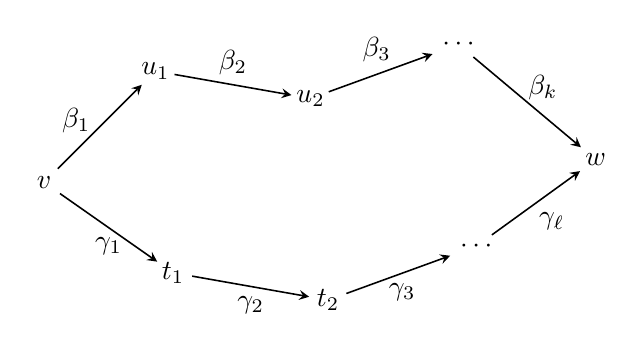
\begin{tikzpicture}[line width = 0.2mm, >=stealth, shorten >= 7pt, shorten <=7pt]
            \draw[->, Black] (0,0) coordinate (a)
            -- node[above, xshift = -0.3cm, yshift = -0.2cm] {$\beta_1$} ++(45:2) coordinate (b);
            \draw[->, Black,] (b)
            -- node[above] {$\beta_2$} ++(-10:2) coordinate (c);
            \draw[->, Black, shorten >= 10pt] (c)
            -- node[above, xshift = -0.1cm] {$\beta_3$} ++(20:2) coordinate (d);
            \draw[->, Black] (d)
            -- node[above, xshift = 0.2cm, yshift = -0.1cm] {$\beta_k$}++(-40:2.275) coordinate (e);
            \node[] at (a) {$v$};
            \node[] at (b) {$u_1$};
            \node[] at (c) {$u_2$};
            \node[] at (d) {$\cdots$}; 
            \node[] at (e) {$w$};
    
            \draw[->, Black] (0,0)
            -- node[below] {$\gamma_1$}++(-35:2) coordinate (f);
            \draw[->, Black] (f)
            -- node[below] {$\gamma_2$}++(-10:2) coordinate (g);
            \draw[->, Black, shorten >= 10pt] (g)
            -- node[below] {$\gamma_3$}++(20:2) coordinate (h);
            \draw[->, Black] (h)
            -- node[below, xshift = 0.2cm] {$\gamma_{\ell}$} (e);
            \node[] at (f) {$t_1$};
            \node[] at (g) {$t_2$};
            \node[] at (h) {$\cdots$};
        \end{tikzpicture}
    \end{center}
    Now consider the image of this diagram in $\mm$, 
    which we do not yet know to be commutative. 
    \begin{center}
        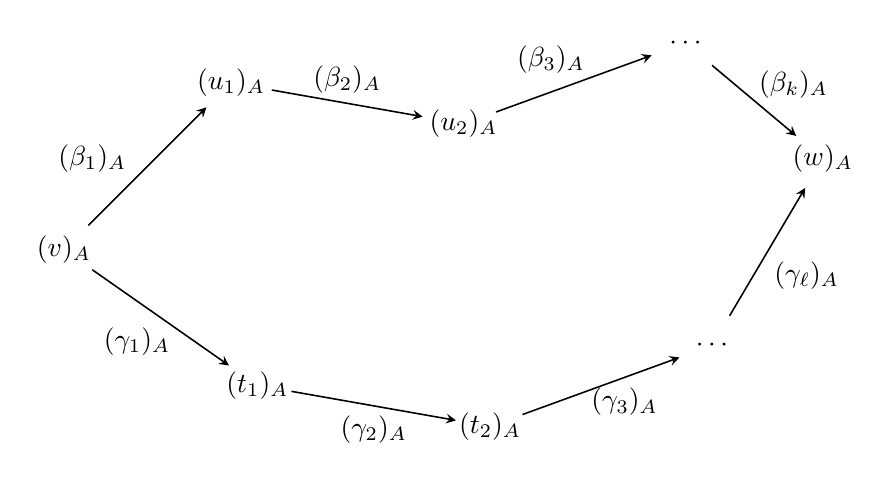
\begin{tikzpicture}[line width = 0.2mm, >=stealth, shorten >= 12.5pt, shorten <=12.5pt]
            \draw[->, Black] (0,0) coordinate (a)
            -- node[above, xshift = -0.7cm, yshift = -0.2cm] {$(\beta_1)_A$}
             ++(45:3) coordinate (b);
            \draw[->, Black,  shorten >= 15pt, shorten <=15pt] (b)
            -- node[above] {$(\beta_2)_A$}
             ++(-10:3) coordinate (c);
            \draw[->, Black, shorten >= 13pt] (c)
            -- node[above, xshift = -0.3cm] {$(\beta_3)_A$}
             ++(20:3) coordinate (d);
            \draw[->, Black] (d)
            -- node[above, xshift = 0.5cm, yshift = -0.1cm] {$(\beta_k)_A$}
            ++(-40:2.275) coordinate (e);
            \node at (a) {$(v)_A$};
            \node at (b) {$(u_1)_A$};
            \node at (c) {$(u_2)_A$};
            \node at (d) {$\cdots$};
            \node at (e) {$(w)_A$};
    
            \draw[->, Black] (0,0)
            -- node[below, xshift = -0.3cm] {$(\gamma_1)_A$}
            ++(-35:3) coordinate (f);
            \draw[->, Black] (f)
            -- node[below] {$(\gamma_2)_A$}
            ++(-10:3) coordinate (g);
            \draw[->, Black, shorten >= 12.5pt] (g)
            -- node[below, xshift = 0.3cm, yshift = 0.1cm] {$(\gamma_3)_A$}
            ++(20:3) coordinate (h);
            \draw[->, Black] (h)
            -- node[below, xshift = 0.5cm] {$(\gamma_{\ell})_A$}
             (e);
            \node at (f) {$(t_1)_A$};
            \node at (g) {$(t_2)_A$};
            \node at (h) {$\cdots$};
        \end{tikzpicture}
    \end{center}
    Our goal is to show that this diagram in $\mm$ is in fact commutative. 
    This will then show our desired equality.
    
    By Proposition \ref{proposition_existence_of_w_to_wn}, we can 
    connect each pure binary word $u_i$ and $t_i$
    to the terminal word $w^{(n)}$ with forward $\alpha$-arrows
    $\Gamma_{u_i}: u_i \to w^{(n)}$ and $\Gamma_{t_i}: t_i \to w^{(n)}$.
    If we add these to our diagram (and suppress the notation on the $\Gamma$'s), 
    it becomes
    \begin{center}
        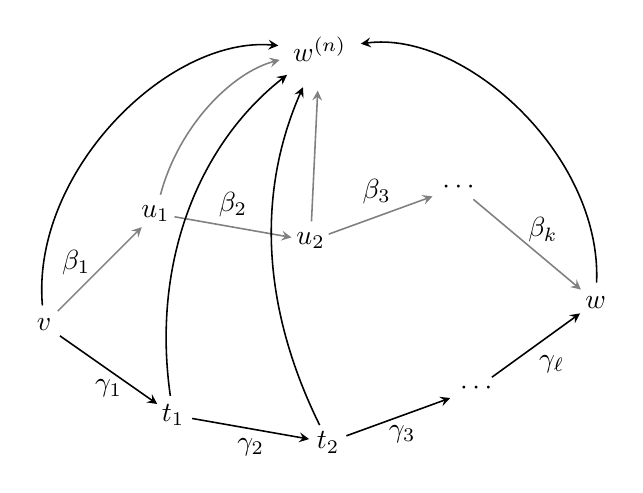
\begin{tikzpicture}[line width = 0.2mm, >=stealth, shorten >= 7pt, shorten <=7pt]
            \draw[->, Black!50!White] (0,0) coordinate (a1)
            -- node[above, xshift = -0.3cm, yshift = -0.2cm] {$\textcolor{Black}{\beta_1}$} ++(45:2) coordinate (a2);
            \draw[->, Black!50!White,] (a2)
            -- node[above] {$\textcolor{Black}{\beta_2}$} ++(-10:2) coordinate (a3);
            \draw[->, Black!50!White, shorten >= 10pt] (a3)
            -- node[above, xshift = -0.1cm] {$\textcolor{Black}{\beta_3}$} ++(20:2) coordinate (a4);
            \draw[->, Black!50!White] (a4)
            -- node[above, xshift = 0.2cm, yshift = -0.1cm] {$\textcolor{Black}{\beta_k}$}++(-40:2.275) coordinate (a5);
            \node at (a1) {$v$};
            \node at (a2) {$u_1$};
            \node at (a3) {$u_2$};
            \node at (a4) {$\cdots$};
            \node at (a5) {$w$};
            
            \draw[->] (0,0)
            -- node[below] {$\gamma_1$}++(-35:2) coordinate (a6);
            \draw[->] (a6)
            -- node[below] {$\gamma_2$}++(-10:2) coordinate (a7);
            \draw[->, shorten >= 10pt] (a7)
            -- node[below] {$\gamma_3$}++(20:2) coordinate (a8);
            \draw[->] (a8)
            -- node[below, xshift = 0.2cm] {$\gamma_{\ell}$} (a5);
            \node at (a6) {$t_1$};
            \node at (a7) {$t_2$};
            \node at (a8) {$\cdots$};
            \coordinate (a9) at (3.5,3.5);
            \node at (a9) {$w^{(n)}$};
            \foreach \n/\ang/\col in {1/50/{Black},2/30/{Black!50!White}, 3/0/{Black!50!White}, 5/-50/{Black}, 6/30/{Black}, 7/25/{Black}}{
                \draw[->, \col, shorten >= 15pt] (a\n) to[bend left = \ang] (a9);
            }
        \end{tikzpicture}
    \end{center}
    whose image under the proxy map in $\mm$ is
    \begin{center}
        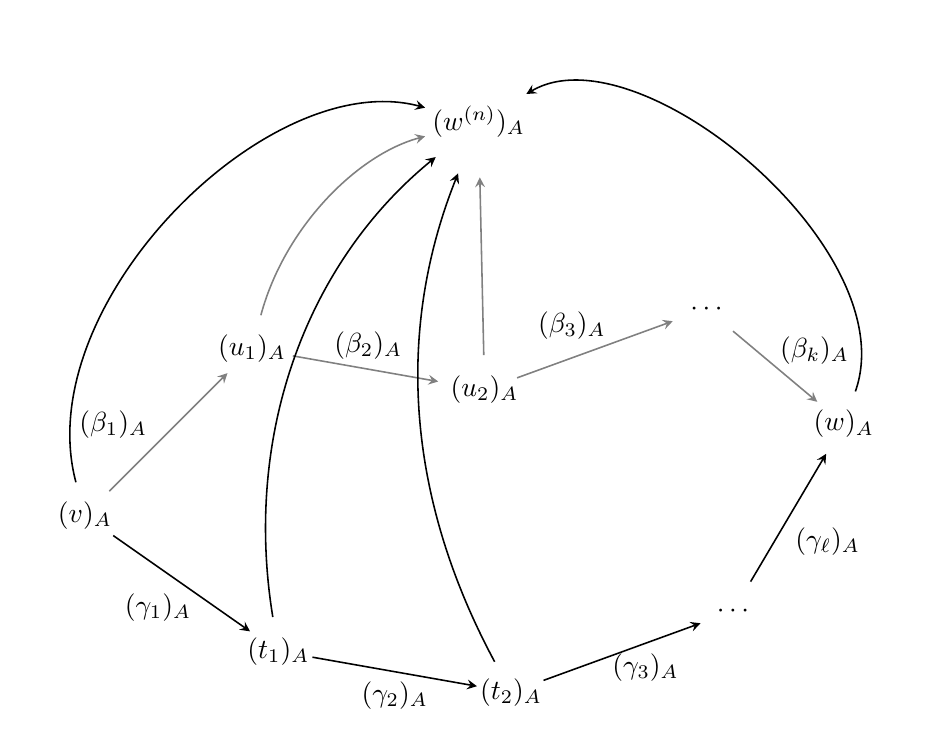
\begin{tikzpicture}[line width = 0.2mm, >=stealth, shorten >= 12.5pt, shorten <=12.5pt]
            \draw[->, Black!50!White] (0,0) coordinate (a1)
            -- node[above, xshift = -0.7cm, yshift = -0.2cm] {$\textcolor{Black}{(\beta_1)_A}$}
             ++(45:3) coordinate (a2);
            \draw[->, shorten >= 17pt, shorten <=15pt, Black!50!White] (a2)
            -- node[above] {$\textcolor{Black}{(\beta_2)_A}$}
             ++(-10:3) coordinate (a3);
            \draw[->, Black!50!White, shorten >= 13pt] (a3)
            -- node[above, xshift = -0.3cm] {$\textcolor{Black}{(\beta_3)_A}$}
             ++(20:3) coordinate (a4);
            \draw[->, Black!50!White] (a4)
            -- node[above, xshift = 0.5cm, yshift = -0.1cm] {$\textcolor{Black}{(\beta_k)_A}$}
            ++(-40:2.275) coordinate (a5);
            \node at (a1) {$(v)_A$};
            \node at (a2) {$(u_1)_A$};
            \node at (a3) {$(u_2)_A$};
            \node at (a4) {$\cdots$};
            \node at (a5) {$(w)_A$};
    
            \draw[->] (0,0)
            -- node[below, xshift = -0.3cm] {$(\gamma_1)_A$}
            ++(-35:3) coordinate (a6);
            \draw[->] (a6)
            -- node[below] {$(\gamma_2)_A$}
            ++(-10:3) coordinate (a7);
            \draw[->, shorten >= 12.5pt] (a7)
            -- node[below, xshift = 0.3cm, yshift = 0.1cm] {$(\gamma_3)_A$}
            ++(20:3) coordinate (a8);
            \draw[->] (a8)
            -- node[below, xshift = 0.5cm] {$(\gamma_{\ell})_A$}
             (a5);
            \node at (a6) {$(t_1)_A$};
            \node at (a7) {$(t_2)_A$};
            \node at (a8) {$\cdots$};
            \coordinate (a9) at (5,5);
            \node at (a9) {$(w^{(n)})_A$};
            \foreach \n/\ang/\col in {1/60/{Black},2/30/{Black!50!White}, 3/0/{Black!50!White}, 5/-70/{Black}, 6/30/{Black}, 7/25/{Black}}{
                \draw[->, \col, shorten >= 20pt] (a\n) to[bend left = \ang] (a9);
            }
        \end{tikzpicture}
    \end{center}
    Thus the diagram has become a cone, with apex $w^{(n)}$, which 
    is sliced by the triangles. The base of this cone is
    the original diagram. We now show that each triangle is commutative.

    Note that each triangle is of two possible forms: it either 
    consists of $\beta_i$ or $\gamma_i$. Without loss of generality, 
    consider a triangle with an instance of $\beta_i$, as below. 
    \begin{center}
        \begin{tikzcd}[column sep = 0.5cm, row sep = 1.4cm]
            (u_{i-1})_A \arrow[dr, swap, "(\Gamma_{u_{i-1}})_A"]
            \arrow[rr, "(\beta_i)_A"]
            &
            &
            (u_i)_A
            \arrow[dl, "(\Gamma_{u_i})_A"]
            \\
            &(w^{(n)})_A&
        \end{tikzcd}
    \end{center}
    Now if $\beta_i$ is a forward $\alpha$-arrow, 
    observe that by Proposition \ref{proposition:parallel_w_to_wn_equal_in_M} 
    it is a commutative diagram in $\mm$. 

    On the other hand, suppose $\beta_i$ is a backward $\alpha$-arrow. 
    Then $\beta_i^{-1}$ is a forward $\alpha$-arrow.
    Then we may rewrite the triangle as 
    \begin{center}
        \begin{tikzcd}[column sep = 0.5cm, row sep = 1.4cm]
            (u_{i-1})_A \arrow[dr, swap, "(\Gamma_{u_{i-1}})_A"]
            \arrow[<-,rr, "(\beta_i^{-1})_A"]
            &
            &
            (u_i)_A
            \arrow[dl, "(\Gamma_{u_i})_A"]
            \\
            &(w^{(n)})_A&
        \end{tikzcd}
    \end{center}
    so that it now consists entirely of forward $\alpha$-arrows. This then 
    allows us to apply Proposition \ref{proposition:parallel_w_to_wn_equal_in_M}  
    to guarantee that it is a commutative diagram in $\mm$. 
    Thus, what we have shown is that  each triangle in the 
    above diagram is commutative in $\mm$. This literally means that 
    for each $i$, 
    \begin{align*}
        (\Gamma_{u_i})_A\circ (\beta_i)_A = (\Gamma_{u_{i-1}})_A
        &\implies 
        (\beta_i)_A = \textcolor{NavyBlue}{(\Gamma_{u_i})_A^{-1} \circ (\Gamma_{u_{i-1}})_A} 
        \\
        (\Gamma_{t_i})_A\circ (\gamma_i)_A = (\Gamma_{t_{i-1}})_A
        &\implies 
        (\gamma_i)_A = \textcolor{Purple}{(\Gamma_{t_i})_A^{-1} \circ (\Gamma_{t_{i-1}})_A}
    \end{align*}
    Therefore, we see that $(\beta_k)_A \circ \cdots \circ (\beta_1)_A$
    can be written as 
    \begin{align*}
        \Big(\textcolor{NavyBlue}{(\Gamma_{u_k})_A^{-1} \circ (\Gamma_{u_{k-1}})_A}\/)
        \circ
        \Big( \textcolor{NavyBlue}{(\Gamma_{u_{k-1}})_A^{-1} \circ (\Gamma_{u_{k-2}})_A}\Big)
        \circ \cdots \circ 
        \Big(\textcolor{NavyBlue}{(\Gamma_{u_1})_A^{-1} \circ (\Gamma_{u_{0}})_A} \Big)
    \end{align*}
    which is a ``telescoping'' composition that reduces to 
    \begin{align*}
        (\Gamma_{u_k})_A^{-1} \circ (\Gamma_{u_{0}})_A.
    \end{align*}
    Similarly, we can expression $(\gamma_{\ell})_A \circ \cdots \circ (\gamma_1)_A$
    as  
    \begin{align*}
        \Big(\textcolor{Purple}{(\Gamma_{t_{\ell}})_A^{-1} \circ (\Gamma_{t_{\ell-1}})_A}\Big)
        \circ 
        \Big(\textcolor{Purple}{(\Gamma_{t_{\ell-1}})_A^{-1} \circ (\Gamma_{t_{\ell-2}})_A}\Big)
        \circ \cdots \circ 
        \Big(\textcolor{Purple}{(\Gamma_{t_1})_A^{-1} \circ (\Gamma_{t_{0}})_A} \Big)
    \end{align*}
    which also reduces to 
    \[
        (\Gamma_{t_{\ell}})_A^{-1} \circ (\Gamma_{t_{0}})_A.
    \]
    However, $u_k = t_{\ell}$ and $u_0 = t_0$, so that 
    \[
        (\Gamma_{u_k})_A^{-1} \circ (\Gamma_{u_{0}})_A
        =
        (\Gamma_{t_{\ell}})_A^{-1} \circ (\Gamma_{t_{0}})_A
        \implies
        (\beta_k)_A \circ \cdots \circ (\beta_1)_A
        =
        (\beta_k)_A \circ \cdots \circ (\beta_1)_A
    \]
    Thus we have that our original diagram in $\mm$
    \begin{center}
        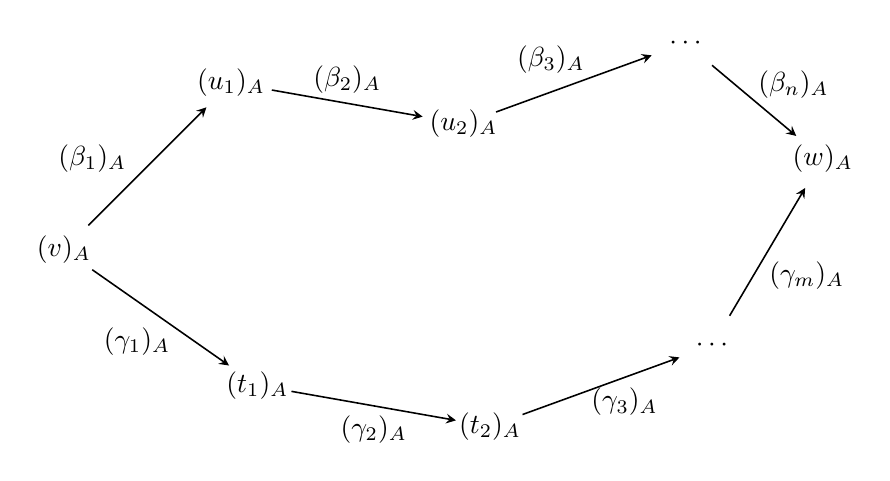
\begin{tikzpicture}[line width = 0.2mm, >=stealth, shorten >= 12.5pt, shorten <=12.5pt]
            \draw[->, Black] (0,0) coordinate (a)
            -- node[above, xshift = -0.7cm, yshift = -0.2cm] {$(\beta_1)_A$}
                ++(45:3) coordinate (b);
            \draw[->, shorten >= 15pt, shorten <=15pt] (b)
            -- node[above] {$(\beta_2)_A$}
                ++(-10:3) coordinate (c);
            \draw[->, shorten >= 13pt] (c)
            -- node[above, xshift = -0.3cm] {$(\beta_3)_A$}
                ++(20:3) coordinate (d);
            \draw[->, Black] (d)
            -- node[above, xshift = 0.5cm, yshift = -0.1cm] {$(\beta_n)_A$}
            ++(-40:2.275) coordinate (e);
            \node at (a) {$(v)_A$};
            \node at (b) {$(u_1)_A$};
            \node at (c) {$(u_2)_A$};
            \node at (d) {$\cdots$};
            \node at (e) {$(w)_A$};
    
            \draw[->, Black] (0,0)
            -- node[below, xshift = -0.3cm] {$(\gamma_1)_A$}
            ++(-35:3) coordinate (f);
            \draw[->, Black] (f)
            -- node[below] {$(\gamma_2)_A$}
            ++(-10:3) coordinate (g);
            \draw[->, Black, shorten >= 12.5pt] (g)
            -- node[below, xshift = 0.3cm, yshift = 0.1cm] {$(\gamma_3)_A$}
            ++(20:3) coordinate (h);
            \draw[->, Black] (h)
            -- node[below, xshift = 0.5cm] {$(\gamma_m)_A$}
                (e);
            \node at (f) {$(t_1)_A$};
            \node at (g) {$(t_2)_A$};
            \node at (h) {$\cdots$};
        \end{tikzpicture}
    \end{center}
    is commutative. Therefore we have that 
    parallel sequences of $\alpha$-arrows are equal in $\mm$, as desired.
\end{prf}

Finally, we use all of our previous work to prove Theorem \ref{theorem:coherence_in_alpha}.
In this case, the proof is simply the definition of our desired functor.
We state the theorem here for the reader's convenience.

\begin{customthm}{\ref{theorem:coherence_in_alpha}}[Associator Coherence.]
    Let $(\mm, \otimes, I, \alpha, \lambda, \rho)$ be a monoidal category. 
    For every object $A$, there exists a unique functor 
    $\Phi_A: \ww_P \to \mm$ which agrees with the proxy map $(-)_A$ on the objects and $\alpha$-arrows.
\end{customthm}

To define this functor, we will (in this order) define the functor on 
(1) object, (2) $\alpha$-arrows, (3) general morphisms of $\wp$, and then 
finally show that our definition preserves composition.

\begin{description}
    \item[Objects.] 
    For a pure binary word $w$, we define $\Phi_A(w) = (w)_A$.

    \item[Morphisms.] 
    \begin{itemize}
        \item[(1)] If $\beta$ is an $\alpha$-arrow, we define 
        $\Phi_A(\beta) = (\beta)_A$. 
        
        \item[(2)] 
        Now we define our functor on a general morphism $v \to w$ in $\wp$. For convenience 
        denote this as $\phi_{v,w}: v \to w$. 
        
        We know by 
        Corollary \ref{corollary:morphisms_of_wp} that there exist finitely many 
        forward and backward $\alpha$-arrows $\gamma_1, \dots, \gamma_k$ such  that 
        \[
            \phi_{v,w} = \gamma_k \circ \cdots \circ \gamma_1. 
        \]
        Therefore, define 
        \[
            \Phi_A(\phi_{v,w}) = \Phi(\gamma_k \circ \cdots \circ \gamma_1)= (\gamma_k)_A \circ \cdots \circ (\gamma_1)_A.
        \]
        By Proposition \ref{proposition:parallel_in_M_are_equal}, we see that 
        this definition is well-defined.  
    \end{itemize}
    Note that this definition allows the functor to also be well-defined 
    on identities, i.e., in all instances, $\Phi_A(1_u) = 1_{u_A}$.

    We now show that this definition of our functor behaves under composition.
    Let $\phi_{u,v}: u \to v$ and $\phi_{v,w}: v \to w$ be morphisms in 
    $\wp$. Then there exist sequences of $\alpha$-arrows 
    $\beta_1, \dots, \beta_k$ and $\gamma_1, \dots, \gamma_{\ell}$ 
    such that 
    \begin{gather*}
        \phi_{u,v}= \beta_k \circ \cdots \circ \beta_1 \qquad
        \phi_{v,w} = \gamma_{\ell} \circ \cdots \circ \gamma_1.
    \end{gather*}
    Then we can write 
    \begin{align*}
        \Phi(\phi_{v,w} \circ \phi_{u,v}) &= \Phi(\gamma_{\ell} \circ \cdots \circ \gamma_1 \circ \beta_k \circ \cdots \circ \beta_1)\\
        &= (\gamma_{\ell})_A \circ \cdots \circ (\gamma_1)_A \circ (\beta_k)_A \circ \cdots \circ (\beta_1)_A\\
        &= \Phi(\gamma_{\ell} \circ \cdots \circ \gamma_1) \circ \Phi(\beta_k \circ \cdots \circ \beta_1)\\
        &= \Phi(\phi_{v,w}) \circ \Phi(\phi_{u,v})
    \end{align*}
    Hence we see that our definition on morphisms behaves appropriately on composition, 
    so that $\Phi$ is in fact a functor. 
\end{description}

    We conclude this section by proving the Diamond Lemma, which we have now 
    seen to play a critical role in this proof. 
    \begin{customlemma}{\ref{lemma:diamond_lemma}}[Diamond Lemma]
        Let $w$ be a pure binary word and suppose $\beta_1,\beta_2$ are two 
        forward $\alpha$-arrows as below.
        \begin{center}
            \begin{tikzcd}[column sep = 1.4cm, row sep = 1cm]
                &
                w
                \arrow[dl, swap, "\beta_1"]
                \arrow[dr, "\beta_2"]
                &
                \\
                w_1
                &
                &
                w_2
            \end{tikzcd}
        \end{center}
        There exists a pure binary word $z$ and two $\gamma_1: w_1 \to z, \gamma_2: w_2 \to z$,
        with $\gamma_1, \gamma_2$ a composition of forward $\alpha$-arrows,
        such that for any monoidal category 
        $(\mm, \otimes, I, \alpha, \lambda, \rho)$ the diagram below is 
        commutative in $\mm$.
        \begin{center}
            \begin{tikzcd}[column sep = 1.4cm, row sep = 1cm]
                &
                (w)_A
                \arrow[dl,swap, "(\beta_1)_A"]
                \arrow[dr, "(\beta_2)_A"]
                &
                \\
                (w_1)_A
                \arrow[dr, Green, swap,"(\gamma_1)_A"]
                && 
                (w_2)_A
                \arrow[dl, Green, "(\gamma_2)_A"]
                \\
                &(z)_A&
            \end{tikzcd}
        \end{center}
        is commutative. 
    \end{customlemma}

    As we said before, the above lemma is an existence result, 
    so we emphasize this fact by coloring 
    the arrows, which we are asserting to exist, Green. 

    \begin{prf}
        We will prove this using induction on the length of $w = u \otimes v$.
        Therefore, throughout the proof, suppose the result is already true for all words of length less than that 
        of $w$. 

        We proceed in a case-by-case basis, exhausting the possible forms of $\beta_1$ and $\beta_2$.
        For our purposes, we will express $w = u \otimes v$. 
        Whenever $\ll(v) > 1$, we write $v= s \otimes t$. 
        
        Let $\beta_1, \beta_2$ be forward $\alpha$-arrows. 
        Then $\beta_1$ could be of the forms
        \[
            \alpha_{u,s,t}\qquad 1_u \otimes \gamma_1 \qquad \gamma_1\otimes 1_v
        \]
        and $\beta_2$ could be of the forms 
        \[
            \alpha_{u,s,t}\qquad 1_u\otimes\gamma_2 \qquad \gamma_2\otimes 1_v.
        \]
        with $\gamma_1, \gamma_2$ already forward $\alpha$-arrows.
        Therefore, our cases for $\beta_1,\beta_2$, 
        displayed in tuples, are listed in the table below.
        \begin{center}
            \begin{tabular}{ p{1.2cm} |p{3cm} p{3cm} p{3cm}  }
                $(\beta_1,\beta_2)$
                &
                $\alpha_{u,s,t}$
                &
                $1_u\otimes \gamma_2$
                &
                $\gamma_2 \otimes 1_v$
                \\[0.2cm]
                \hline
                $\alpha_{u,s,t}$
                &
                $\textcolor{Red}{(\alpha_{u,s,t}, \alpha_{u,s,t})}$ & $\textcolor{NavyBlue}{(\alpha_{u,s,t},1_u \otimes \gamma_2)}$ 
                & $\textcolor{Orange}{(\alpha_{u,s,t}, \gamma_2\otimes 1_v)}$\\[0.2cm]
                $1_u \otimes \gamma_1$
                &
                $\textcolor{NavyBlue}{(1_u \otimes \gamma_1, \alpha_{u,s,t})}$ 
                & $\textcolor{Magenta}{(1_u \otimes \gamma_1 ,1_u \otimes \gamma_2)}$ 
                & $\textcolor{Purple}{(1_u \otimes \gamma_1, \gamma_2\otimes 1_v)}$\\[0.2cm]
                $\gamma_1\otimes 1_v$
                &
                $\textcolor{Orange}{(\gamma_1\otimes 1_v, \alpha_{u,s,t})}$ 
                & $\textcolor{Purple}{(\gamma_1\otimes 1_v ,1_u \otimes \gamma_2)}$ 
                & $\textcolor{ProcessBlue}{(\gamma_1\otimes 1_v, \gamma_2\otimes 1_v)}$\\[0.2cm]
                \end{tabular}
        \end{center}    
        While there are 9 cases displayed above, we have pointed out via color the pairs of cases which are logically 
        equivalent to each other due to the symmetry of our problem. Therefore, we actually have 6 cases to check 
        We now proceed to the proof.
    
        \noindent\textbf{Case 1:} $\textcolor{Red}{(\alpha_{u,s,t}, \alpha_{u,s,t})}.$\\
        In this case, we have that $\beta_1 =  \beta_2$, for which the statement is trivially true.
        \\

        \noindent\textbf{Case 2:} $\textcolor{Purple}{(\gamma_1\otimes 1_v ,1_u \otimes \gamma_2)}$\\
        Suppose $\beta_1 = \gamma_1 \otimes 1_v$ and $\beta_2 = 1_u\otimes \gamma_2$. 
        Here, $\gamma_1: u \to u'$ and $\gamma_2: v \to  v'$ for some pure binary 
        words $ u',v'$. Then we get the diagram 
        \begin{center}
            \begin{tikzcd}[column sep = 1.4cm, row sep = 1cm]
                &
                u \otimes v
                \arrow[dr, "1_u \otimes \gamma_2 "]
                \arrow[dl, swap, "\gamma_1 \otimes 1_v"]
                &
                \\
                u'\otimes v
                \arrow[dr, Green, swap, "1_{u'}\otimes \gamma_2"]
                &
                &
                u\otimes v'
                \arrow[dl, Green, "\gamma_1 \otimes 1_{v'}"]
                \\
                &
                u'\otimes v'
                &
            \end{tikzcd}
        \end{center}
        which commutes by the bifunctoriality of $\otimes$. 
        \\
        \\
        \textbf{Case 3:} $\textcolor{ProcessBlue}{(\gamma_1\otimes 1_v, \gamma_2\otimes 1_v)}$\\
        Suppose $\beta_1 = \gamma_1 \otimes 1_v$ and $\beta_2 = \gamma_2 \otimes 1_v$
        with $\gamma_1: u \to u_1$ and $\gamma_2: u \to u_2$ both forward $\alpha$-arrows.
        % We prove this case by induction on the length. 
        % Suppose the result is true in this case, for all binary words of length less than $k$.
        % Let $w = u \otimes v$ have length $k+1$. 
        Then in this case we have the triangle below in $\mm$.
        \begin{center}
            \begin{tikzcd}[column sep = 1cm, row sep = 1cm]
                &
                (u \otimes v)_A
                \arrow[dr, "(\gamma_2)_A \otimes 1_{(v)_A}"]
                \arrow[dl, swap, "(\gamma_1)_A\otimes 1_{(v)_A}"]
                &
                \\
                (u_1 \otimes v)_A
                &
                &
                (u_2\otimes v)_A
            \end{tikzcd}
        \end{center}
        Note that the above diagram 
        is the image of diagram 
        \begin{center}
            \begin{tikzcd}[column sep = 1.4cm, row sep = 1cm]
                &
                (u)_A
                \arrow[dr, "(\gamma_2)_A "]
                \arrow[dl, swap, "(\gamma_1)_A"]
                &
                \\
                (u_1)_A
                &
                &
                (u_2)_A
            \end{tikzcd}
        \end{center}
        under the functor $(-)\otimes (v)_A$. As $\ll(u) < \ll(u\otimes v)$, 
        we know by our induction hypothesis that 
        there exists a pure binary word $z$
        and a pair of composite, forward $\alpha$-arrows $\sigma_1: u_1 \to z$ and 
        $\sigma_2: u_2 \to z$ such that the diagram below commutes in $\mm$.
        \begin{center}
            \begin{tikzcd}[column sep = 1.4cm, row sep = 1cm]
                &
                (u)_A
                \arrow[dr, "(\gamma_2)_A"]
                \arrow[dl, swap, "(\gamma_1)_A"]
                &
                \\
                (u_1)_A
                \arrow[dr, swap, "(\sigma_1)_A"]
                &
                &
                (u_2)_A
                \arrow[dl, "(\sigma_2)_A"]
                \\
                &
                (z)_A
                &
            \end{tikzcd}
        \end{center}
        Therefore we can apply the functor 
        $(-)\otimes (v)_A$ on the above diagram 
        to obtain the commutative diagram below
        \begin{center}
            \begin{tikzcd}[column sep = 0.8cm, row sep = 1cm]
                &
                (u)_A \otimes (v )_A
                \arrow[dr, "(\gamma_1)_A \otimes (1_v)_A"]
                \arrow[dl, swap, "(\beta_2)_A \otimes (1_v)_A"]
                &
                \\
                (u_1)_A \otimes (v)_A
                \arrow[dr, Green, swap, "(\sigma_1)_A \otimes (1_v)_A"]
                &
                &
                (u_2)_A \otimes  (v)_A
                \arrow[dl, Green, "(\sigma_2) \otimes  (1_v)_A"]
                \\
                &
                (z)_A \otimes (v)_A
                &
            \end{tikzcd}
        \end{center}
        which proves this case.
        \\
        \\
        \textbf{Case 4:} $\textcolor{Magenta}{(1_u \otimes \gamma_1 ,1_u \otimes \gamma_2)}$\\
        The next case is when $\beta_1 = 1_u \otimes \gamma_1$ and $\beta_2 = 1_u\otimes\gamma_2$  
        with $\gamma_1: v \to v_1$ and $\gamma_2: v \to v_2$. However, this can be proved 
        in a similar manner as the previous case using 
        the induction hypothesis and the functor $(u)_A \otimes (-)$.
        \\
        \noindent\textbf{Case 5:} $\textcolor{Orange}{(\alpha_{u,s,t}, \gamma_2\otimes 1_v)}$\\
        Let $\beta_1 = \alpha_{u,s,t}$,  so that $w = u \otimes (s \otimes t)$. 
        Let $\beta_2 = \gamma_2 \otimes 1_{v}
        = \gamma_2 \otimes 1_{s\otimes t}$ 
        with $\gamma_2: u \to u'$
        a forward $\alpha$-arrow. Then we will have the diagram in $\mm$
        \begin{center}
            \begin{tikzcd}[column sep = 0.8cm, row sep = 1cm]
                &
                (u \otimes (s\otimes t))_A
                \arrow[dr, "(\gamma_2\otimes (1_s \otimes 1_t))_A"]
                \arrow[dl, swap, "(\alpha_{u,s,t})_A"]
                &
                \\
                ((u\otimes s)\otimes t)_A
                \arrow[dr,Green,  swap, "((\gamma_2 \otimes 1_s)\otimes 1_t)_A"]
                &
                &
                (u'\otimes(s\otimes t))_A
                \arrow[dl, Green, "(\alpha_{u', s,t})_A"]
                \\
                &
                ((u'\otimes s)\otimes t)_A
                &
            \end{tikzcd}
        \end{center}
        which commutes in $\mm$ by naturality of $\alpha$. 
        \\
        \\
        \textbf{Case 6:} $\textcolor{NavyBlue}{(\alpha_{u,s,t},1_u \otimes \gamma_2)}$\\
        Let $\beta_1 = \alpha_{u,s,t}$, $\beta_2 = 1_u \otimes \gamma$
        with $\gamma$ a forward $\alpha$-arrow with domain $s \otimes t$. 
        By the recursive definition of a forward $\alpha$-arrow, 
        we have three possible cases for $\gamma$.
        \\
        \\
        \textbf{Case 6.1: }$\gamma = 1_s \otimes \gamma'$\\
        With $\gamma = 1_s \otimes \gamma'$ with $\gamma' : t\to t'$ 
        already a forward $\alpha$-arrow,
        we have the diagram in $\mm$
        \begin{center}
            \begin{tikzcd}[column sep = 1.4cm, row sep = 1cm]
                &
                (u \otimes (s\otimes t))_A
                \arrow[dr, "(1_u\otimes(1_s \otimes \gamma))_A"]
                \arrow[dl, swap, "(\alpha_{u,s,t})_A"]
                &
                \\
                ((u\otimes s)\otimes t)_A
                \arrow[dr,Green,  swap, "((1_u\otimes 1_s)\otimes \gamma)_A"]
                &
                &
                (u\otimes(s\otimes t'))_A
                \arrow[dl,Green, "(\alpha_{u,s,t'})_A"]
                \\
                &
                ((u\otimes s)\otimes t')_A
                &
            \end{tikzcd}
        \end{center}
        which commutes in $\mm$ by naturality of $\alpha$.
        \\
        \\
        \textbf{Case 6.2:} $\gamma = \gamma' \otimes 1_t$\\
        If $\gamma = \gamma' \otimes 1_t$ with $\gamma': s \to s'$ 
        already a forward $\alpha$-arrow, we can create the diagram 
        \begin{center}
            \begin{tikzcd}[column sep = 1.4cm, row sep = 1cm]
                &
                (u \otimes (s\otimes t))_A
                \arrow[dr, "(1_u\otimes(\gamma' \otimes 1_t))_A"]
                \arrow[dl, swap, "(\alpha_{u,s,t})_A"]
                &
                \\
                ((u\otimes s)\otimes t)_A
                \arrow[dr, Green, swap, "((1_u\otimes \gamma')\otimes 1_t)_A"]
                &
                &
                (u\otimes(s' \otimes t))_A
                \arrow[dl, Green, "(\alpha_{u,s',t})_A"]
                \\
                &
                ((u\otimes s')\otimes t)_A
                &
            \end{tikzcd}
        \end{center}
        which also commutes in $\mm$ by naturality of $\alpha$.
        \\
        \textbf{Case 6.3:} $\gamma = \alpha_{s,p,q}$\\
        The third case for $\gamma$ is when $\gamma = \alpha_{s,p,q}$. 
        In this case, we 
        express $w = u\otimes (s\otimes (p \otimes q))$. 
        We can then construct the diagram  
        \begin{center}
            \begin{tikzcd}[column sep = 1.4cm, row sep = 1.5cm]
                &
                (u\otimes(s\otimes(p\otimes q)))_A
                \arrow[dl, swap, "(\alpha_{u, s, p\otimes q})_A"]
                \arrow[dr, "(1_u\otimes\alpha_{s,p,q})_A"]
                &
                \\
                ((u\otimes s)\otimes(p\otimes q))_A
                \arrow[d, Green, swap, "(\alpha_{u\otimes s, p ,q})_A"]
                &
                &
                (u\otimes((s\otimes p)\otimes q))_A
                \arrow[d, "(\alpha_{u, s\otimes p, q})_A"]
                \\
                (((u\otimes s)\otimes p)\otimes q)_A
                &
                &
                ((u\otimes(s\otimes p))\otimes q)_A
                \arrow[ll, Green, "(\alpha_{u,s,p}\otimes 1_q)_A"]
            \end{tikzcd}
        \end{center}
        which is always commutative in $\mm$.
        In this case, the word $((u\otimes s)\otimes p)\otimes q$
        acts as our vertex $z$ which completes the diagram. 

        As we have exhausted all possible cases,
        we see that the statement is true for pure binary words of rank $k+1$
        if it is true for all pure binary words with rank at most $k$.
        By induction, the statement is true for all binary words of any rank, 
        so that we have proved the theorem.
    \end{prf}

\newpage
\subsection*{Step Four: Binary Words}

So far we have established a unique functor $\Phi_A: \wp \to \mm$ 
for each object $A$ of any given monoidal category $\mm$,
and this functor grants us coherence in the associators between iterated 
monoidal products of a single object.
We now consider such monoidal products with the identity $I$ as well, 
so that we may say something about coherence with regard to the 
unitors $\lambda$ and $\rho$ in a general monoidal category. 
Towards that goal, we now consider binary words (not just pure binary words)
and introduce some definitions.

Recall that $\ll$ calculates the length of a binary word, or more informally, 
the number of $x_1$'s in a binary word. We now introduce a dual quantity which 
instead counts the number of $x_0$

\begin{definition}
    Let $w$ be a binary word. Define the \textbf{identity length} of $w$, 
    denoted $\mathcal{E}$, recursively as follows. 
    \begin{itemize}
        \item $\ee(x_0) = 1$ and $\ee(x_1) = 0$.
        \item $\ee(u \otimes v) = \ee(u) + \ee(v)$.
    \end{itemize}
\end{definition}

Similarly to how $\ll(-)$ counts the number of $x_1$'s in a binary word, $\ee(-)$ 
counts the number of $x_0$'s in a binary word.

Next, we introduce the following concept that will later on 
be key to our proof of Mac Lane's Coherence Theorem.
\begin{definition}
    Let $w$ be a binary word. 
    We define the \textbf{clean word} derived from $w$,
    denoted $\overline{w}$, recursively as follows. 
    \begin{itemize}
        \item We set $\overline{x_1} = x_1$. 
        \item If $\ll(w) = 0$ (i.e., it has no instance of $x_1$) then $\overline{w} = x_0$. 
        \item Let $u,v$ be binary words with $\ll(u) = 0$ and $\ll(v) > 0$. 
        Then
        \[
            \overline{u \otimes v} = \overline{v \otimes u} = \overline{v}
        \]
        \item Let $u,v$ be binary words with $\ll(u), \ll(v) > 0$. Then 
        $\overline{u\otimes v} =  \overline{u} \otimes \overline{v}$. 
    \end{itemize}
\end{definition}

Note that for a pure binary word $w$, we have that $\overline{w} =w$.
Informally, the clean word of a binary word of nonzero length is simply the pure 
binary word obtained by removing all instances of the identity from its 
expression. In the case for a binary word with zero length, we naturally define 
the clean word to be $x_0$ .

\begin{example}
    We offer some examples of clean words obtained from binary words.
    \begin{center}
        \begin{tabular}{|c | c|}
            \hline
            Word & Clean Word\\
            \hline
            $x_0\otimes (x_0 \otimes x_0)$ & $x_0$\\
            $x_0 \otimes (x_1 \otimes x_0)$ & $x_1$\\
            $(x_1 \otimes x_0) \otimes x_1$ & $x_1 \otimes x_1$ \\
            $((x_1 \otimes x_0) \otimes x_0)\otimes x_1$ & $x_1 \otimes x_1$\\
            $(x_1 \otimes x_0) \otimes ((x_1 \otimes x_0) \otimes x_1)$ & $x_1 \otimes (x_1 \otimes x_1)$\\
            \hline
        \end{tabular}
    \end{center}
    The above example also shows that two different binary words 
    can have the same clean word. 
\end{example}


\begin{definition}[Monoidal Arrows]
    A \textbf{forward monoidal} arrow of $\ww$ is defined recursively as follows. 
    \begin{itemize}
        \item For any triple of binary words $u, v, w$, the morphisms 
        \begin{align*}
            \alpha_{u, v, w}&: u \otimes (v \otimes w) \isomarrow (u \otimes v)\otimes w\\
            \lambda_{u}&: x_0 \otimes u \isomarrow u\\
            \rho_{u}&: u\otimes x_0 \isomarrow u
        \end{align*}
        are, respectively, \textbf{forward} $\alpha$-, $\lambda$-, and $\rho$-\textbf{arrows}. 
        They are collectively 
        defined to be \textbf{forward monoidal arrows}. 
        \item For any binary word $u$ and forward monoidal arrow $\mu$, the morphisms
        \[
            1_{u} \otimes \mu \qquad \mu \otimes 1_{u}
        \]
        are forward monoidal arrows.
    \end{itemize}
    Finally, we say a \textbf{backward monoidal arrow} 
    is the inverse of a forward monoidal arrow. 
\end{definition}

We also establish the following terminology to distinguish our $\alpha$-arrows 
from our $\lambda$ and $\rho$ arrows.

\begin{definition}
    A \textbf{forward unitor arrow} is either a forward $\lambda$-arrow or a forward $\rho$-arrow.
    Similarly, a  \textbf{backward unitor arrow} is the inverse of a forward unitor arrow.
\end{definition}
 
As we have already seen forward $\alpha$-arrows, 
we provide examples of forward and backward $\lambda, \rho$-arrows.

\begin{example}
    Below we have a forward and backward $\lambda$-arrow.
    \begin{center}
        \begin{tikzcd}
            x_1 \otimes ((x_0 \otimes x_1)\otimes x_1)
            \arrow[d, "1_{x_1}\otimes(\lambda_{x_1}\otimes 1_{x_1})"]
            \\
            x_1 \otimes (x_1 \otimes x_1)
        \end{tikzcd}
        \hspace{1cm}
        \begin{tikzcd}
            (x_1\otimes x_1)\otimes x_1
            \arrow[d, "\lambda^{-1}_{(x_1\otimes x_1)\otimes x_1}"]
            \\
            x_0\otimes ((x_1 \otimes x_1)\otimes x_1)
        \end{tikzcd}
    \end{center}
    We also have forward and backward $\rho$-arrows below.
    \begin{center}
        \begin{tikzcd}
            (x_1\otimes x_0)\otimes x_1
            \arrow[d, "\rho_{x_1}\otimes 1_{x_1}"]
            \\
            x_1 \otimes x_1
        \end{tikzcd}
        \hspace{1cm}
        \begin{tikzcd}
            x_1\otimes(x_1\otimes x_1)
            \arrow[d, "1_{x_1}\otimes \rho^{-1}_{x_1\otimes x_1}"]
            \\
            x_1\otimes((x_1\otimes x_1)\otimes x_0)
        \end{tikzcd}
    \end{center}
\end{example}

We now move onto proving some important lemmas regarding 
monoidal arrows that we will use for the coherence theorem.

The first three are quick, but have particular importance. 
\begin{lemma}\label{lemma:ee(w)=0_iff_w_is_clean}
    Let $w$ be a binary word, $w \ne x_0$. 
    Then $\ee(w) = 0$ if and only if $w = \overline{w}$. 
\end{lemma}

Note that $w = x_0$ is the only case for which the above proposition is not true, 
since $x_0 = \overline{x_0}$ but $\ee(x_0) \ne 0$. Hence,
our reasoning for excluding it (and it is not a case we will need to concern ourselves with).

\begin{prf}
    Suppose $\ee(w) = 0$, and let us prove the forward direction by induction on 
    the length of the word. 
    Let us write $w = u \otimes v$, suppose that the statement is true for all pure binary words with 
    length less than $w$. Observe that  
    \[
        w = u \otimes v = \overline{u} \otimes \overline{v} = \overline{u \otimes v} = \overline{w}.
    \]
    where we used the induction hypothesis on $u, v$ which have smaller length than 
    $w$. Thus we see that $w = \overline{w}$. 

    Conversely, suppose $\overline{w} = w$, $w \ne x_0$, and suppose the statement is true for binary words 
    with length less than $w$. Write $w  = u \otimes v$. 
    By the definition 
    of a clean word, the only way we can have $\overline{w} = w$ is if $u,v$ 
    are binary words with nonzero length. 
    Therefore, if $\overline{w} = w$ we see that 
    \[
        \overline{u} \otimes \overline{v} = u \otimes v.
    \]
    Since $u, v$ have smaller length than $w$, we may use the induction 
    hypothesis to conclude that $\ee(u) = \ee(v) = 0$. Hence, 
    $\ee(w) = 0$, as desired. 
\end{prf}

\begin{lemma}\label{lemma:unitors_decrease_unit_length}
    Let $w$ be a binary word. Suppose
    $\iota: w \to w'$ is a forward unitor arrow. 
    Then $\ee(w') = \ee(w) - 1$. 
\end{lemma}

In other words, any unitor arrow always takes away exactly one identity.

\begin{prf}
    We prove this by examining the possible cases for $\iota$. 
    Write $w = u \otimes v$.
    As $\iota$ is a forward unitor arrow, it has four possible forms. 

    \begin{itemize}
        \item[(1)] Suppose $\iota = \lambda_v: x_0 \otimes v \to v$. 
        As 
        \[
            \ee(v) = \ee(v) + \ee(x_0) - 1 = \ee(v \otimes x_0) - 1   
        \]
        we see that the statement is satisfied in this case.

        \item[(2)] If $\iota = \rho_u: u \otimes x_0 \to u$,
        we can use a similar argument as in (1) to prove the statement.

        \item[(3)] Suppose $\iota = 1_{u} \otimes \kappa: u \otimes v \to u \otimes v'$ 
        where $\kappa: v \to v'$ is a forward unitor arrow for which the 
        statement is already true. Then $\ee(v') = \ee(v) - 1$. Hence, 
        \[
            \ee(u \otimes v') = \ee(u \otimes v) - 1. 
        \]
        Therefore the statement is satisfied for $1_u \otimes \kappa$ if it is 
        true for $\kappa$. 

        \item[(4)] If $\iota = \kappa \otimes 1_v: u \otimes v \to u' \otimes v$
        where $\kappa$ is a forward unitor for which the statement is already true, 
        then we may prove this case by following a similar argument as in (3). 
    \end{itemize}
    As we have examined all cases, we may conclude that for every 
    forward unitor $\iota: w \to w'$, we have that $\ee(w') = \ee(w) - 1$ 
    as desired. 
\end{prf}

\begin{lemma}\label{lemma:unitors_preserve_clean_word}
    Let $\iota: w \to w'$ be a forward unitor arrow. Then 
    $\overline{w} = \overline{w}'$. 
\end{lemma}

In other words, unitor arrows do not alter the particular format of a
clean word.

\begin{prf}
    First, observe that the result is trivial if $\ll(w) = \ll(w') = 0$. 
    Therefore, let $w = u \otimes v$ be such a binary 
    word with $\ee(w) > 0$.
    Suppose the statement is true for 
    binary words $v$ such that $\ee(v) < \ee(w)$. 
    Let $\iota:w \to w'$ be a forward unitor arrow. 
    By the recursive definition of $\iota$, our forward unitor arrow has 
    four possible forms. 

    \begin{itemize}
        \item[(1)] Suppose $\iota = \lambda_v: x_0 \otimes v \to v$. 
        However, note that $\overline{x_0 \otimes v} = \overline{v}$, 
        so that this case is true. 
        
        \item[(2)] If $\iota = \rho_u: u \otimes x_0 \to u$, 
        then this case may be proven in a similar manner as case (1).

        \item[(3)] Suppose 
        $\iota = 1_u \otimes \kappa: u \otimes v \to u \otimes v'$ where 
        $\kappa$ is a forward unitor arrow for which the result is already true. 
        Since $\ll(u \otimes v) < 0$, we have a few subcases. 

        Suppose $\ll(v) > 0$. 
        Then by our assumption on $\kappa$, 
        $\overline{v} = \overline{v}'$.
        Therefore, if 
        $\ll(u) = 0$, we see that 
        \[
            \overline{u \otimes v} = \overline{v} 
            = \overline{v}' = \overline{u \otimes v}'
        \]
        which satisfies this case. 
        If instead $\ll(u) > 0$, then 
        \[
            \overline{u \otimes v} = \overline{u}\otimes\overline{v} = 
            \overline{u}\otimes\overline{v}' = \overline{u \otimes v}'
        \]
        which again satisfies the case. 

        Finally, suppose $\ll(v) = 0$. 
        Then $\overline{u \otimes v} = 
        \overline{u} = \overline{u \otimes v}'$. 

        In all cases we see that $\overline{u \otimes v} = \overline{u \otimes v}'$ 
        as desired. 

        \item[(3)] Our third case if when $\iota = \kappa \otimes 1_v: u \otimes v \to u' \otimes v$ 
        with $\kappa$ a forward  unitor for which the result is already true. However, this 
        case can be proved similarly as in case (2).
    \end{itemize}
    In all instances, we see that for a forward unitor arrow $\iota: w \to w'$, 
    we have that $\overline{w} = \overline{w}'$, as desired. 
\end{prf}

The following lemma is an important existence result that will be used in the 
next proposition.

\begin{lemma}\label{lemma:existence_w_to_clean_w}
    Let $w$ be a binary word with $\ee(w) > 0$.
    Then there exists a forward unitor with domain $w$.
\end{lemma}

\begin{prf}
    We prove this by induction on the total length of a binary word 
    $\ll(w) + \ee(w)$. 
    Thus, let $w = u \otimes v$ be a binary word with $\ee(w) > 0$ 
    and suppose the statement is true 
    for all binary words $z$ with
    \[
        \ll(z) + \ee(z) < \ll(w) + \ee(w).
    \]
    Then we have a few cases for $w$. 
    \begin{itemize}
        \item[(1)] Suppose $u = x_0$. Then we take the forward unitor 
        $\lambda_v: x_0 \otimes v \to v$.

        \item[(2)] Suppose $v = x_0$. We may similarly take $\rho_u: u \otimes x_0 \to u$, 
        so that this case is satisfied. 
        
        \item[(3)] Suppose $u, v \ne x_0$. Since $\ee(w) > 1$, 
        either $\ee(u)$ or $\ee(v) > 0$. Without loss of generality, suppose 
        $\ee(u) > 0$. Since 
        \[
            \ll(u) + \ee(u) = \ll(u) + \ee(u)
        \]
        we may apply our induction hypothesis to conclude that there exists 
        a forward unitor $\iota: u \to u'$ with domain $u$. 
        Hence, the morphism 
        \[
            \iota \otimes 1_v : u \otimes v \to u' \otimes v
        \]
        is a forward unitor with domain $u \otimes v = w$. 
    \end{itemize}
    As we have evaluated all cases, we see that the statement is true for all
    binary words as desired. 
\end{prf}

The previous four lemmas now give rise to the following proposition. 
\begin{proposition}\label{proposition:exists_w_to_clean_w}
    Let $w$ be a binary word with $\ee(w) = \ell$. Then there exists a 
    composable sequence of
    ${\ell}$-many forward unitor arrows $\iota_{\ell}, \cdots, \iota_1$ as below:
    \[
        \iota_{\ell} \circ \cdots \circ \iota_1: w \to w'.
    \]
    Moreover, for every such chain, we have that $w' = \overline{w}$. 
\end{proposition}

\begin{prf}
    To prove existence of such a chain for every binary word with nonzero identity 
    length, we may proceed by induction.
    Let $w$ be a binary word with $\ee(w) > 0$, and 
    suppose that such a chain exists for binary words $v$ with 
    $\ee(v) < \ee(w)$. Then by Lemma 2.5.10, there exists a forward unitor 
    $\iota: w \to w'$. By Lemma 2.5.8, $\ee(w') = \ee(w) - 1$, so by our induction 
    hypothesis, there exists a chain of forward unitor arrows 
    \[
        \iota_{{\ell}-1}\circ \cdots \circ \iota_1: w' \to \overline{w}'.
    \]
    Hence, $\iota \circ \iota_{{\ell}-1}\circ \cdots \circ \iota_1: w \to \overline{w}$
    is a forward chain of unitors with initial domain $w$, which proves existence.

    To prove that $w' = \overline{w}$, 
    denote the domain and codomain of our unitors 
    $\iota_i: w_{i-1} \to w_{i}$, so that $w_0 = w$. 
    By Lemma 2.5.9, for each $i$ we have that $\overline{w_{i-1}} = \overline{w_{i}}$. 
    Hence $\overline{w} = \overline{w_{{\ell}}}$. 
    By Lemma 2.5.8, we have that $\ee(w_i) = \ee(w_{i-1}) - 1$. 
    Therefore, 
    \[
        \ee(w_{\ell}) = \ee(w) - {\ell} = 0.  
    \]
    However, by Lemma 2.5.7, we see that this implies $w_{\ell} = \overline{w_{\ell}} = \overline{w}$. 
    Hence we see that 
    \[
        \iota_{\ell} \circ \cdots \circ \iota: w \to \overline{w}
    \]
    as desired.
\end{prf}



The previous proposition immediately implies the next. 

\begin{proposition}\label{proposition:full_existence_w_to_wn}
    Let $w$ be a binary word with $\ll(w) > 0$. Then there exists a sequence 
    of forward monoidal arrows from $w$ to $w^{(n)}$. 
\end{proposition}

\begin{prf}
    By Lemma \ref{lemma:existence_w_to_clean_w}, we have a 
    sequence of forward unitor arrows from $w$ to $\overline{w}$.
    \[
        \mu_k \circ \cdots \circ \mu_1: w \to \overline{w}
    \]
    Since $\overline{w}$ is a 
    pure binary word, we can then use Proposition \ref{proposition_existence_of_w_to_wn}
    to guarantee a sequence of forward $\alpha$-arrows 
    from $\overline{w}$ to $w^{(n)}$. 
    \[
        \beta_{\ell} \circ \cdots \circ \beta_1: \overline{w} \to w^{(n)}  
    \]
    Composing these morphisms then gives us our desired monoidal arrow:
    \[
        \beta_{\ell} \circ \cdots \circ \beta_1 \circ \mu_k \circ \cdots \circ \mu_1:
        w \to w^{(n)}
    \]
    so that such a sequence of forward monoidal arrows exists.
\end{prf}

And the previous proposition gives us the following corollary.

\begin{corollary}\label{corollary:morphisms_of_w}
    Every morphism in $\ww$ can be expressed as a composition of 
    a sequence of forward and backward monoidal arrows.
\end{corollary}

\begin{prf}
The proof is the same exact proof as that of Corollary \ref{corollary:morphisms_of_wp}. 
We use the previous proposition with the fact that $\ww$ is a thin category to conclude this. 
\end{prf}




\newpage
\subsection*{Step Five: Coherence for $A^{\otimes n}$ for $\rho, \lambda$}

In this section, we extend the work we've completed with 
the associators to now include the unitors. We will obtain a theorem 
similar to Theorem \ref{theorem:coherence_in_alpha}. To even state the 
theorem, we need to introduce a new definition. 


\begin{definition}
    Let $(\mm, \otimes, I, \alpha, \lambda, \rho)$ be a monoidal category. 
    For each object $A$ in $\mm$, we define the \textbf{general proxy map} of $A$
    to be the partial functor $(-)_A: \ww \to \mm$ defined as follows. 

\begin{description}
    \item[Objects] 
    We define the general proxy map on objects recursively. 
    \begin{itemize}
        % \itemsep0em
        \item We set $(x_0)_A = I$ and $(x_1)_A = A$
        \item For a binary word $w = u \otimes v$ we set:
        \[
            (w)_A = (u \otimes v)_A = (u)_A\otimes (v)_A
        \] 
    \end{itemize}

    \item[Morphisms]
    We define the partial functor only on $\alpha$-, $\lambda$-, and $\rho$-arrows. 
    This is also done recursively. 
    \begin{itemize}
        % \itemsep0em
        \item For binary words $u,v,w$, we set:
        \begin{align*}
            (\alpha_{u,v,w})_A &= \alpha_{(u_A, v_A, w_A)} : u_A \otimes (v_A \otimes w_A) \isomarrow (u_A \otimes v_A) \otimes w_A \\
            (\lambda_{u})_A &= \lambda_{u_A}: I \otimes u_A \isomarrow u_A \\
            (\rho_{u})_A&= \rho_{u_A} : u_A \otimes I \isomarrow u_A
        \end{align*}
        \item For a more general $\alpha, \lambda$, or $\rho$-arrow of 
        the form $1_{u}\otimes \beta$ or $\beta\otimes 1_{u}$
        we set:
        \begin{align*}
            &(1_{u} \otimes \beta)_A = 1_{u_A} \otimes (\beta)_A\\ 
            &(\beta \otimes 1_{u})_A = (\beta)_A\otimes 1_{u_A}
        \end{align*}
    \end{itemize}
\end{description}
    Before concluding this definition, we note that there is some potential 
    ambiguity in our definition on the unitors. This is because sometimes 
    a forward unitor arrow in $\ww$ can be expressed in two ways. 
    % As an example, consider 
    % the three unitors 
    % \textcolor{Red}{Remove example!}
    % \[
    %     \lambda_{x_0 \otimes x_0}, \;
    %     1_{x_0} \otimes \rho_{x_0}, \;
    %     1_{x_0} \otimes \lambda_{x_0}
    %     :
    %     x_0 \otimes (x_0 \otimes x_0)
    %     \to 
    %     x_0 \otimes x_0
    % \]
    % For our definition to make sense in this example, we would need that 
    % \[
    %     \lambda_{I \otimes I} = 1_{I} \otimes \rho_{I} = 1_{I} \otimes \lambda_{I}
    % \]
    % for every monoidal category $(\mm, \otimes, I)$. Fortunately, the above equality  
    % does hold for all monoidal categories. 
    The reader may check that all possible cases for ambiguity are the three cases below.
    \begin{center}
        \begin{tikzcd}[row sep = 1.4cm]
            x_0 \otimes x_0 
            \arrow[d, shift right = -0.5ex, "\lambda_{x_0}"]
            \arrow[d, shift left = -0.5ex, swap, "\rho_{x_0}"]
            \\
            x_0
        \end{tikzcd}
        \hspace{0.5cm}
        \begin{tikzcd}[row sep = 1.4cm]
            x_0 \otimes (x_0 \otimes v)
            \arrow[d, shift left = -0.5ex, swap, "1_{x_0} \otimes \lambda_{v}"]
            \arrow[d, shift right = -0.5ex, "\lambda_{(x_0 \otimes v)}"]
            \\
            x_0 \otimes v
        \end{tikzcd}
        \hspace{0.5cm}
        \begin{tikzcd}[row sep = 1.4cm]
            (u \otimes x_0) \otimes x_0
            \arrow[d, shift right = -0.5ex, "\rho_{(u \otimes x_0)}"]
            \arrow[d, shift left = -0.5ex, swap, "\rho_u \otimes 1_{x_0}"]
            \\
            u \otimes x_0
        \end{tikzcd}
    \end{center}
    As parallel morphisms in $\ww$, they are equal.
    Therefore, in order for our definition to be well-defined, we need 
    that the corresponding pairs of morphisms
    \begin{center}
        \begin{tikzcd}[row sep = 1.4cm]
            I \otimes I 
            \arrow[d, shift right = -0.5ex, "\lambda_{I}"]
            \arrow[d, shift left = -0.5ex, swap, "\rho_{I}"]
            \\
            I
        \end{tikzcd}
        \hspace{0.5cm}
        \begin{tikzcd}[row sep = 1.4cm]
            I \otimes (I \otimes (v)_A)
            \arrow[d, shift left = -0.5ex, swap, "1_{I} \otimes \lambda_{(v)_A}"]
            \arrow[d, shift right = -0.5ex, "\lambda_{(I \otimes (v)_A)}"]
            \\
            I \otimes (v)_A
        \end{tikzcd}
        \hspace{0.5cm}
        \begin{tikzcd}[row sep = 1.4cm]
            ((u)_A \otimes I) \otimes I
            \arrow[d, shift left = -0.5ex, swap, "\rho_{(u)_A} \otimes 1_{I}"]
            \arrow[d, shift right = -0.5ex, "\rho_{((u)_A \otimes I)}"]
            \\
            (u)_A \otimes I
        \end{tikzcd}
    \end{center}
    to be equal in $\mm$. 
    One can show that these morphisms are equal in $\mm$
    using the unitor diagrams \ref{mon_definition_diag_2}, \ref{mon_definition_diag_3}, and \ref{mon_definition_diag_4}. 
\end{definition}
Regarding our notation, note that we are recycling the same notation from the proxy map 
to the general proxy map. This is because the only difference between the 
two is that the general proxy map is simply an extension of the proxy map which 
is now defined on identity elements $x_0$ and unitors. 

The goal of this section is to prove the following theorem, which can 
be thought of as an extension of Theorem \ref{theorem:coherence_in_alpha}.

\begin{theorem}[Coherence in Unitors]\label{theorem:coherence_in_unitors}
    Let $(\mm, \otimes, I, \alpha, \lambda, \rho)$ be a monoidal category. For  
    each object $A$, there exists a unique strict monoidal functor $\Delta_A: \ww \to \mm$ 
    which agrees with the general proxy map on objects and monoidal morphisms. 
\end{theorem}

The above theorem is implied by Proposition \ref{proposition:full_parallel_in_M_are_equal}
(stated below), in the same way that Theorem \ref{theorem:coherence_in_alpha} followed 
from Proposition \ref{proposition:parallel_in_M_are_equal}.

\begin{proposition}\label{proposition:full_parallel_in_M_are_equal}
    Let $(\mm, \otimes, I, \alpha, \lambda, \rho)$ be a monoidal category, and consider 
    two binary words $v,w$.
    Let $\mu_1, \dots, \mu_k$ and $\eta_1, \dots,\eta_{\ell}$ be monoidal arrows with:
    \[
        \mu_k \circ \cdots \circ \mu_1, \; \eta_{\ell} \circ \cdots \circ \eta_1: v \to w
    \]
    Then $(\mu_k)_A \circ \cdots \circ (\mu_1)_A = (\eta_{\ell})_A\circ\cdots\circ (\eta_1)_A$ 
    in $\mm$.
\end{proposition}

The above proposition is implied by Proposition \ref{proposition:full_parallel_w_to_wn} (stated below), 
in the same way that Proposition \ref{proposition:parallel_in_M_are_equal} 
followed from Proposition \ref{proposition:parallel_w_to_wn_equal_in_M}

\begin{proposition}\label{proposition:full_parallel_w_to_wn}
    Let $(\mm, \otimes, I, \alpha, \lambda, \rho)$ be a monoidal category, and consider 
    a binary word $w$.
    Let $\mu_1, \dots, \mu_k$ and $\eta_1, \dots,\eta_{\ell}$ be forward monoidal arrows with:
    \[
        \mu_k \circ \cdots \circ \mu_1,\;  \eta_{\ell} \circ \cdots \circ \eta_1: w \to w^{(n)}
    \]
    Then $(\mu_k)_A \circ \cdots \circ (\mu_1)_A = (\eta_{\ell})_A\circ\cdots\circ (\eta_1)_A$ 
    in $\mm$.
\end{proposition}

Once we have the above proposition, we can prove Proposition \ref{proposition:full_parallel_in_M_are_equal},
and hence our desired theorem, using 
the same technique as in in the Proof of Proposition \ref{proposition:parallel_in_M_are_equal}. 

We briefly recall such techniques: We consider two parallel chains of monoidal arrows. We then 
connect each object in the chain to $w^{(n)}$ with a chain of forward monoidal arrow (recall that 
a chain must exist for each object).
We then have a bunch of adjacent triangles with apex $w^{(n)}$ and 
we can conclude via the Proposition \ref{proposition:full_parallel_w_to_wn}
that each such triangle commutes. We then conclude that 
the original two parallel chains form 
a commutative diagram in $\mm$. Thus, our two chains have the same composite in $\mm$.
This then proves Proposition \ref{proposition:full_parallel_in_M_are_equal},
which then grants us Theorem \ref{theorem:coherence_in_unitors}. 

As our goal has been reduced to proving Proposition \ref{proposition:full_parallel_w_to_wn},
we prove this proposition using the following two results. 

The first result is the following proposition.
\begin{proposition}[Arrow Reorganization]\label{proposition:arrow_reorganization}
    Let $\mu_1, \dots, \mu_k$ be composable forward monoidal arrows with 
    $\ell$-many unitor arrows.
    Then there exist composable forward unitor arrows 
    $\eta_1, \dots, \eta_{\ell}$ and forward $\alpha$-arrows $\eta_{\ell + 1}, \dots \eta_m$ 
    such that, for any monoidal category $\mm$ with object $A$, we have that
    \[
        (\mu_k)_A \circ \cdots \circ (\mu_1)_A = \overbrace{(\eta_m)_A \circ \cdots \circ (\eta_{\ell + 1})_A}^{\text{Forward } \alpha's}\circ \overbrace{(\eta_{\ell})_A\circ \cdots \circ (\eta_1)_A}^{\text{Unitors in front}}
    \]
    in $\mm$. 
\end{proposition} 

% This proposition says that the composite of any chain of forward monoidal 
% arrows may be expressed as a composition of a chain which first applies 
% forward unitor arrows and then applies forward $\alpha$-arrows.
% In other words, monoidal arrows can be reorganized in a special way. 

The above proposition basically states that monoidal arrows can be reorganized in a particular way 
with all of the unitors in the front.
The second result that we need in order to prove Proposition 
\ref{proposition:full_parallel_w_to_wn} is the following proposition. 

\begin{proposition}[Unitor-Chain Equivalence]\label{proposition:unitor_chain_equivalence}
    Let $w$ be a binary word with nonzero length and with $\ee(w) = k$. 
    Suppose $\mu_1, \dots, \mu_k$ and $\eta_1, \dots, \eta_k$ are a 
    composable sequence of forward 
    unitor arrows:
    \[
        \mu_k \circ \cdots \circ \mu_1, \; \eta_k \circ \cdots \circ \eta_1: w \to \overline{w}
    \]
    Then $(\mu_k)_A \circ \cdots \circ (\mu_1)_A =  (\eta_k)_A \circ \cdots \circ (\eta_1)_A$
    in $\mm$.
\end{proposition}

For the sake of organization, we will assume the validity of these two 
results now so that we may prove \ref{proposition:full_parallel_w_to_wn} 
We will then prove these two results in the next section.


\begin{varprf}[Proof of Proposition \ref{proposition:full_parallel_w_to_wn}]
    \textcolor{white}{Hello!}
    \\
    Let 
    \[
        \mu_{n_1} \circ \cdots \circ \mu_1, \; \eta_{n_2} \circ \cdots \circ \eta_1: w \to w^{(n)}
    \]
    be any two composites of forward monoidal arrows from $w$ to $w^{(n)}$.
    Since $\ee(w) = k$ and $\ee( w^{(n)}) = 0$, we know 
    by Lemma \ref{lemma:unitors_decrease_unit_length} that
    there are exactly $k$-many forward unitors in each expression. 
    We can then use Proposition 
    \ref{proposition:arrow_reorganization} to find forward unitor arrows  
    $\gamma_1, \dots \gamma_k, \delta_1, \dots, \delta_k$ and forward $\alpha$-arrows 
    $\gamma_{k+1}, \dots, \gamma_{m_1}$, $\delta_{k+1}, \dots, \delta_{m_2}$ such that:
    \begin{align*}
        &(\mu_{n_1})_A \circ \cdots \circ (\mu_1)_A = \overbrace{(\gamma_{m_1})_A \circ \cdots \circ (\gamma_{k+1})_A}^{\text{Forward } \alpha's}\circ \overbrace{(\gamma_{k})_A\circ \cdots \circ (\gamma_1)_A}^{\text{Unitors in front}}\\
        &(\eta_{n_2})_A \circ \cdots \circ (\eta_1)_A = \overbrace{(\delta_{m_2})_A \circ \cdots \circ (\delta_{k+1})_A}^{\text{Forward } \alpha's}\circ \overbrace{(\delta_{k})_A\circ \cdots \circ (\delta_1)_A}^{\text{Unitors in front}}
    \end{align*}
    By Proposition \ref{proposition:exists_w_to_clean_w}, 
    we know that the domain of the composition of our unitors is $\overline{w}$:
    \[
        \gamma_{k} \circ \cdots \circ \gamma_1,\,
        \delta_{k} \circ \cdots \circ \delta_1: w \to \overline{w}
    \]
    Diagramatically, our situation is displayed below.
    \begin{center}
        \begin{tikzcd}[column sep  = 1.4cm, row sep = 1cm]
            &
            (w)_A
            \arrow[dl,swap, "(\gamma_1)_A"]
            \arrow[dr, "(\delta_1)_A"]
            &
            \\
            (r_1)_A
            \arrow[d, swap, "(\gamma_2)_A"]
            &
            &
            (s_1)_A
            \arrow[d, "(\delta_2)_A"]
            \\
            \vdots
            \arrow[dr,swap, "(\gamma_k)_A"]
            &
            &
            \vdots 
            \arrow[dl, "(\delta_k)_A"]
            \\
            &
            (\overline{w})_A
            \arrow[dl, swap, "(\gamma_{k+1})_A"]
            \arrow[dr, "(\delta_{k+1})_A"]
            &
            \\
            (r_{k+1})_A
            \arrow[d, swap, "(\gamma_{k+2})_A"]
            &
            &
            (s_{k+1})_A
            \arrow[d, "(\delta_{k+2})_A"]
            \\
            \vdots
            \arrow[dr,swap, "(\gamma_{m_1})_A"]
            &
            &
            \vdots 
            \arrow[dl, "(\delta_{m_2})_A"] 
            \\
            &
            \left(w^{(n)}\right)_A
            &           
        \end{tikzcd}
    \end{center}
    By Proposition \ref{proposition:unitor_chain_equivalence}, the upper half of this diagram (above $(\overline{w})_A$) 
    must commute. By 
    Proposition \ref{proposition:parallel_in_M_are_equal}, 
    the bottom half of this diagram (below $(\overline{w})_A$), which 
    consists entirely of forward $\alpha$-arrows,
    must commute.
    Therefore, the entire diagram commutes, and this completes the proof.
\end{varprf}


\newpage
\subsection*{Step Six: Arrow Reorganization and Unitor Chain Equivalence}
We now discuss what it takes to prove the 
Arrow Reorganization and Unitor-Chain Equivalence results. 

To prove the Arrow Reorganization result, it suffices to prove a special case
which is precisely stated in the following lemma.

\begin{lemma}[Associator-Unitor Swap.]\label{lemma:associator_unitor_swap}
    Let $\mu: w \to w_1$ be a forward $\alpha$-arrow
    and let $\iota: w_1 \to w_2$ be a forward unitor arrow.
    Then either one of the following two situations must occur.
    \begin{itemize}
        \item 
        There exists a binary word $z$, 
        a forward unitor arrow $\iota': w \to z$ 
        and a forward $\alpha$-arrow $\mu': z \to w_2$ such that, for any monoidal 
        category $\mm$, the diagram below commutes.
        \begin{center}
            \begin{tikzcd}[column sep = 1.4cm, row sep = 1cm]
                &
                (w)_A
                \arrow[dl, swap, "(\mu)_A"]
                \arrow[dr, Green, "(\iota')_A"]
                &
                \\
                (w_1)_A
                \arrow[dr, swap, "(\iota)_A"] 
                &
                &
                (z)_A
                \arrow[dl, Green, "(\mu')_A"]
                \\
                &
                (w_2)_A
                &
            \end{tikzcd}
        \end{center}
    \item There exists a forward unitor arrow $\iota': w \to w_2$ such that, for any monoidal 
    category $\mm$, the diagram below commutes.
    \begin{center}
        \begin{tikzcd}[column sep = 1.4cm, row sep = 1cm]
            &
            (w)_A
            \arrow[dl, swap, "(\mu)_A"]
            \arrow[dr, Green, "(\iota')_A"]
            &
            \\
            (w_1)_A
            \arrow[rr, swap, "(\iota)_A"] 
            &
            &
            (w_2)_A
        \end{tikzcd}
    \end{center}
\end{itemize}
\end{lemma}


As before, the above lemma is an existence result, 
so we emphasize this fact by coloring 
the arrows that we are asserting to exist Green. 

Assuming the above lemma, we prove the Arrow Reorganization Proposition. 
\begin{varprf}[Proof of Arrow Reorganization (Proposition \ref{proposition:arrow_reorganization}).]
    We summarize rather than introducing too much notation, since the proof strategy 
    is rather simple.
    Consider a sequence of monoidal arrows 
    $\mu_1, \dots, \mu_k$. Suppose $\mu_{j}$ is a unitor arrow. If $\mu_{j-1}$ 
    is an $\alpha$-arrow, we perform an associator-unitor swap, obtaining a new chain 
    whose composite is the same in $\mm$. If not, we leave it alone 
    and check the other unitor arrows. 

    We perform this reorganization, swapping associator arrows and unitor arrows one at a time, 
    until we have a sequence of morphisms in which no unitor arrow is preceded by 
    an $\alpha$-arrow (and hence all unitors begin at the front of our chain).
    The repeated application of the Associator-Unitor swap guarantees that
    the composite of this new chain is equal to the composite of our original chain.
\end{varprf}

We now understand how to prove the Arrow Reorganization Proposition: it 
relies critically on the Associator-Unitor Swap. As we now understand how the 
Associator-Unitor swap is used, we offer its proof.

\begin{varprf}[Proof of Associator-Unitor Swap (Lemma \ref{lemma:associator_unitor_swap}).]
    We prove this using a case-by-case basis. For our proof, we write 
    $w = u \otimes v$. Whenever $\ll(v) > 1$, we write $w = u\otimes (s \otimes t)$. 
    If $\ll(t) > 1$, we will write $w = u\otimes(s \otimes (p \otimes q))$. 

    Since $\mu$ is a forward $\alpha$-arrow, it could be of the forms 
    \[
        \alpha \quad 1_u \otimes \eta_1 \quad \eta_1\otimes 1_v
    \]
    with $\eta_1$ a forward $\alpha$-arrow. Since $\iota$ 
    is a forward unitor arrow, it could be of the forms 
    \[
        \lambda_v \quad \rho_u \quad 1_u \otimes \eta_2 \quad \eta_2\otimes 1_v
    \]
    with $\eta_2$ either a forward unitor arrow. 
    We display our table below, this time coloring the entries 
    in order to group together similar cases.
    
    \begin{center}
        \begin{tabular}{ p{1.2cm} |p{3cm} p{3cm} p{3cm} p{2cm} p{2cm}  }
            $(\mu,\iota)$
            &
            $1_u\otimes \eta_2$
            &
            $\eta_2 \otimes 1_v$
            & 
            $\lambda_v$
            &
            $\rho_u$
            \\[0.2cm]
            \hline
            $\alpha$
            & $\textcolor{NavyBlue}{(\alpha_{u,s,t},1_u \otimes \eta_2)}$ 
            & $\textcolor{NavyBlue}{(\alpha_{u,s,t}, \eta_2\otimes 1_v)}$
            & 
            $\textcolor{Orange}{(\alpha_{u,s,t}, \lambda_v)}$ 
            &
            $\textcolor{Orange}{(\alpha_{u,s,t}, \rho_u)}$
            \\[0.2cm]
            $1_u \otimes \eta_1$
            & $\textcolor{Purple}{(1_u \otimes \eta_1 ,1_u \otimes \eta_2)}$ 
            & $\textcolor{Purple}{(1_u \otimes \eta_1, \eta_2\otimes 1_v)}$
            & 
            $\textcolor{ProcessBlue}{(1_u\otimes\eta_1 ,\lambda_v)}$ 
            &
            $\textcolor{ProcessBlue}{(1_u\otimes\eta_1 ,\rho_u)}$
            \\[0.2cm]
            $\eta_1\otimes 1_v$
            & $\textcolor{Purple}{(\eta_1\otimes 1_v ,1_u \otimes \eta_2)}$ 
            & $\textcolor{Purple}{(\eta_1\otimes 1_v, \eta_2\otimes 1_v)}$
            & 
            $ \textcolor{ProcessBlue}{(\eta_1\otimes 1_v, \lambda_v)}$ 
            &
            $\textcolor{ProcessBlue}{(\eta_1\otimes 1_v, \rho_u)}$
        \end{tabular}
    \end{center}

    \noindent 
    % \textcolor{Red}{DOnt show diagrams before completing them, and remove identity morphisms. 
    % Make the inductive steps look easy.}
    \textbf{Case 1: $(\alpha_{u,s,t}, 1_{u\otimes s} \otimes \eta_2)$}\\
    First consider $\mu = \alpha_{u,s,t}: u\otimes(s\otimes t) \to (u \otimes s)\otimes t$ 
    and $\iota = 1_{u\otimes s} \otimes \eta_2$ with 
    $\eta_2: t \to t'$ either a forward $\lambda$ or $\rho$ arrow.
    We select the forward unitor arrow 
    $1_{u_A}\otimes(1_{s_A} \otimes (\eta_2)_A)$ and the forward 
    $\alpha$-arrow $\alpha_{u_A, s_A, t'_A}$ to obtain the diagram 
    \begin{center}
        \begin{tikzcd}[column sep = 1.4cm, row sep = 1cm]
            &
            u_A \otimes (s_A\otimes t_A)
            \arrow[dl, swap, "\alpha_{u,s,t}"]
            \arrow[dr, Green, "1_{u_A}\otimes(1_{s_A} \otimes (\eta_2)_A)"]
            &
            \\
            (u_A \otimes s_A)\otimes t_A
            \arrow[dr, swap, "(1_{u_A}\otimes 1_{s_A})\otimes (\eta_2)_A"]
            &&
            u_A\otimes(s_A \otimes t'_A)
            \arrow[dl, Green, "\alpha_{u_A, s_A, t'_A}"]
            \\
            &
            (u_A \otimes s_A)\otimes t'_A
            &
        \end{tikzcd}
    \end{center}
    which commutes by naturality of $\alpha$. 
    \\
    \textbf{Case 2:} $(\alpha_{u,s,t}, \eta_2 \otimes 1_t)$.\\
    In this case, $\mu = \alpha_{u,s,t}: u\otimes(s\otimes t) \to (u\otimes s)\otimes t$, 
    while $\iota = \eta_2 \otimes 1_t$. Hence, $\eta_2$ must act on $(u \otimes s)$. 
    With that said, 
    $\eta_2$ must be of the form 
    \[
        \lambda_s \qquad \rho_u \qquad \tau \otimes 1_s \qquad 1_u \otimes \sigma 
    \]
    with $\tau: u \to u'$ and $\sigma: s \to s'$ either forward $\lambda$ or $\rho$ arrows. 
    Thus we check each of these cases are satisfied. 
    \\
    \textbf{Case 2.1:} $\eta_2 = \lambda_{s_A}$\\
    In this case, $u = I$. We can construct a triangular diagram 
    by appending $\lambda_{s_A \otimes t_A}: I \otimes (s_A \otimes t_A) \to s_A \otimes t_A$ as 
    below. 
    \begin{center}
        \begin{tikzcd}[column sep = 1.4cm, row sep = 1cm]
            &
            I \otimes (s_A \otimes t_A)
            \arrow[dl, swap, "\alpha_{I, s_A, t_A}"]
            \arrow[dr, Green, "\lambda_{s_A \otimes t_A}"]
            &
            \\
            (I \otimes s_A)\otimes t_A
            \arrow[rr, swap, "\lambda_{s_A}\otimes 1_{t_A}"]
            &
            &
            s_A \otimes t_A
        \end{tikzcd}
    \end{center}
    which commutes in $\mm$ by Proposition \ref{proposition:unitor_diagrams}.
    \\
    \textbf{Case 2.2:} $\eta_2 = \rho_u$\\
    In this case, $s_A = I$. We can append the morphism 
    $1_{u_A} \otimes \lambda_{t_A}: u_A \otimes (I \otimes t_A) \to u_A \otimes t_A$ 
    to create a triangular diagram as below. 
    \begin{center}
        \begin{tikzcd}[column sep = 1.4cm, row sep = 1cm]
            &
            u_A \otimes (I \otimes t_A)
            \arrow[dl, swap, "\alpha_{u_A, I, t_A}"]
            \arrow[dr, Green, "1_{u_A}\otimes \lambda_{t_A}"]
            &
            \\
            (u_A \otimes I)\otimes t_A
            \arrow[rr, swap, "\rho_{u_A} \otimes 1_{t_A}"]
            &
            &
            u_A \otimes t_A 
        \end{tikzcd}
    \end{center}
    The above diagram is guaranteed to commute by unitor-axiom (Diagram \ref{mon_definition_diag_2})
    in any monoidal category $\mm$.
    \\
    \textbf{Case 2.3:} $\eta_2 = \tau \otimes 1_s$\\
    In this case, $\eta_2 = \tau \otimes 1_s$ with $\tau$ a forward $\lambda$ 
    or $\rho$-arrow.
    We can first apply the forward arrow $\tau \otimes (1_{s_A} \otimes 1_{t_A})$
    followed by $\alpha_{u'_A, s_A, t_A}$ to obtain the diagram 
    \begin{center}
        \begin{tikzcd}[column sep = 1.4cm, row sep = 1cm]
            &
            u_A \otimes (s_A \otimes t_A)
            \arrow[dl, swap, "\alpha_{u_A, s_A, t_A}"]
            \arrow[dr, Green, "\tau \otimes (1_{s_A}\otimes 1_{t_A})"]
            &
            \\
            (u_A \otimes s_A)\otimes t_A
            \arrow[dr, swap, "(\tau \otimes 1_{s_A})\otimes 1_{t_A}"]
            &
            &
            u'_A \otimes (s_A \otimes t_A)
            \arrow[dl, Green, "\alpha_{u'_A, s_A, t_A}"]
            \\
            &
            (u'_A \otimes s_A) \otimes t_A
            &
        \end{tikzcd}
    \end{center}    
    which commutes by naturality of $\alpha$. 
    \\
    \textbf{Case 2.4:} $\eta_2 = 1_u \otimes \sigma$. This case 
    is nearly identical to the previous, creating a desired diagram 
    which commutes by naturality of $\alpha$. 

    This proves all of our cases for when $\mu = \alpha_{u_A,s_A,t_A}$ 
    and $\iota = (\eta_2)_A \otimes 1_{t_A}$, and so we move onto our other 
    cases. 
    \\
    \textbf{Case 3:} $(\alpha_{u,s,t}, \lambda_{t})$\\
    This case cannot happen, since we cannot apply $\lambda: x_0 \otimes t \to x_0$
    after $\alpha_{u,s,t}: u\otimes (s\otimes t) 
    \to (u \otimes s)\otimes t$ as $u \otimes s \ne x_0$ for any binary words $u, s$. 
    \\
    \textbf{Case 4:} $(\alpha_{u,s,t}, \rho_{u\otimes s})$\\
    In this case, we'll have that $\mu = \alpha_{u_A,s_A,t_A}$ and 
    $\iota = \rho_{u_A \otimes s_A}$. This implies that 
    $t_A = I$. 
    We can then append the forward $\rho$-arrow $1_{u_A}\otimes \rho_{s_A}$ 
    to obtain the diagram 
    \begin{center}
        \begin{tikzcd}[column sep = 1.4cm, row sep = 1cm]
            &
            u_A \otimes (s_A \otimes I)
            \arrow[dl, swap, "\alpha_{u_A, s_A, I}"]
            \arrow[dr, Green, "1_{u_A}\otimes \rho_{s_A}"]
            &
            \\
            (u_A \otimes s_A)\otimes I
            \arrow[rr, swap, "\rho_{u_A \otimes s_A}"]
            &
            &
            u_A \otimes s_A
        \end{tikzcd}
    \end{center}    
    which we know commutes due to Proposition \ref{proposition:unitor_diagrams}.
    \\
    \textbf{Case 5:} $(1_u \otimes \eta_1, 1_u \otimes \eta_2)$.
    In this case $\mu = 1_{u_A}\otimes (\eta_1)_A$ and 
    $\iota = 1_{u_A}\otimes (\eta_2)_A$ with $\eta_1$ a forward $\alpha$-arrow 
    and $\eta_2$ either a forward $\lambda$ or $\rho$-arrow. 
    We can prove this case by induction. 
    
    Suppose the statement 
    is true for word of length less than $n$, and let $w = u\otimes v$
    be a binary word of length $n$. Then we have the diagram on the left
    \begin{center}
        \begin{tikzcd}[column sep = 1.4cm, row sep = 1cm]
            &
            u_A \otimes v_A
            \arrow[dl, swap, "1_{u_A} \otimes (\eta_1)_A"]
            &
            \\
            u_A \otimes v'_A 
            \arrow[dr, swap, "1_u \otimes (\eta_2)_A"]
            &
            &
            \\
            &
            u_A \otimes v_A''
            &
        \end{tikzcd}
        \hspace{1cm}
        \begin{tikzcd}[column sep = 1.4cm, row sep = 1cm]
            &
            v_A
            \arrow[dl, swap, "(\eta_1)_A"]
            &
            \\
            v_A'
            \arrow[dr, swap, "(\eta_2)_A"]
            &
            &
            \\
            &
            v_A''
            &
        \end{tikzcd}
    \end{center}
    which is the image of the diagram on the right under 
    the functor $u_A \otimes (-)$. By induction, there exists either a binary 
    word $z$, and a 
    forward $\lambda$ or $\rho$ arrow $\eta': v_A \to z$ and 
    a forward $\alpha$-arrow $\eta'': z \to v_A''$ such that the diagram below commutes in 
    $\mm$. 
    \begin{center}
        \begin{tikzcd}[column sep = 1.4cm, row sep = 1cm]
            &
            v_A
            \arrow[dl, swap, "(\eta_1)_A"]
            \arrow[dr, "(\eta')_A"]
            &
            \\
            v_A'
            \arrow[dr, swap, "(\eta_2)_A"]
            &
            &
            z
            \arrow[dl, "(\eta'')_A"]
            \\
            &
            v_A''
            &
        \end{tikzcd}
    \end{center}
    We can then take the image of this under the functor $u_A\otimes (-)$ to obtain the 
    commutative diagram below.
    \begin{center}
        \begin{tikzcd}[column sep = 1.4cm, row sep = 1cm]
            &
            u_A \otimes v_A
            \arrow[dl, swap, "1_{u_A} \otimes (\eta_1)_A"]
            \arrow[dr, Green, "1_{u_A} \otimes (\eta')_A"]
            &
            \\
            u_A \otimes v_A'
            \arrow[dr, swap, "1_{u_A} \otimes (\eta_2)_A"]
            &
            &
            u_A \otimes z
            \arrow[dl, Green, "1_{u_A} \otimes (\eta'')_A"]
            \\
            &
            u_A \otimes v_A''
            &
        \end{tikzcd}
    \end{center}
    As $1_{u_A} \otimes (\eta')_A$ is a forward $\lambda$ or $\rho$ arrow 
    since $(\eta')_A$ is, and since $1_{u_A} \otimes (\eta'')_A$ is a forward 
    $\alpha$-arrow since $(\eta'')_A$ is, we have that the case must be true 
    for all words by induction. 
    \\
    \textbf{Case 6:}  $(1_u \otimes \eta_1, \eta_2 \otimes 1_{v'})$\\
    In this case, $\mu = 1_{u_A} \otimes (\eta_1)_A$ with 
    $\eta_1: v \to v'$ a forward $\alpha$-arrow, and 
    $\iota = (\eta_2)_A \otimes 1_{v'}$ with $\eta_2: u \to u'$ 
    either a forward $\lambda$ or $\rho$ arrow. 
    We can use the forward $\lambda$ or $\rho$ arrow 
    $(\eta_2)_A \otimes 1_{v_A}$ followed by the $\alpha$-arrow 
    $1_{u'_A}\otimes (\eta_1)_A$ to obtain the diagram below.
    \begin{center}
        \begin{tikzcd}[column sep = 1.4cm, row sep = 1cm]
            &
            u_A \otimes v_A
            \arrow[dl, swap, "1_{u_A} \otimes (\eta_1)_A"]
            \arrow[dr, Green, "(\eta_2)_A \otimes 1_{v_A}"]
            &
            \\
            u_A \otimes v'_A
            \arrow[dr, swap, "(\eta_2)_A \otimes 1_{v_A'}"]
            &
            &
            u' \otimes v
            \arrow[dl, Green, "1_{u_A'}\otimes (\eta_1)_A"]
            \\
            &
            u'_A \otimes v'_A
            &
        \end{tikzcd}
    \end{center}
    The above diagram commutes by functoriality of $\otimes$, completing this case.
    \\
    \textbf{Case 7:} $(1_u \otimes \eta_1, \lambda_{v'})$\\
    In this case we'll have $\mu = 1_u \otimes \eta_1$ with 
    $\eta_1$ a forward $\alpha$-arrow and $\iota = \lambda_{v'}$. 
    This then implies that $u = I$. 
    We can then append the $\lambda$-arrow $\lambda_{v_A}$ followed 
    by the $\alpha$-arrow $(\eta_1)_A: v_A \to v'_A$ to obtain the diagram
    \begin{center}
        \begin{tikzcd}[column sep = 1.4cm, row sep = 1cm]
            &
            I \otimes v_A
            \arrow[dl, swap, "1_{I} \otimes (\eta_1)_A"]
            \arrow[dr, Green, "\lambda_{v_A}"]
            &
            \\
            I \otimes v'_A
            \arrow[dr, swap, "\lambda_{v'_A}"]
            &
            &
            v_A
            \arrow[dl, Green, "(\eta_1)_A"]
            \\
            &
            v'_A
            &
        \end{tikzcd}
    \end{center}
    which commutes by naturality of $\lambda$. 
    \\
    \textbf{Case 8:} $(1_u \otimes \eta_1, \rho_u)$\\
    This case cannot happen, since to apply $\rho_u$ after $1_u \otimes \eta_1$  
    implies that the codomain of $\eta_1$ is $x_0$, which is not possible if $\eta_1$ 
    is an $\alpha$-morphism. 
    \\
    \textbf{Case 9:} $(\eta_1 \otimes 1_v, 1_u \otimes \eta_2)$\\
    Equivalent to \textbf{Case 5}.
    \\
    \textbf{Case 10:} $(\eta_1\otimes 1_v, \eta_2\otimes 1_v)$\\
    Equivalent to \textbf{Case 6}.
    \\
    \textbf{Case 11:}$(\eta_1 \otimes 1_v, \lambda_v)$\\
    This case cannot happen, since to apply $\lambda_v$ after 
    $\eta_1 \otimes 1_v$ implies that the codomain of $\eta_1$ is 
    $x_0$, which is not possible for an $\alpha$-arrow. 
    \\
    \textbf{Case 12:} $(\eta_1 \otimes 1_v, \rho_u)$\\
    In this case, we have that $\mu = (\eta_1)_A \otimes 1_{v_A}$ 
    and $\eta_2 = \rho_{u_A}$. This implies that 
    $v_A = I$. 
    We can then append the forward $\rho$ arrow $\rho_{u_A}$ followed 
    by the forward $\alpha$-arrow $(\eta_1)_A$ to the diagram to obtain 
    \begin{center}
        \begin{tikzcd}[column sep = 1.4cm, row sep = 1cm]
            &
            u_A \otimes I
            \arrow[dl, swap, "(\eta_1)_A \otimes 1_{v_A}"]
            \arrow[dr, Green, "\rho_{u_A}"]
            &
            \\
            u'_A\otimes I
            \arrow[dr, swap, "rho_{u'_A}"]
            &
            &
            u_A
            \arrow[dl, Green, "(\eta_1)_A"]
            \\
            &
            u'_A
            &
        \end{tikzcd}
    \end{center}
    which commutes by naturality of $\rho$. 
    
    This proves all the cases, which completes the proof.
\end{varprf}

Thus we have proven the Associator-Unitor Swap. Our final task is to 
prove the Unitor-Chain Equivalence. To do so, it suffices to prove the following lemma. 

\begin{lemma}(Unitor Diamond Lemma.)
    Let $w$ be a binary word, and $\mu_1, \mu_2$ a pair of forward unitor arrows 
    as below. 
    \begin{center}
        \begin{tikzcd}[column sep = 1.4cm, row sep = 1cm]
            &
            w
            \arrow[dl, swap, "\mu_1"]
            \arrow[dr, "\mu_2"]
            &
            \\
            w_1
            &
            &
            w_2
        \end{tikzcd}
    \end{center}
    There there exists a binary word $z$ and a pair
    of forward unitor arrows 
    $\eta_1: w_1 \to z$, $\eta_2: w_2 \to z$ such that for any 
    monoidal category $(\mm, \otimes, I, \alpha, \lambda, \rho)$, 
    the diagram below is commutative in $\mm$.
    \begin{center}
        \begin{tikzcd}[column sep = 1.4cm, row sep = 1cm]
            &
            (w)_A
            \arrow[dl,swap, "(\mu_1)_A"]
            \arrow[dr, "(\mu_2)_A"]
            &
            \\
            (w_1)_A
            \arrow[dr, Green, swap,"(\eta_1)_A"]
            && 
            (w_2)_A
            \arrow[dl, Green, "(\eta_2)_A"]
            \\
            &(z)_A&
        \end{tikzcd}
    \end{center}
\end{lemma}

As before, we color the arrows which we are asserting to exist Green.

\begin{prf}
To prove this, we do a case-by-case basis again. In general,  we will 
write $w = u\otimes v$, and if $\ll(v) > 1$, we write $w = u\otimes (s \otimes t)$. 

Now since $\mu_1, \mu_2$ are forward unitor arrows, $\mu_1$ could be of the form 
\[
    1_u \otimes \eta_1 \qquad \eta_1 \otimes 1_v \qquad \lambda_v \qquad \rho_u 
\]
while $\mu_2$ could be of the form 
\[
    1_u \otimes \eta_2 \qquad \eta_2 \otimes 1_v \qquad \lambda_v \qquad \rho_u 
\]
with $\eta_1, \eta_2$ both forward unitor arrows.
Therefore, our possible cases are as follows.
We could have $\mu_1 = \mu_2$. Or, we could have any of the cases below. 
The paired-coloring indicates logically equivalent cases
due to the symmetry of our problem. 
\begin{center}
    \begin{tabular}{ p{1.2cm} |p{3cm} p{3cm} p{3cm} p{2cm} p{2cm}  }
        $(\beta_1,\beta_2)$
        &
        $1_u\otimes \eta_2$
        &
        $\eta_2 \otimes 1_v$
        & 
        $\lambda_v$
        &
        $\rho_u$
        \\[0.2cm]
        \hline
        $1_u \otimes \eta_1$
        & $\textcolor{Orange}{(1_u \otimes \eta_1 ,1_u \otimes \eta_2)}$ 
        & $\textcolor{ForestGreen}{(1_u \otimes \eta_1, \eta_2\otimes 1_v)}$
        & 
        $\textcolor{Purple}{(1_u\otimes\eta_1 ,\lambda_v)}$ 
        &
        $\textcolor{red!80!White}{(1_u\otimes\eta_1 ,\rho_u)}$
        \\[0.2cm]
        $\eta_1\otimes 1_v$
        & $\textcolor{ForestGreen}{(\eta_1\otimes 1_v ,1_u \otimes \eta_2)}$ 
        & $\textcolor{Orange}{(\eta_1\otimes 1_v, \eta_2\otimes 1_v)}$
        & 
        $ \textcolor{Magenta}{(\eta_1\otimes 1_v, \lambda_v)}$ 
        &
        $\textcolor{ProcessBlue}{(\eta_1\otimes 1_v, \rho_u)}$
        \\[0.2cm]
        $\lambda_v$
        & $\textcolor{Purple}{(\lambda_v ,1_u \otimes \eta_2)}$ 
        & $\textcolor{Magenta}{(\lambda_v, \eta_2\otimes 1_v)}$
        & 
        $\textcolor{Blue}{(\lambda_v, \lambda_v)}$ 
        &
        $\textcolor{Blue}{(\lambda_v, \rho_u)}$
        \\[0.2cm]
        $\rho_u$
        & $\textcolor{red!80!White}{(\rho_u ,1_u \otimes \eta_2)}$ 
        & $\textcolor{ProcessBlue}{(\rho_u, \eta_2\otimes 1_v)}$
        & 
        $\textcolor{Blue}{(\rho_u, \lambda_v)}$ 
        &
        $\textcolor{Blue}{(\rho_u, \rho_u)}$
        \\[0.2cm]
    \end{tabular}
\end{center} 



Since we've already implemented this case-by-case proof strategy several times, 
we will point out the cases which we've seen before, and take care of the cases 
that are new. 
\\
\textbf{Case 1:} $\textcolor{Orange}{(1_u \otimes \eta_1 ,1_u \otimes \eta_2)}$
This case can be proven by induction on total length $\ll(w) + \ee(w)$, using 
a similar argument as in Case 3 of Lemma \ref{lemma:diamond_lemma}.


\textbf{Case 2:} $\textcolor{ForestGreen}{(1_u \otimes \eta_1, \eta_2\otimes 1_v)}$ 
This case can be proven via functoriality, in a similar manner as
Case 2 of Lemma \ref{lemma:diamond_lemma}.

\textbf{Case 3:} $\textcolor{Purple}{(1_u\otimes \eta_1, \lambda_v)}$.\\
With $\mu_1 = 1_u\otimes \eta_1$ and $\mu_2 = \lambda_v$, denote $\eta_1: v \to v'$.
In this case, we can use the morphisms $\lambda_{(v')_A}$ and $\eta_1$ to obtain the 
diagram
\begin{center}
    \begin{tikzcd}[column sep = 1cm, row sep = 1cm]
        &
        I \otimes (v)_A
        \arrow[dl,swap, "1_I\otimes \eta_1"]
        \arrow[dr, "\lambda_{(v)_A}"]
        &
        \\
        I\otimes (v')_A
        \arrow[dr, Green, swap, "\lambda_{(v')_A}"]
        && 
        v 
        \arrow[dl, Green,  "\eta_1"]
        \\
        &
        v'
        &
    \end{tikzcd}
\end{center}
which commutes by naturality of $\lambda$. 
\\
\textbf{Case 5:} $\textcolor{red!80!White}{(1_u\otimes\eta_1 ,\rho_u)}$.\\
With $\mu_1 = 1_u\otimes \eta_1, \mu_2 = \rho_u$, note that the only 
choice for  $\eta_1$ is $\eta_1 = 1_{x_0}$. However, there is no unitor 
arrow with domain $x_0$, so this does not result in a valid case for us to consider.
\\
\textbf{Case 6:} $\textcolor{Magenta}{(\eta_1\otimes 1_v, \lambda_v)}$.
\\
With $\mu_1 = \eta_1\otimes  1_v, \mu_2 = \lambda_v$, note that the  only 
choice for $\eta_1$ is again $1_{x_0}$. Once again, there is no unitor arrow 
with domain $x_0$, so this is also not a valid case that we need to consider.
\\
\textbf{Case 7:} $\textcolor{ProcessBlue}{(\eta_1 \otimes 1_v, \rho_u)}$.
\\
With $\mu_1 = \eta_1\otimes 1_v, \mu_2 = \rho_u$, we can use the morphisms 
$\rho_{(u')_A}$ and $\eta_1$ to obtain 
\begin{center}
    \begin{tikzcd}[column sep = 1cm, row sep = 1cm]
        &
        (u)_A \otimes I
        \arrow[dl,swap, "\eta_1 \otimes 1_I"]
        \arrow[dr, "\rho_{(u)_A}"]
        &
        \\
        (u')_A \otimes I
        \arrow[dr, Green, swap, "\rho_{(u')_A}"]
        && 
        (u)_A
        \arrow[dl, Green, "\eta_1"]
        \\
        &
        (u')_A
        &
    \end{tikzcd}
\end{center}
which commutes by naturality of $\rho$. 

\textbf{Case 8:} $\textcolor{Blue}{(\lambda_v, \lambda_v)}$. 
In this case, we see that $\mu_1 = \mu_2$, so that the statement is trivially 
satisfied in this case. 

With all cases verified, we see that the statement must be true for all 
binary words, as desired. 
\end{prf}

We now show how this proves the Unitor-Chain Equivalence, which we restate 
for the readers convenience. 

\begin{proposition}[Unitor-Chain Equivalence]\label{proposition:unitor_chain_equivalence}
    Let $w$ be a binary word with nonzero length and with $\ee(w) = k$. 
    Suppose $\mu_1, \dots, \mu_k$ and $\eta_1, \dots, \eta_k$ are forward 
    unitors and that:
    \[
        \mu_k \circ \cdots \circ \mu_1, \; \eta_k \circ \cdots \circ \eta_1: w \to \overline{w}
    \]
    Then $(\mu_k)_A \circ \cdots \circ (\mu_1)_A =  (\eta_k)_A \circ \cdots \circ (\eta_1)_A$
    in $\mm$.
\end{proposition}

\begin{prf}
    We prove this by induction on $\ee(w)$. Suppose the result is true for 
    binary words $v$ with $\ee(v) < \ee(w)$, and consider two composable 
    chains of forward unitors $\mu_1, \dots, \mu_k, \eta_1, \dots, \eta_k$ 
    as described above. We seek to show that the diagram 
    \begin{center}
        \begin{tikzcd}[column sep = 1.4cm, row sep = 1cm]
            &
            (w)_A
            \arrow[dl,swap, "(\mu_1)_A"]
            \arrow[dr, "(\eta_1)_A"]
            &
            \\
            (u_1)_A
            \arrow[dr, swap,"(\mu_k)_A \circ \cdots \circ (\mu_2)_A"]
            && 
            (v_1)_A
            \arrow[dl, "(\eta_k)_A \circ \cdots \circ (\eta_2)_A"]
            \\
            &(\overline{w})_A&
        \end{tikzcd}
    \end{center}
    is commutative in $\mm$. By the Unitor Diamond Lemma, there exists a binary 
    word $z$ and two forward unitors $\iota_1: u \to z$ and $\iota_2: v \to z$ 
    such that 
    \begin{center}
        \begin{tikzcd}[column sep = 1.4cm, row sep = 1cm]
            &
            (w)_A
            \arrow[dl,swap, "(\mu_1)_A"]
            \arrow[dr, "(\eta_1)_A"]
            &
            \\
            (u_1)_A
            \arrow[dr, swap, "(\iota_1)_A"]
            && 
            (v_1)_A
            \arrow[dl, "(\iota_2)_A"]
            \\
            &(z)_A&
        \end{tikzcd}
    \end{center}
    is commutative in $\mm$. Now, by Lemma \ref{lemma:unitors_preserve_clean_word}, 
    we have that 
    $\overline{z} = \overline{w}$. By Lemma \ref{lemma:unitors_decrease_unit_length}, 
    $\ee(z) = k - 2$.
    Hence, by Proposition \ref{proposition:exists_w_to_clean_w}, 
    there exists a chain of forward unitors $\nu_1, \dots, \nu_{k-2}$ 
    such that $\nu_{k-2} \circ \cdots \circ \nu_1: z \to \overline{w}$.
    Our situation is displayed below. For clarity, we suppress $\nu_{k-2} \circ \cdots \circ \nu_1: z \to \overline{w}$ 
    in the diagram below.
    \begin{center}
        \begin{tikzcd}[column sep = 1.4cm, row sep = 1.4cm]
            &
            (w)_A
            \arrow[dl, swap, "(\mu_1)_A"]
            \arrow[dr, "(\eta_1)_A"]
            &
            \\
            (u_1)_A
            \arrow[dr, "(\iota_1)_A"]
            \arrow[ddr, swap, "(\mu_k)_A \circ \cdots \circ (\mu_2)_A"]
            && 
            (v_1)_A
            \arrow[dl, swap, "(\iota_2)_A"]
            \arrow[ddl, "(\eta_k)_A \circ \cdots \circ (\eta_2)_A"]
            \\[-0.3cm]
            &
            (z)_A
            \arrow[d]
            % \arrow[d, "(\nu_{k-2})_A \circ \cdots \circ (\nu_1)_A"]
            &
            \\
            &(\overline{w})_A&
        \end{tikzcd}
    \end{center}
    By Lemma \ref{lemma:unitors_decrease_unit_length}, we know that 
    $\ee(u_1), \ee(v_1) < \ee(w)$. Therefore, we may apply our induction 
    hypothesis to conclude that the lower left and lower right triangles must 
    commute. As the original upper square commutes by the Unitor Diamond Lemma, 
    this implies that 
    \[
        (\mu_k)_A \circ \cdots \circ (\mu_1)_A 
        =
        (\eta_k)_A \circ \cdots \circ (\eta_2)_A
    \]
    as desired. 
\end{prf}

At this point, we have formally filled in all of the potential gaps in the proof 
of Theorem \ref{theorem:coherence_in_unitors}. We have completed the
hard work required to prove Mac Lane's Coherence Theorem. We will use the next section 
to see how our previous results immediately apply our desired coherence result.



\newpage
\subsection*{Step Seven: Proving the Main Theorem}

At this point we have proven coherence in associators and unitors, but 
only when considering iterated monoidal products of a single object. 
We have not yet achieved our desired result, which should say something 
about more general monoidal products with different objects in the expression. 
However, our previous work quickly implies our desired theorem. We first introduce 
a definition and perform a clever trick. 

In what follows, we let $\textbf{1}$ denote the terminal category 
whose sole object is denoted $\bullet$.
\begin{definition}
    Let $(\mm, \otimes, I)$ be a monoidal category. 
    Define the \textbf{iterated functor category\footnote{The notation of this category 
    is due to Mac Lane, but he did not supply a name for this category.
    So I made one up. Today, this construction is known as an endomorphism 
    operad.} of $\mm$}, denoted as
    $\textbf{It}(\mathcal{M})$, to be the category where:
    \begin{description}
        \item[Objects.] Functors $F: \mathcal{M}^n \to \mathcal{M}$ for all $n = 0, 1, 2, \dots$
        When $n = 0$, we let $\mm^0 = \textbf{1}$.
        \item[Morphisms.] Natural transformations $\eta: F \to G$ between such functors.
    \end{description}
\end{definition}

We will give this category a monoidal structure.
Towards that goal, we introduce the following bifunctor
\[
    \odot : \textbf{It}(\mathcal{M})\times \textbf{It}(\mathcal{M}) \to 
    \textbf{It}(\mathcal{M})
\]
whose behavior we describe on objects and morphisms as follows. 
\begin{description}
    \item[On objects.] For two functors $F: \mm^n \to \mm$, $G: \mm^m \to \mm$, 
    we define the functor $F \odot G: \mm^{n+m} \to \mm$ pointwise as 
    \[
        (F \odot G)(A_1, \dots, A_{n+m})
        = 
        F(A_1, \dots, A_n) \otimes G(A_{n+1}, \dots, A_{n+m})
    \]
    where $\otimes$ is the monoidal product of $\mm$.
    \item[On morphisms.] 
    Let $F_1, G_1: \mm^n \to \mm$ and $F_2, G_2: \mm^m \to \mm$. 
    Given natural transformations 
    \[
        \eta: F_1 \to G_1 \qquad \mu: F_2 \to G_2
    \]
    we define the natural transformation $\eta \odot \mu: F_1 \odot G_1 \to F_2 \odot G_2$ 
    pointwise as
    \[
        (\eta \odot \mu)_{(A_1, \dots, A_{n+m})} = (\eta)_{(A_1, \dots, A_n)} \otimes (\mu)_{(A_{n+1}, \dots, A_{n+m})}
    \]
\end{description}

The above bifunctor is what allows us to regard $\textbf{It}(\mm)$ as a monoidal 
category. This is more precisely stated in the following lemma.

\begin{lemma}\label{lemma:IT_is_monoidal}
    Let $(\mathcal{M}, \otimes, I, \alpha, \lambda, \rho)$ be a monoidal category. 
    Then 
    \[
        \left(\textbf{It}(\mm), \odot, c, \bm{\alpha}, \bm{\lambda}, \bm{\rho}\right)
    \]
    is a monoidal category where 
    \begin{itemize}
        \item The monoidal product is the bifunctor
        $\odot: \textbf{It}(\mathcal{M})\times \textbf{It}(\mathcal{M}) \to 
        \textbf{It}(\mathcal{M})$
        \item The identity object is the functor $c: \textbf{1} \to \mm$, where $c(\bullet) = I$ 
        \item For functors $F_j: \mm^{i_j} \to \mm$, $j = 1, 2, 3$, the associator 
        \[
            \bm{\alpha}_{F_1, F_2, F_3}: F_1 \odot (F_2 \odot F_3) \to (F_1 \odot F_2) \odot F_3
        \]
        is the natural transformation defined pointwise for each $(A_1, \dots, A_{i_1 + i_2 + i_3}) \in 
        \mm^{(i_1 + i_2 + i_3)}$ as 
        \[
            (\bm{\alpha}_{F_1, F_2, F_3})_{(A_1, \dots, A_{i_1 + i_2 + i_3})}
            =
            \alpha_{(F(A_1, \dots, A_{i_1}), F(A_{i_1 + 1}, \dots A_{i_1 + i_2}), F(A_{i_1 + i_2 + 1}, \dots, A_{i_1 + i_2 + i_3}))}
        \]
        \item For a functor $F: \mm^n \to \mm$, the left unitor $\bm{\lambda}: c \odot F \to F$ 
        is the natural transformation defined pointwise for $(\bullet, A_1, \dots, A_n) \in \textbf{1}\times \mm^{n}$ as 
        \[
            (\bm{\lambda}_F)_{(\bullet, A_1, \dots, A_n)} = \lambda_{F(A_1, \dots, A_n)}
        \]
        while the right unitor $\bm{\rho}: F \odot c \to F$ 
        is the natural transformation defined similarly as
        \[
            (\bm{\rho}_F)_{(A_1, \dots, A_n, \bullet)} = \rho_{F(A_1, \dots, A_n)}
        \] 
    \end{itemize}

\end{lemma}

It is simple to check that these satisfy the axioms of a monoidal category. 
We now reach the final theorem.

\begin{theorem}[Coherence Theorem for Monoidal Categories.]\label{theorem:full_coherence_theorem}
    For every monoidal category $\mm$, there exists a unique, 
    strict monoidal functor 
    \[
        \Phi_{\text{\small id}}: \ww \to \textbf{It}(\mm)
    \]
    where $\Phi_{\text{\small id}}(x_1) = \id: \mm \to \mm$.
   
\end{theorem}

\begin{prf}
    As $(\textbf{It}(\mm), \odot, c)$ is a monoidal category by Lemma 
    \ref{lemma:IT_is_monoidal}, the theorem follows by a simple
    application of Theorem \ref{theorem:coherence_in_unitors} to this 
    monoidal category.
\end{prf}

A reader might be wondering: How does the above theorem grant us coherence? 
Let us first investigate the behavior of this functor. 

Under the functor, the morphism in $\ww$ 
\begin{center}
    \begin{tikzcd}[row sep = 2.4cm]
        x_1 \otimes (x_1 \otimes x_1)
        \arrow[r, "\alpha_{x_1, x_1, x_1}"]
        &
        (x_1 \otimes x_1)\otimes x_1
    \end{tikzcd}
\end{center}
is mapped by $\Phi_{\id}$ to the natural transformation between the functors in $\textbf{It}(\mm)$
\begin{center}
    \begin{tikzcd}[column sep = 2cm]
        \id \odot (\id \odot \id )
        \arrow[r, "\alpha_{{\text{\small id}} ,{\text{\small id}} ,{\text{\small id}} }"] 
        & {(\id \odot \id )}\odot \id 
    \end{tikzcd}
\end{center}
and, as functors from $\mm^3 \to \mm$, 
we may substitute any $A,B,C$ to obtain a natural isomorphism 
\[
    \alpha_{A,B,C}: A \otimes (B \otimes C) \to (A \otimes B)\otimes C
\]
in $\mm$.
Next, we know that functors preserve diagrams. Therefore, our commutative 
pentagon diagram in $\ww$
\begin{center}
    \begin{tikzcd}[column sep = 1.2cm, row sep = 2cm]
         x_1 \otimes {( x_1  \otimes ( x_1  \otimes  x_1 ))} 
        \arrow[r] 
        \arrow[d]
        &
        {( x_1 \otimes x_1 ) \otimes (x_1 \otimes x_1 )}
        \arrow[r]
        &
        {( x_1 \otimes x_1 )\otimes x_1 )\otimes x_1 }
        \\
        { x_1 \otimes(( x_1 \otimes x_1 ) \otimes x_1 )}
        \arrow[rr]
        &&
        {( x_1 \otimes( x_1 \otimes x_1 )) \otimes x_1 }
        \arrow[u]
    \end{tikzcd}
\end{center}
is mapped by $\Phi_{\id}$ to a commutative 
diagram of natural transformations in $\textbf{It}(\mm)$ 
between the functors below
\begin{center}
    \begin{tikzcd}[column sep = 1.2cm, row sep = 2cm]
        \id \odot {(\id  \odot (\id  \odot \id ))} 
        \arrow[r, shift left = 0.5ex] 
        \arrow[d, shift right = 0.5ex]
        &
        {(\id \odot \id )\odot(\id \odot \id )}
        \arrow[r, shift left = 0.5ex]
        &
        {((\id \odot \id )\odot \id )\odot \id }
        \\
        {\id \odot((\id \odot \id )\odot \id )}
        \arrow[rr, shift right = 0.5ex]
        &&
        {(\id \odot(\id \odot)\id )\odot  \id }
        \arrow[u, shift right = 0.5ex]
    \end{tikzcd}
\end{center}
and as the above functors are of the form $\mm^4 \to \mm$,
we may substitute any $A,B,C,D \in \mm$ to obtain the commutative diagram 
\begin{center}
    \begin{tikzcd}[column sep = 1.5cm, row sep = 1.8cm]
        A\otimes (B\otimes (C \otimes D)) 
        \arrow[r, "\alpha_{A, B, C\otimes D}"] 
        \arrow[d, swap, "1_A\otimes \alpha_{B, C, D}"]
        &
        (A\otimes B)\otimes(C\otimes D) 
        \arrow[r, "\alpha_{A\otimes B, C, D}"]
        &
        ((A\otimes B)\otimes C)\otimes D\\
        A\otimes((B\otimes C)\otimes D)
        \arrow[rr, swap, "\alpha_{A, B\otimes C, D}"]
        &&
        (A\otimes(B\otimes C))\otimes D \arrow[u, swap, "\alpha_{A, B,C}\otimes 1_D"]
    \end{tikzcd}
\end{center}
in $\mm$. 

So far, our functor makes sense. Moreover, we already knew that the above pentagon commutes 
for all $A,B,C,D \in \mm$. Thus, what about diagram \ref{diagram:assoc_5}?

Again, functors preserve diagrams. Therefore, the commutative 
diagram in $\ww$ (see next page)
is mapped by $\Phi_{\id}$ to the commutative 
diagram of natural transformations in $\textbf{It}(\mm)$
between functors (see second page)
and as functors from $\mm^5 \to \mm$, we may substitute any $A,B,C,D,E$ to obtain the 
commutative diagram in $\mm$ (on the third page).

\begin{center}
    \makebox[0pt]{
        \begin{tikzpicture}
            \node at (-4, 5.3) {Front.  (Note that the product $\otimes$ in $\ww$ has been suppressed).};
            \node at (-9, -5.2) {Back.};
            \node at (-3,-0.5){
                \begin{tikzcd}[ampersand replacement=\Z]
                \Z[-2cm]
                \Z[-2.5cm]
                \Z[-1cm]
                    x_1 ((x_1  x_1)  (x_1  x_1))
                    \arrow[dll, swap, "1_{x_1}\otimes \alpha_{x_1 x_1,x_1,x_1}"]
                    \arrow[drr, "\alpha_{x_1,x_1 x_1,x_1 x_1}"]
                \Z[-1cm]
                \Z[-2.5cm]
                \Z[-2cm]
                    \\[0.2cm] % 1
                \Z
                    x_1((( x_1  x_1 ) x_1)  x_1)
                    \arrow[dddr, "\alpha_{x_1, x_1 (x_1 x_1), x_1}"]
                \Z
                \Z
                    \textcolor{Black!30!White}{\bullet}
                    \arrow[<-,Black!30!White, dashed,u]
                \Z
                \Z
                    (x_1 (x_1  x_1))  (x_1  x_1)
                    \arrow[dr, "\alpha_{x_1,x_1,x_1}\otimes (1_{x_1} \otimes 1_{x_1})"]
                    \arrow[dddl, swap, "\alpha_{x_1 (x_1 x_1), x_1, x_1}"]
                \Z
                    \\[0.4cm] % 2
                    x_1 ((x_1  (x_1  x_1)) x_1)
                    \arrow[ur, "(1_{x_1} \otimes \alpha_{x_1,x_1,x_1})\otimes 1_{x_1}"]
                    \arrow[ddddr, swap, "\alpha_{x_1,x_1 x_1 x_1, x_1}"]
                    \arrow[<-, drr, dashed, Black!30!White]
                \Z
                \Z
                \Z
                \Z
                \Z
                \Z
                    ((x_1 x_1)  x_1)  (x_1  x_1)
                    \arrow[<-, Black!30!White, dashed, dll]
                    \arrow[ddddl, "\alpha_{(x_1 x_1) x_1, x_1, x_1}"]
                    \\[-0.7cm] %2.5
                \Z
                \Z
                    \textcolor{Black!30!White}{\bullet}
                    \arrow[<-, Black!30!White, dashed, uur]
                \Z
                \Z
                    \textcolor{Black!30!White}{\bullet}
                    \arrow[<-, Black!30!White, dashed, uul]
                \Z
                \Z
                    \\[0.2cm] % 3
                \Z
                \Z
                    (x_1 ((x_1  x_1)  x_1))  x_1
                    \arrow[rr, "\alpha_{x_1, x_1 x_1, x_1}\otimes 1_{x_1}"]
                \Z
                \Z
                    ((x_1 (x_1  x_1)) x_1)  x_1
                    \arrow[ddr, swap, "(\alpha_{x_1,x_1,x_1}\otimes 1_{x_1})\otimes 1_{x_1}"]
                \Z
                \Z
                    \\[-0.7cm] %3.5
                \Z
                \Z
                \Z
                    \textcolor{Black!30!White}{\bullet}
                    \arrow[<-, Black!30!White, dashed, uur]
                    \arrow[<-, Black!30!White, dashed, uul]
                \Z
                \Z
                \Z
                    \\[0.4cm] % 4
                \Z
                    (x_1 (x_1  (x_1  x_1)))  x_1
                    \arrow[uur, swap, "(1_{x_1} \otimes \alpha_{x_1,x_1,x_1}) \otimes 1_{x_1}"]
                    \arrow[drr, swap, "\alpha_{x_1, x_1, x_1 x_1} \otimes 1_{x_1}"]
                \Z
                \Z
                \Z
                \Z
                    (((x_1 x_1)  x_1)  x_1)  x_1
                \Z
                    \\[0.2cm] % 5
                \Z
                \Z
                \Z
                    ((x_1 x_1)  (x_1  x_1))  x_1
                    \arrow[urr, swap, "\alpha_{x_1 x_1, x_1, x_1}\otimes 1_{x_1}"]
                    \arrow[<-, uu, dashed, Black!30!White]
                \Z
                \Z
                \Z
               \end{tikzcd}
            };
        \node at (-3,-12){
            \begin{tikzcd}[ampersand replacement=\Z]
                \Z[-2cm]
                \Z[-2.5cm]
                \Z[-1cm]
                 x_1 ((x_1  x_1)  (x_1  x_1))
                 \arrow[drr, "1_{x_1}\otimes \alpha_{x_1 x_1,x_1,x_1}"]
                 \arrow[dll, swap, "\alpha_{x_1,x_1 x_1,x_1 x_1}"]
                \Z[-1cm]
                \Z[-2.5cm]
                \Z[-2cm]
                 \\[0.2cm] % 1
                \Z
                 (x_1 (x_1  x_1))  (x_1  x_1)
                 \arrow[dl, swap, "\alpha_{x_1,x_1,x_1}\otimes (1_{x_1} \otimes 1_{x_1})"]
                 \arrow[dddr, Black!30!White, dashed]
                \Z
                \Z 
                 x_1 (x_1 (x_1 (x_1 x_1)))
                 \arrow[u, "1_{x_1}\otimes \alpha_{x_1,x_1,x_1 x_1}"]
                 \arrow[ddl, swap, "\alpha_{x_1,x_1, x_1 (x_1 x_1)}"]
                 \arrow[ddr, "1_{x_1}\otimes(1_{x_1}\otimes \alpha_{x_1,x_1,x_1})"]
                \Z
                \Z
                 x_1((( x_1  x_1 ) x_1)  x_1)
                 \arrow[dddl,dashed, Black!30!White]
                \Z
                 \\[0.4cm] % 2
                 ((x_1 x_1)  x_1)  (x_1  x_1)
                 \arrow[ddddr, swap, "\alpha_{(x_1 x_1)x_1, x_1, x_1}"]
                \Z
                \Z
                \Z
                \Z
                \Z
                \Z
                 x_1 ((x_1  (x_1  x_1)) x_1)
                 \arrow[swap, ul, "(1_{x_1} \otimes \alpha_{x_1,x_1,x_1})\otimes 1_{x_1}"]
                 \arrow[swap, ddddl, swap, "\alpha_{x_1,x_1 x_1 x_1, x_1}"]
                 \\[-0.7cm] %2.5
                \Z
                \Z
                 (x_1 x_1)(x_1 (x_1 x_1))
                 \arrow[ull, swap, "\alpha_{x_1 x_1, x_1, x_1 x_1}", 
                 start anchor = {[yshift=-0.25cm]},
                 end anchor = {[xshift=-0.5cm]} ]
                 \arrow[ddr,swap,"(1_{x_1}\otimes 1_{x_1}) \otimes \alpha_{x_1,x_1,x_1}"]
                \Z
                \Z
                 x_1 (x_1 ((x_1 x_1)x_1 )
                 \arrow[urr, swap, "1_{x_1}\otimes \alpha_{x_1, x_1 x_1, x_1}",
                 start anchor = {[yshift=-0.25cm]},
                 end anchor = {[xshift=1cm]}]
                 \arrow[ddl, "\alpha_{x_1,x_1,(x_1 x_1) x_1}"]
                \Z
                \Z
                 \\[1cm] % 3
                \Z
                \Z
                 \textcolor{Black!30!White}{\bullet}
                 \arrow[Black!30!White, dashed, ddl]
                \Z
                \Z
                 \textcolor{Black!30!White}{\bullet}
                 \arrow[swap, ll, dashed, Black!30!White]
                \Z
                \Z
                 \\[-0.7cm] %3.5
                \Z
                \Z
                \Z
                 (x_1 x_1)((x_1 x_1)x_1)
                 \arrow[dd, "\alpha_{x_1 x_1, x_1 x_1, x_1}"]
                \Z
                \Z
                \Z
                 \\[0.4cm] % 4
                \Z
                 (((x_1 x_1)  x_1)  x_1)  x_1
                \Z
                \Z
                \Z
                \Z
                 (x_1 (x_1  (x_1  x_1)))  x_1
                 \arrow[Black!30!White, dashed, uul]
                 \arrow[swap, dll, swap, "\alpha_{x_1, x_1, x_1 x_1} \otimes 1_{x_1}"]
                \Z
                 \\[0.2cm] % 5
                \Z
                \Z
                \Z
                 ((x_1 x_1)  (x_1  x_1))  x_1
                 \arrow[swap, ull, swap, "\alpha_{x_1 x_1, x_1, x_1}\otimes 1_{x_1}"]
                \Z
                \Z
                \Z
            \end{tikzcd}
            };
        \end{tikzpicture}
    }
\end{center}

\begin{center}
    \makebox[0pt]{
        \begin{tikzpicture}
            \node at (-4, 5.3) {Front.  (Note that the product $\odot$ and the associators in $\textbf{It}(\mm)$ are suppressed.)};
            \node at (-9, -5.2) {Back.};
            \node at (-3,-0.5){
                \begin{tikzcd}[ampersand replacement=\Z]
                    \Z[-2cm]
                    \Z[-2.5cm]
                    \Z[-1cm]
                    \id ((\id  \id)  (\id  \id))
                    \arrow[dll, swap, ]
                    \arrow[drr, ]
                    \Z[-1cm]
                    \Z[-2.5cm]
                    \Z[-2cm]
                    \\[0.2cm] % 1
                    \Z
                    \id((( \id  \id ) \id)  \id)
                    \arrow[dddr, ]
                    \Z
                    \Z
                    \textcolor{Black!30!White}{\bullet}
                    \arrow[<-,Black!30!White, dashed,u]
                    \Z
                    \Z
                    (\id (\id  \id))  (\id  \id)
                    \arrow[dr, ]
                    \arrow[dddl, swap, ]
                    \Z
                    \\[0.4cm] % 2
                    \id ((\id  (\id  \id)) \id)
                    \arrow[ur, ]
                    \arrow[ddddr, swap, ]
                    \arrow[<-, drr, dashed, Black!30!White]
                    \Z
                    \Z
                    \Z
                    \Z
                    \Z
                    \Z
                    ((\id \id)  \id)  (\id  \id)
                    \arrow[<-, Black!30!White, dashed, dll]
                    \arrow[ddddl, ]
                    \\[-0.7cm] %2.5
                    \Z
                    \Z
                    \textcolor{Black!30!White}{\bullet}
                    \arrow[<-, Black!30!White, dashed, uur]
                    \Z
                    \Z
                    \textcolor{Black!30!White}{\bullet}
                    \arrow[<-, Black!30!White, dashed, uul]
                    \Z
                    \Z
                    \\[0.2cm] % 3
                    \Z
                    \Z
                    (\id ((\id  \id)  \id))  \id
                    \arrow[rr, ]
                    \Z
                    \Z
                    ((\id (\id  \id)) \id)  \id
                    \arrow[ddr, swap, ]
                    \Z
                    \Z
                    \\[-0.7cm] %3.5
                    \Z
                    \Z
                    \Z
                    \textcolor{Black!30!White}{\bullet}
                    \arrow[<-, Black!30!White, dashed, uur]
                    \arrow[<-, Black!30!White, dashed, uul]
                    \Z
                    \Z
                    \Z
                    \\[0.4cm] % 4
                    \Z
                    (\id (\id  (\id  \id)))  \id
                    \arrow[uur, swap, ]
                    \arrow[drr, swap, ]
                    \Z
                    \Z
                    \Z
                    \Z
                    (((\id \id)  \id)  \id)  \id
                    \Z
                    \\[0.2cm] % 5
                    \Z
                    \Z
                    \Z
                    ((\id \id)  (\id  \id))  \id
                    \arrow[urr, swap, ]
                    \arrow[<-, uu, dashed, Black!30!White]
                    \Z
                    \Z
                    \Z
                \end{tikzcd}
            };
        \node at (-3,-12){
            \begin{tikzcd}[ampersand replacement=\Z]
                \Z[-2cm]
                \Z[-2.5cm]
                \Z[-1cm]
                \id ((\id  \id)  (\id  \id))
                \arrow[drr, ]
                \arrow[dll, swap, ]
                \Z[-1cm]
                \Z[-2.5cm]
                \Z[-2cm]
                \\[0.2cm] % 1
                \Z
                (\id (\id  \id))  (\id  \id)
                \arrow[dl, swap, ]
                \arrow[dddr, Black!30!White, dashed]
                \Z
                \Z 
                \id (\id (\id (\id \id)))
                \arrow[u, ]
                \arrow[ddl, swap, ]
                \arrow[ddr, ]
                \Z
                \Z
                \id((( \id  \id ) \id)  \id)
                \arrow[dddl,dashed, Black!30!White]
                \Z
                \\[0.4cm] % 2
                ((\id \id)  \id)  (\id  \id)
                \arrow[ddddr, swap, ]
                \Z
                \Z
                \Z
                \Z
                \Z
                \Z
                \id ((\id  (\id  \id)) \id)
                \arrow[swap, ul, ]
                \arrow[swap, ddddl, swap, ]
                \\[-0.7cm] %2.5
                \Z
                \Z
                (\id \id)(\id (\id \id))
                \arrow[ull, swap,  
                start anchor = {[yshift=-0.25cm]},
                end anchor = {[xshift=-0.5cm]} ]
                \arrow[ddr,swap,]
                \Z
                \Z
                \id (\id ((\id \id)\id )
                \arrow[urr, swap, ,
                start anchor = {[yshift=-0.25cm]},
                end anchor = {[xshift=1cm]}]
                \arrow[ddl, ]
                \Z
                \Z
                \\[1cm] % 3
                \Z
                \Z
                \textcolor{Black!30!White}{\bullet}
                \arrow[Black!30!White, dashed, ddl]
                \Z
                \Z
                \textcolor{Black!30!White}{\bullet}
                \arrow[swap, ll, dashed, Black!30!White]
                \Z
                \Z
                \\[-0.7cm] %3.5
                \Z
                \Z
                \Z
                (\id \id)((\id \id)\id)
                \arrow[dd, ]
                \Z
                \Z
                \Z
                \\[0.4cm] % 4
                \Z
                (((\id \id)  \id)  \id)  \id
                \Z
                \Z
                \Z
                \Z
                (\id (\id  (\id  \id)))  \id
                \arrow[Black!30!White, dashed, uul]
                \arrow[swap, dll, swap, ]
                \Z
                \\[0.2cm] % 5
                \Z
                \Z
                \Z
                ((\id \id)  (\id  \id))  \id
                \arrow[swap, ull, swap, ]
                \Z
                \Z
                \Z
            \end{tikzcd}
            };
        \end{tikzpicture}
    }
\end{center}

\begin{center}
    \makebox[0pt]{
        \begin{tikzpicture}
            \node at (-4, 5.3) {Front.  (Note that the product $\otimes$ in $\mm$ is suppressed.)};
            \node at (-9, -5.2) {Back.};
            \node at (-3,-0.5){
                \begin{tikzcd}[ampersand replacement=\Z]
                    \Z[-2cm]
                    \Z[-2.5cm]
                    \Z[-1cm]
                    A ((B  C)  (D  E))
                    \arrow[dll, swap, "1_{A}\otimes \alpha_{B C,D,E}"]
                    \arrow[drr, "\alpha_{A,B C,D E}"]
                    \Z[-1cm]
                    \Z[-2.5cm]
                    \Z[-2cm]
                    \\[0.2cm] % 1
                    \Z
                    A((( B  C ) D)  E)
                    \arrow[dddr, "\alpha_{A, B (C D), E}"]
                    \Z
                    \Z
                    \textcolor{Black!30!White}{\bullet}
                    \arrow[<-,Black!30!White, dashed,u]
                    \Z
                    \Z
                    (A (B  C))  (D  E)
                    \arrow[dr, "\alpha_{A,B,C}\otimes (1_{D} \otimes 1_{E})"]
                    \arrow[dddl, swap, "\alpha_{A (B C), D, E}"]
                    \Z
                    \\[0.4cm] % 2
                    A ((B  (C  D)) E)
                    \arrow[ur, "(1_{A} \otimes \alpha_{B,C,D})\otimes 1_{E}"]
                    \arrow[ddddr, swap, "\alpha_{A,B C D, E}"]
                    \arrow[<-, drr, dashed, Black!30!White]
                    \Z
                    \Z
                    \Z
                    \Z
                    \Z
                    \Z
                    ((A B)  C)  (D  E)
                    \arrow[<-, Black!30!White, dashed, dll]
                    \arrow[ddddl, "\alpha_{(A B) C, D, E}"]
                    \\[-0.7cm] %2.5
                    \Z
                    \Z
                    \textcolor{Black!30!White}{\bullet}
                    \arrow[<-, Black!30!White, dashed, uur]
                    \Z
                    \Z
                    \textcolor{Black!30!White}{\bullet}
                    \arrow[<-, Black!30!White, dashed, uul]
                    \Z
                    \Z
                    \\[0.2cm] % 3
                    \Z
                    \Z
                    (A ((B  C)  D))  E
                    \arrow[rr, "\alpha_{A, B C, D}\otimes 1_{E}"]
                    \Z
                    \Z
                    ((A (B  C)) D)  E
                    \arrow[ddr, swap, "(\alpha_{A,B,C}\otimes 1_{D})\otimes 1_{E}"]
                    \Z
                    \Z
                    \\[-0.7cm] %3.5
                    \Z
                    \Z
                    \Z
                    \textcolor{Black!30!White}{\bullet}
                    \arrow[<-, Black!30!White, dashed, uur]
                    \arrow[<-, Black!30!White, dashed, uul]
                    \Z
                    \Z
                    \Z
                    \\[0.4cm] % 4
                    \Z
                    (A (B  (C  D)))  E
                    \arrow[uur, swap, "(1_{A} \otimes \alpha_{B,C,D}) \otimes 1_{E}"]
                    \arrow[drr, swap, "\alpha_{A, B, C D} \otimes 1_{E}"]
                    \Z
                    \Z
                    \Z
                    \Z
                    (((A B)  C)  D)  E
                    \Z
                    \\[0.2cm] % 5
                    \Z
                    \Z
                    \Z
                    ((A B)  (C  D))  E
                    \arrow[urr, swap, "\alpha_{A B, C, D}\otimes 1_{E}"]
                    \arrow[<-, uu, dashed, Black!30!White]
                    \Z
                    \Z
                    \Z
                \end{tikzcd}
              
            };
        \node at (-3,-12){
            \begin{tikzcd}[ampersand replacement=\Z]
                    \Z[-2cm]
                    \Z[-2.5cm]
                    \Z[-1cm]
                    A ((B  C)  (D  E))
                    \arrow[drr, "1_{A}\otimes \alpha_{B C,D,E}"]
                    \arrow[dll, swap, "\alpha_{A,B C,D E}"]
                    \Z[-1cm]
                    \Z[-2.5cm]
                    \Z[-2cm]
                    \\[0.2cm] % 1
                    \Z
                    (A (B  C))  (D  E)
                    \arrow[dl, swap, "\alpha_{A,B,C}\otimes (1_{D} \otimes 1_{E})"]
                    \arrow[dddr, Black!30!White, dashed]
                    \Z
                    \Z 
                    A (B (C (D E)))
                    \arrow[u, "1_{A}\otimes \alpha_{B,C,D E}"]
                    \arrow[ddl, swap, "\alpha_{A,B, C (D E)}"]
                    \arrow[ddr, "1_{A}\otimes(1_{B}\otimes \alpha_{C,D,E})"]
                    \Z
                    \Z
                    A((( B  C ) D)  E)
                    \arrow[dddl,dashed, Black!30!White]
                    \Z
                    \\[0.4cm] % 2
                    ((A B)  C)  (D  E)
                    \arrow[ddddr, swap, "\alpha_{(A B)C, D, E}"]
                    \Z
                    \Z
                    \Z
                    \Z
                    \Z
                    \Z
                    A ((B  (C  D)) E)
                    \arrow[swap, ul, "(1_{A} \otimes \alpha_{B,C,D})\otimes 1_{E}"]
                    \arrow[swap, ddddl, swap, "\alpha_{A,B C D, E}"]
                    \\[-0.7cm] %2.5
                    \Z
                    \Z
                    (A B)(C (D E))
                    \arrow[ull, swap, "\alpha_{A B, C, D E}", 
                    start anchor = {[yshift=-0.25cm]},
                    end anchor = {[xshift=-0.5cm]} ]
                    \arrow[ddr,swap,"(1_{A}\otimes 1_{B}) \otimes \alpha_{C,D,E}"]
                    \Z
                    \Z
                    A (B ((C D)E )
                    \arrow[urr, swap, "1_{A}\otimes \alpha_{B, C D, E}",
                    start anchor = {[yshift=-0.25cm]},
                    end anchor = {[xshift=1cm]}]
                    \arrow[ddl, "\alpha_{A,B,(C D) E}"]
                    \Z
                    \Z
                    \\[1cm] % 3
                    \Z
                    \Z
                    \textcolor{Black!30!White}{\bullet}
                    \arrow[Black!30!White, dashed, ddl]
                    \Z
                    \Z
                    \textcolor{Black!30!White}{\bullet}
                    \arrow[swap, ll, dashed, Black!30!White]
                    \Z
                    \Z
                    \\[-0.7cm] %3.5
                    \Z
                    \Z
                    \Z
                    (A B)((C D)E)
                    \arrow[dd, "\alpha_{A B, C D, E}"]
                    \Z
                    \Z
                    \Z
                    \\[0.4cm] % 4
                    \Z
                    (((A B)  C)  D)  E
                    \Z
                    \Z
                    \Z
                    \Z
                    (A (B  (C  D)))  E
                    \arrow[Black!30!White, dashed, uul]
                    \arrow[swap, dll, swap, "\alpha_{A, B, C D} \otimes 1_{E}"]
                    \Z
                    \\[0.2cm] % 5
                    \Z
                    \Z
                    \Z
                    ((A B)  (C  D))  E
                    \arrow[swap, ull, swap, "\alpha_{A B, C, D}\otimes 1_{E}"]
                    \Z
                    \Z
                    \Z
               \end{tikzcd}
            };
        \end{tikzpicture}
    }
\end{center}
This process continues for every possible diagram in $\ww$. 
Each diagram in $\ww$ is mapped to a corresponding diagram 
in $\textbf{It}(\mm)$ made up of identity functors, and 
with the identity functor, we are free to substitute whatever instance 
of $A, B, C, \dots \in M$ in it. The arrows between the identity functors 
are natural transformations which reduce to instances of $\alpha, \rho, \lambda$ in
$\mm$ upon substituting objects in the identity functor. 
What matters here is the functoriality of $\Phi_I$.
It guarantees that all the diagrams obtained as the image of $\Phi_{\text{\small id}}$ 
will commute. 

This completes our work towards proving Mac Lane's Coherence Theorem.



\newpage
\section{Braided and Symmetric Monoidal Categories}

Braided and symmetric monoidal categories serve as some of the most fruitful and 
most studied environments of monoidal categories. The formulation of these categories 
may seem mysterious and random, but they have been recognized as important 
in their applications to physics. Specifically, braided monoidal categories were 
first defined by Joyal-Street in an attempt to abstract the solutions to the 
Yang-Baxter equation, an important equation of matrices in statistical mechanics. 
It turns out that braided monoidal categories are exactly the categorical environment 
one needs to describe the category of representations of a Hopf algebra $\textbf{Rep}(H)$. 
This then allows us a machine which produces solutions to the Yang-Baxter equation, ultimately 
letting us describe families of such solutions. But it gets even more interesting: 
the Yang-Baxter equation turns out to be the necessary criteria to establish a representation 
of the Braid group; such a representation is a knot invariant, so this is something of interest 
to both mathematicians and physicists. 

Before we dive into what exactly braided monoidal categories are, we'll introduce 
the concept of braids. 

\begin{definition}
    The $n$-th braid group $B_n$ consists of braids on $n$-strands whose 
    group product is braid composition. More rigorously, 
    \[
        B_n = 
        \left< \sigma_1, \dots, \sigma_n, \sigma_1^{-1}, \dots, \sigma_n^{-1} \mid (1), (2)\right>
    \]
    where $(1), (2)$ are generator relations described below. 
    \begin{itemize}
        \item[1.] $\sigma_i\sigma_j = \sigma_j\sigma_i$ whenever $|i - j|>1$
        \item[2.] $\sigma_{i+1}\sigma_i\sigma_{i+1} = \sigma_{i}\sigma_{i+1}\sigma_i$.
    \end{itemize}
\end{definition}
Relations (1) and (2) are imposed in order to reflect physical reality.
Below the relations are pictured on a three strands.
\begin{center}
    \def\nstrands{4}
    \begin{tikzpicture}
        \pic[local bounding box=my braid,braid/.cd, 
        number of strands = \nstrands, % number of  strands
        thick,
        height = 1.5cm,
        name prefix=braid]
        {braid={ s_1, s_3}}; %the generators
        \draw[thick] % draws the top/bottom bars
        ([xshift=-1ex]my braid.north west) --  ([xshift=1ex]my braid.north east)
        ([xshift=-1ex]my braid.south west) --  ([xshift=1ex]my braid.south east);
        % % labels the top bar
        % \foreach \n in {1,...,\nstrands}{
        %     \node at (braid-\n-s)[yshift = 0.3cm] {\n};
        % } 
        % % labels the bottom bar
        % \foreach \n in {1,...,\nstrands}{
        %     \node at (braid-\n-e)[yshift = -0.3cm] {\n};
        % } 
    \end{tikzpicture}
    \raisebox{2cm}{$=$}
    \begin{tikzpicture}
        \pic[local bounding box=my braid,braid/.cd, 
        number of strands = \nstrands, % number of  strands
        thick,
        height = 1.5cm,
        name prefix=braid]
        {braid={ s_3, s_1}}; %the generators
        \draw[thick] % draws the top/bottom bars
        ([xshift=-1ex]my braid.north west) --  ([xshift=1ex]my braid.north east)
        ([xshift=-1ex]my braid.south west) --  ([xshift=1ex]my braid.south east);
        % % labels the top bar
        % \foreach \n in {1,...,\nstrands}{
        %     \node at (braid-\n-s)[yshift = 0.3cm] {\n};
        % } 
        % % labels the bottom bar
        % \foreach \n in {1,...,\nstrands}{
        %     \node at (braid-\n-e)[yshift = -0.3cm] {\n};
        % } 
    \end{tikzpicture}
    \hspace{1cm}
    \begin{tikzpicture}
        \pic[local bounding box=my braid,braid/.cd, 
        number of strands = 3, % number of  strands
        thick,
        name prefix=braid]
        {braid={ s_1, s_2 s_1}}; %the generators
        \draw[thick] % draws the top/bottom bars
        ([xshift=-1ex]my braid.north west) --  ([xshift=1ex]my braid.north east)
        ([xshift=-1ex]my braid.south west) --  ([xshift=1ex]my braid.south east);
        % % labels the top bar
        % \foreach \n in {1,...,3}{
        %     \node at (braid-\n-s)[yshift = 0.3cm] {\n};
        % } 
        % % labels the bottom bar
        % \foreach \n in {1,...,3}{
        %     \node at (braid-\n-e)[yshift = -0.3cm] {\n};
        % } 
    \end{tikzpicture}
    \raisebox{2cm}{$=$}
    \begin{tikzpicture}
        \pic[local bounding box=my braid,braid/.cd, 
        number of strands = 3, % number of  strands
        thick,
        name prefix=braid]
        {braid={ s_2, s_1 s_2}}; %the generators
        \draw[thick] % draws the top/bottom bars
        ([xshift=-1ex]my braid.north west) --  ([xshift=1ex]my braid.north east)
        ([xshift=-1ex]my braid.south west) --  ([xshift=1ex]my braid.south east);
        % % labels the top bar
        % \foreach \n in {1,...,3}{
        %     \node at (braid-\n-s)[yshift = 0.3cm] {\n};
        % } 
        % % labels the bottom bar
        % \foreach \n in {1,...,3}{
        %     \node at (braid-\n-e)[yshift = -0.3cm] {\n};
        % } 
    \end{tikzpicture}

    \emph{Geometrically, the above braids are clearly equivalent. Algebraically 
    this translates 
    to the statements $\sigma_3\sigma_1 = \sigma_1\sigma_3$ and $\sigma_1\sigma_2\sigma_1 = \sigma_2\sigma_1\sigma_2$.
    }
\end{center}
The first two braids represent $\sigma_3\sigma_1$ and $\sigma_1\sigma_3$. 
Clearly, these are physically equal. Note however this would not work if they were adjacent, i.e., 
$\sigma_2\sigma_1\ne\sigma_2\sigma_1$. Hence we set $\sigma_i\sigma_j=\sigma_j\sigma_i$ 
for $|i - j| > 1$. For the second pair of braids, it may take some staring to see that they are physically equal. 
As we shall see, the relation $\sigma_{i+1}\sigma_i\sigma_{i+1} = \sigma_{i}\sigma_{i+1}\sigma_i$,
called the \textbf{braid relation}, is of deep importance.



\begin{definition}
A \textbf{Braided Monoidal Category} $\cc$ is a monoidal 
category $(\cc, \otimes, I)$ equipped additionally with a natural transformation, 
know as the "twist" morphism
\begin{statement}{ProcessBlue!10}
    \[
        \sigma_{A,B}: A\otimes B \to B\otimes A\qquad \textbf{(Twist Morphism)}
    \] 
\end{statement} 
    such that the following diagrams commute for all objects $A, B, C$ of $\cc$. 
\begin{statement}{ProcessBlue!10}
    \begin{center}
        \begin{equation}\label{diagram:braidedhex1}
            \begin{tikzcd}
            &
            X \otimes (Y \otimes Z) 
            \arrow[r, "\sigma_{X, Y\otimes Z}"]
            &[0.8cm]
            (Y \otimes Z) \otimes X
            \arrow[dr, "\alpha_{Y, Z, X}"]
            &
            \\
            (X \otimes Y)\otimes Z
            \arrow[ur, "\alpha_{X, Y, Z}"]
            \arrow[dr, swap, "\sigma_{X, Y} \otimes 1_Z"]
            &
            &
            &
            Y \otimes (Z \otimes X)
            \\
            &
            (Y \otimes X) \otimes Z
            \arrow[r, swap, "\alpha_{Y, X, Z}"]
            &
            Y \otimes (X \otimes Z)
            \arrow[ur, swap, "1_Y \otimes \sigma_{X, Z}"]
            &
        \end{tikzcd}
        \end{equation}
        \begin{equation}\label{diagram:braidedhex2}
            \begin{tikzcd}
            &
            (X\otimes Y) \otimes Z
            \arrow[r, "\sigma_{X\otimes Y, Z}"]
            &[0.8cm]
            Z \otimes (X\otimes Y)
            \arrow[dr, "\alpha^{-1}_{Y, Z, X}"]
            &
            \\
            X\otimes (Y\otimes Z)
            \arrow[ur, "\alpha^{-1}_{X, Y, Z}"]
            \arrow[dr, swap, "1_X \otimes \sigma_{Y,Z}"]
            &
            &
            &
            (Z\otimes X) \otimes Y
            \\
            &
            X\otimes(Z \otimes Y)
            \arrow[r, swap, "\alpha^{-1}_{X, Z, Y}"]
            &
            (X \otimes Z) \otimes Y
            \arrow[ur, swap,  "\sigma_{X, Z} \otimes 1_Y"]
            &
            \end{tikzcd}
        \end{equation} 
    \end{center}
\end{statement}
\end{definition}

Note that just because we have a twist morphism, it is not necessarily the case 
that $\sigma_{B,A}\circ\sigma_{A,B} = 1_{A\otimes B}$. That is, applying the twist morphism 
twice is not guaranteed to give you back the identity. This case is treated separately.  

\begin{example}
    The canonical example of a braided monoidal category is the braid category $\mathbb{B}$.
    This is the category where:
    \begin{description}
        \item[Objects.] All integers $n \ge 0$.
        \item[Morphisms.] For any two integers $m, n$, we have that 
        \[
            \hom_{\mathbb{B}}(n,m)
            =
            \begin{cases}
                B_n & \text{if } n = m\\
                \varnothing & \text{if } n \ne m
            \end{cases}
        \]
    \end{description} 
    Composition in this category is simply braid composition. We can introduce a tensor 
    product $\otimes$ on $\mathbb{B}$ where on objects $n \otimes m = n + m$ 
    while on morphisms $\alpha \otimes \beta$ is the direct sum braid. The direct 
    sum braid is simply the braid obtained by placing two braids side-by-side.
    \begin{center}
        \begin{tikzpicture}
            \pic[local bounding box=my braid,braid/.cd, 
            number of strands = 3, % number of  strands
            thick,
            name prefix=braid]
            {braid={ s_1, s_1 s_2}}; %the generators
            \draw[thick] % draws the top/bottom bars
            ([xshift=-1ex]my braid.north west) --  ([xshift=1ex]my braid.north east)
            ([xshift=-1ex]my braid.south west) --  ([xshift=1ex]my braid.south east);
        \end{tikzpicture}        
        \raisebox{1.5cm}{$\otimes$}
        \begin{tikzpicture}
            \pic[local bounding box=my braid,braid/.cd, 
            number of strands = 3, % number of  strands
            thick,
            name prefix=braid]
            {braid={s_2, s_1 s_2}}; %the generators
            \draw[thick] % draws the top/bottom bars
            ([xshift=-1ex]my braid.north west) --  ([xshift=1ex]my braid.north east)
            ([xshift=-1ex]my braid.south west) --  ([xshift=1ex]my braid.south east);
        \end{tikzpicture}        
        \raisebox{1.5cm}{$=$}
        \begin{tikzpicture}
            \pic[local bounding box=my braid,braid/.cd, 
            number of strands = 6, % number of  strands
            thick,
            name prefix=braid]
            {braid={s_1-s_5 s_1-s_4 s_2-s_5}}; %the generators
            \draw[thick] % draws the top/bottom bars
            ([xshift=-1ex]my braid.north west) --  ([xshift=1ex]my braid.north east)
            ([xshift=-1ex]my braid.south west) --  ([xshift=1ex]my braid.south east);
        \end{tikzpicture}      
        
        \emph{The braids $\sigma_1\sigma_1\sigma_2$
        and $\sigma_2\sigma_1\sigma_2$ are summed together 
        to obtain the braid $\sigma_1\sigma_1\sigma_2\sigma_5\sigma_4\sigma_5$
        above on the right.}
    \end{center}
    With an identity object being the empty braid, we see that $\mathbb{B}$ 
    is a strict monoidal category. The associators and unitors are simply identity morphisms.
    However, this category also have a natural braiding structure. For any two objects 
    $n,m$, introduce the braiding 
    \[
        \sigma_{n,m}: n + m \isomarrow m + n
    \]
    where on objects the addition is simply permuted; on morphisms, however, 
    $\sigma_{n,m}$ corresponds to the braid of length $n + m$ as below.
    \begin{figure}[h!]\label{figure:braiding_on_braid_category}
        \centering
        \def\height{5}
        \def\ptsep{0.7}
        \def\sep{5.333}
        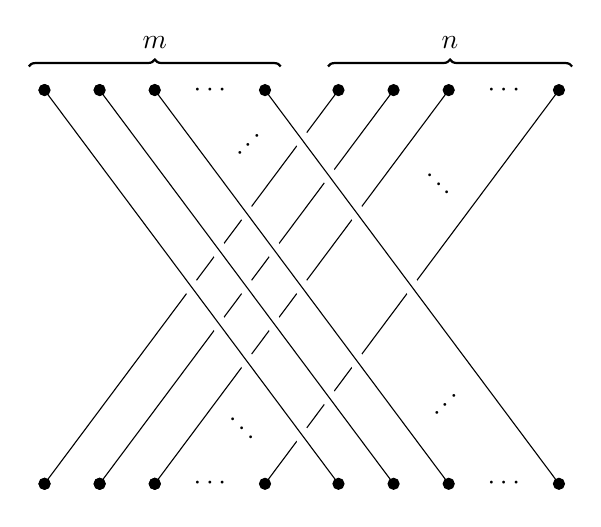
\begin{tikzpicture}
            \tikzset{
                position label/.style={
                below = 3pt,
                text height = 2ex,
                text depth = 1ex
                }
            }
            % \draw[thick] (-0.2,0) -- (6.7,0);
            % \draw[thick] (-0.2,-5) -- (6.7,-4);

            % draws the top two braces labeling m and n
            \draw[thick, decoration={brace}, decorate] (-0.2,0.3) -- (3,0.3);
            \draw[thick, decoration={brace}, decorate] (3.6,0.3) -- (6.7,0.3);
            \node at (1.4, 0.6) {$m$};
            \node at (5.15, 0.6) {$n$};
            
            % top second four points
            \foreach \x in {5.333, 6.333, 7.333}{
                \filldraw (\x*\ptsep, 0) circle (0.07cm); 
                \draw (\x*\ptsep,0) -- (\x*\ptsep - 5.333*\ptsep, -\height);
            }
            % ellipses
            \node at (8.333*\ptsep, 0) {$\cdots$};
            \filldraw (9.333*\ptsep,0) circle (0.07cm); % 8
            \draw (9.333*\ptsep,0) -- (9.333*\ptsep - \sep*\ptsep, -\height);

            % top first four points 
            \foreach \x in {0, 1, 2}{
                \filldraw (\x*\ptsep, 0) circle (0.07cm); % draws points
                \draw[line width = 2mm, white] (\x*\ptsep,0) -- (\x*\ptsep +\sep*\ptsep, -\height); % draws the strands
                \draw (\x*\ptsep,0) -- (\x*\ptsep +\sep*\ptsep, -\height); % draws the strands
            }
            %ellipses
            \node at (3*\ptsep, 0) {$\cdots$};
            \draw (4*\ptsep,0) -- (4*\ptsep + \sep*\ptsep, -\height);
            \draw[line width = 2mm, white] (4*\ptsep,0) -- (4*\ptsep + \sep*\ptsep, -\height);
            \draw (4*\ptsep,0) -- (4*\ptsep + \sep*\ptsep, -\height);
            \filldraw (4*\ptsep,0) circle (0.07cm); % 4 

            %%%%%%%%%%%%%%%%%%%%
            % draws the top and bottom points
            %%%%%%%%%%%%%%%%%
            \foreach \x in {0, 1, 2}{
                \filldraw (\x*\ptsep, 0) circle (0.07cm); 
            }

            \foreach \x in {0, 1, 2}{
                \filldraw (\x*\ptsep, -\height) circle (0.07cm); 
            }
            %ellipses
            \node at (3*\ptsep, -\height) {$\cdots$};
            \filldraw (4*\ptsep,-\height) circle (0.07cm); % 4 

            \foreach \x in {0, 1, 2}{
                \filldraw (\x*\ptsep, -\height) circle (0.07cm); 
            }

            % top second four points
            \foreach \x in {5.333, 6.333, 7.333}{
                \filldraw (\x*\ptsep, -\height) circle (0.07cm); 
            }
            % ellipses
            \node at (8.333*\ptsep, -\height) {$\cdots$};
            \filldraw (9.333*\ptsep,-\height) circle (0.07cm); % 8


            \node at (5,-1.2) {\rotatebox{-45}{$\cdots$}};
            \node at (2.5,-4.3) {\rotatebox{-45}{$\cdots$}};
            \node at (2.6,-0.7) {\rotatebox{45}{$\cdots$}};
            \node at (5.1,-4) {\rotatebox{45}{$\cdots$}};
        \end{tikzpicture}
    \end{figure}

    It is a simple exercise to show that this satisfies the hexagon axioms; 
    the task is simplified due to the fact that the associators are identities. 
    While this category may seem like a boring example, it plays a critical role 
    in demonstrating coherence for braided monoidal categories, something we will do later.
\end{example}

\begin{example}
    Let $\textbf{GrMod}_R$ be the category of graded $R$-modules 
    $M = \{M_n\}_{n = 1}^{\infty}$. Recall from 
    \ref{example_graded_R_modules} That $\textbf{GrMod}_R$ forms 
    a monoidal category.
    The tensor product 
    of two graded $R$ modules $M =\{M_n\}_{n=1}^{\infty}$ and $P = \{P_n\}_{n= 1}^{\infty}$ is the graded $R$-module $M\otimes P$ whose $n$-th level is given by
    \[
        (M \otimes P)_n = \bigoplus_{i + j = n}M_i \otimes P_j.
    \]  
    We can additionally introduce a braiding on this category for each invertible elements $k \in R$; specifically, we define the braiding 
    $\sigma_{M,P}: M \otimes P \to P \otimes M$ to be the graded module homomorphism whose $n$-th degree is 
    \begin{align*} 
        (\sigma_{M, P})_n: &\bigoplus_{i + j = n}M_i \otimes P_j
        \to 
        \bigoplus_{i + j = n} P_j \otimes M_i\\
        &(m \otimes p) \longmapsto k^{ij}p \otimes m
    \end{align*}
    whenever $m \in M_i$ and $p \in P_j$. 
    Observe that with this braiding we get that
    \begin{center}
        \begin{tikzcd}[row sep = 0.25cm, column sep = 0.5cm]
            &
            m \otimes (p \otimes q)
            \arrow[r, mapsto]
            &
            r^{(j + k)i}(p \otimes q) \otimes m
            \arrow[dr, mapsto]
            &
            \\
            (m \otimes p)\otimes q
            \arrow[ur, mapsto]
            \arrow[dr, mapsto]
            &
            &
            &
            \parbox{3.2cm}{
            \centering
            ${r^{(j + k)i}p\otimes (q \otimes m)}$\\
            $=$\\
            ${r^{ij}p\otimes(r^{ik}m \otimes q)}$
            }
            \\
            &
            r^{ij}(p\otimes m)\otimes q
            \arrow[r, mapsto]
            &
            r^{ij}p\otimes(m \otimes q)
            \arrow[ur, mapsto]
            &
        \end{tikzcd}
    \end{center}
    which clearly commutes. The second hexagon axiom is also easily seen to be satisfied:
    \begin{center}
        \begin{tikzcd}[row sep = 0.25cm, column sep = 0.5cm]
            &
            (m \otimes p) \otimes q
            \arrow[r, mapsto]
            &
            r^{(i + j)k}q\otimes(m \otimes p)
            \arrow[dr, mapsto]
            &
            \\
            m \otimes (p\otimes q)
            \arrow[ur, mapsto]
            \arrow[dr, mapsto]
            &
            &
            &
            \parbox{3.2cm}{
            \centering
            $r^{(i+j)k}(p\otimes m)\otimes n$\\
            $=$\\
            $r^{jk}(r^{ik}p \otimes m) \otimes n$
            }
            \\
            &
            r^{jk} m\otimes (q\otimes p)
            \arrow[r, mapsto]
            &
            r^{jk}(m\otimes q)\otimes p
            \arrow[ur, mapsto]
            &
        \end{tikzcd}
    \end{center}
    Thus we see that $\textbf{GrMod}_R$ is more than just a monoidal category; each invertible 
    element of $R$ induces a braiding, making it a braided monoidal category as well.
\end{example}

\begin{example}
    If $M$ is monoidal, we can recall from 
    Example \ref{example_monoidal_functor_category} that the functor category 
    $\cc^M$ is also monoidal. If additionally we have that $M$ is braided with 
    a braiding $\sigma_{A,B}: A\otimes B \to B \otimes A$,
    then we can extend this to a braiding on the functor category of $\cc^M$ 
    by defining, for two functors $F,G: \cc \to M$, the natural transformation
    \[
        \beta_{F,G}: F \otimes G \to G \otimes F 
    \] 
    defined pointwise for each $A \in \cc$ as the morphism
    \[
        (\beta_{F,G})_A = \sigma_{F(A), G(A)}: F(A)\otimes G(A) \isomarrow G(A) \otimes F(A). 
    \]
    One can then check that this natural transformation satisfies the braided hexagon 
    axioms since the braiding $\sigma$ in $M$ does, so that $\cc^M$ is additionally braided 
    if $M$ is additionally braided. 
\end{example}

\begin{definition}
    A \textbf{Symmetric Monoidal Category} $\cc$ is a braided monoidal category 
    such that, for the twist morphism, 
    \[
        \sigma_{B,A}\circ\sigma_{A,B} = 1_{A\otimes B}.
    \] 
\end{definition}

Symmetric monoidal categories are basically monoidal categories which collapse the 
information which braided monoidal categories have the potential to encode. 
Their environment is much simpler, but at the cost of information.

\begin{example}
    Recall from the previous examples that $\textbf{GrMod}_R$ can be treated 
    as a braided monoidal category. A braiding is given an invertible element 
    $r \in R$. However, consider the idempotent elements of this ring, i.e., the 
    elements $r \in R$ such that $r^2 = 1$. Then we see that these elements not only give 
    rise to braidings
    \begin{align*} 
        (\sigma_{M, P})_n: &\bigoplus_{i + j = n}M_i \otimes P_j
        \to 
        \bigoplus_{i + j = n} P_j \otimes M_i\\
        &(m \otimes p) \longmapsto k^{ij}p \otimes m
    \end{align*}
    but these braidings have the property that $\sigma_{M,P}\circ \sigma_{P,M} = 1_{M\otimes P}$, 
    since $r=1$.
    Hence the category of graded modules may be specially treated as symmetric monoidal categories 
    whenever there is an idempotent element of the ring $R$.
\end{example}

\begin{example}
    Recall from \ref{example:permutation_category} that the permutation category 
    $\mathbb{P}$ forms a monoidal category where objects are nonnegative integers and 
    homsets are given by the symmetric groups. The monoidal product $\otimes$ 
    simply sums the object, while two permutations $\tau \in S_n$ and $\rho\in S_m$
    are sent to the direct sum permutation $\tau\otimes \rho \in S_{n+m}$ (this permutation 
    simply horizontally stacks). 

    In this category, we can introduce a symmetric braiding $\sigma_{n,m}: n+m \to m+n$
    to be the unique permutation $\sigma_{n,m} \in S_{n+m}$ pictured below. 
    \begin{center}
        \begin{tikzcd}
            (\textcolor{red}{1}, \textcolor{red}{2}, \dots, \textcolor{red}{n}, \textcolor{blue}{n+1}, \textcolor{blue}{n + 2}, \dots, \textcolor{blue}{n+m})
            \arrow[d, "\sigma_{n,m}"]
            \\  
            (\textcolor{blue}{n + 1}, 
            \textcolor{blue}{n+2}, \dots, 
            \textcolor{blue}{n+m}, 
            \textcolor{red}{1}, 
            \textcolor{red}{2}, \dots, \textcolor{red}{n})
        \end{tikzcd}
    \end{center}
    One thing to notice is that this is the underlying permutation of braid given in 
    Figure \ref{figure:braiding_on_braid_category}.
    With the existence of this element of $S_{n+m}$ for every pair of objects 
    $n,m$ in $\mathbb{P}$, we see that the permutation category is actually symmetric monoidal.
\end{example}

\begin{definition}
    A \textbf{PROP}, an acronym coined by Mac Lane 
    for "Product and Permutation Category", 
    is a symmetric monoidal category $\mathbb{P}$ containing 
    the category $(\mathbb{N}, 0, +)$. 
\end{definition}

\begin{example}
    Consider the category $\textbf{FinSet}$, where the objects 
    are natural numbers $n$ and a morphism $f: n \to m$ is a function 
    from a set of size $n$ to one of size $m$. 

    Here, we necessarily include $0$ as an object; this denotes the empty set. 
    First we demonstrate that this is monoidal. 
    Let $n, m$ be any integers. Then we'll show that $+: \textbf{FinSet}\times\textbf{Finset} \to \textbf{FinSet}$ 
    is a bifunctor. First, we acknowledge that $n + m \in \textbf{FinSet}$. 

    Next, consider the set of morphisms
    \begin{align*}
        h&: k \to n \qquad f: n \to n'\\
        j&: l \to m \qquad g: m \to m'.
    \end{align*}
    Let $S_k$ be the set of $k$ elements. Now since $f, g$ are functions, 
    we know that $f: S_n \to S_{n'}$ and $g: S_m \to S_{m'}$ for some sets in 
    \textbf{Set}.Then we can define $f + g: (n + n') \to (m + m')$ to be the function 
    in \textbf{Set} where 
    \[
        f + g: S_n \amalg S_{n'} \to S_m \amalg S_{m'}.
    \]
    where 
    \[
        (f + g)(x, i) = 
        \begin{cases}
            (f(x), 0) \quad \text{ if } i = 0\\
            (g(x), 1) \quad \text{ if } i = 1.
        \end{cases}
    \]
    Hence $f + g$ makes sense in \textbf{FinSet} as morphism $f + g: (n + n') \to (m + m')$. 

    Now consider the morphisms $f \circ h$ and $g \circ j$. Observe that 
    $f\circ h + g \circ j : k + l \to n' + m'$. This is then the function 
    \[
        f\circ h + g \circ j: S_k \amalg S_{l} \to S_{n'} \amalg S_{m'}
    \]
    but note that 
    \begin{align*}
        f\circ h + g \circ j: S_k \amalg S_{l} \to S_{n'} \amalg S_{m'}
        =   
        (f + g)\circ(h + j)
    \end{align*}
    Hence we must have that $(f + g)\circ(h + j) = f\circ h + g \circ j$, so that 
    we have that $+$ is a bifunctor. 

    Now we show that this is a monoidal category. Define the natural isomorphisms 
    \begin{align*}
        \alpha_{n,m,p} &: n + (m + p) \isomarrow (n + m) + p\\
        \lambda_n &: 0 + n \isomarrow n\\
        \rho_n &: n + 0 \isomarrow n.
    \end{align*}
    We can describe these functions in further detail. 
    Observe that $\alpha_{n, m, p}$ can be realized to be a function where 
    \[
        \alpha_{n,m,p}: S_n\amalg(S_m \amalg S_p) \isomarrow (S_n \amalg S_m)\amalg S_p.
    \]
    Elements of $S_n \amalg(S_m \amalg S_p)$ will be either $(x, 0)$ 
    where $x \in S_n$, or $(x, 1)$ where $x \in S_m\amalg S_p$. In turn, the elements 
    of this set are of the form $(y, 0)$ where $y \in S_m$ and $(y, 1)$ where 
    $y \in S_p$. 
    
    On the other hand, elements of $(S_n \amalg S_m)\amalg S_p$ are of the form 
    $(x', 0)$ if $x' \in S_n \amalg S_m$ or are of the form $(x', 1)$ if $x' \in S_p$. 
    Furthermore, elements of $S_n\amalg S_m$ are of the form $(y', 0)$ if $y' \in S_n$ \
    and $(y', 1)$ if $y' \in S_m$.

    Now we can explicitly define $\alpha_{n,m,p}$ as 
    \begin{align}
        \alpha_{n,m,p}(x, i) = 
        \begin{cases}
            ((x, 0), 0) \qquad &\text{ if } i = 0\\
            ((y, 1), 0) \qquad &\text{ if } i = 1 \text{ and } x = (y, 0)\\
            (y, 1) \qquad &\text{ if } i = 1 \text{ and } x = (y, 1)
        \end{cases}
    \end{align}
    and $\lambda$ as 
    \begin{align*}
        \lambda_n(x, 1) = x
    \end{align*}
    and $\rho$ as 
    \begin{align*}
        \rho_n(x, 0) = x.
    \end{align*}
    Note for both $\lambda$ and $\rho$, there is only one case for $(x ,i)$ since 
    for $\lambda$, $i$ is never $0$ and for $\rho$, $i$ is never 1.  

    All of these establish a bijection, and hence an isomorphism. 
    Now to demonstrate that they are natural, consider $f: n \to n'$, 
    $g: m \to m'$ and $h: p \to p'$.
    First, we'll want to show that the diagram 
    \begin{center}
        \begin{tikzcd}[row sep = 1.4cm, column sep = 1.4cm]
            n + (m + p) 
            \arrow[r, "\alpha_{n,m,p}"] 
            \arrow[d, swap, "f + (g + h)"]
            & 
            (n + m) + p
            \arrow[d, "(f + g) + h"]\\
            n' + (m' + p')
            \arrow[r, swap, "\alpha_{n', m', p'}"]
            &
            (n' + m') + p'
        \end{tikzcd}
    \end{center}
    commutes, which we can do by a case-by-case basis.
    First we follow the path
    \begin{align*}
        [(f + g) + h] \circ \alpha_{n, m, p}: 
        S_n\amalg(S_m \amalg S_p) \to (S_{n'}\amalg S_{m'})\amalg S_{p'}.
    \end{align*}
    and then show it is equivalent to the other path.
    \begin{description}
        \item[$\bm{i = 0}$]
        If the input is $(x, 0)$, we see that $\alpha_{n,m,p}(x, i) = ((x,0),0)$.
        If this is fed into $(f + g) + h$, the output will be $(f + g)(x, 0)$, whose output 
        will be $((f(x), 0), 0)$. 

        However, suppose we first put $(x, 0)$ into $f+ (g + h)$. Then 
        we would have directly obtain $(f(x), 0)$. Feeding this into $\alpha_{n', m', p'}$, we would 
        get $((f(x), 0), 0)$. Hence we obtain naturality in this case. 

        \item[$\bm{i = 1}$.]
        Suppose now the input is $(x, 1)$. Then either $x = (y, 0)$ with $y \in S_m$ 
        or $(y, 1)$ where $y \in S_p$. 

        \begin{description}
            \item[$\bm{y \in S_m}$.] Suppose $x = (y, 0)$. Then we see that 
            $\alpha_{n,m,p}(x, 1) = ((y, 1), 0)$. Plugging this into $( f+ g) + h$, we 
            get 
            \[
                [ ( f+ g) + h]((y, 1), 0) = ([f + g](y, 1), 0) = ((g(y), 1), 0).
            \]
            However, we also could have obtained this value by first starting with  
            $f + (g + h)$. In this case, 
            \[
                [f + (g + h)]((y, 0), 1) = ([g + h](y, 0), 1) = ((g(y), 0), 1). 
            \]
            Plugging this into $\alpha_{n',m',p'}$, we then get that 
            \[
                \alpha_{n',m',p'}((g(y), 0), 1) = ((g(y), 1), 0).
            \]
            Hence the two paths are equivalent. 

            \item[$\bm{y \in S_p}$.] Suppose $x = (y, 1)$, Then we have that 
            $\alpha_{n, m, p}((y,1), 1) = (y, 1)$. Sending this into $(f + g)+ h$, we get 
            \[
                [(f + g) + h](y, 1) = (h(y), 1).
            \]
            However, we could have achieved this value by first plugging $((y, 1),1)$ into 
            $f + (g + h)$:
            \[
                [f + (g + h)]((y, 1), 1) = ([g + h](y, 1), 1) = ((h(y), 1), 1).
            \]  
            Then sending this into $\alpha_{n',m',p'}$, we get 
            \[
                \alpha_{n',m',p'}((h(y), 1), 1) = (h(y), 1).
            \]
            Thus the two paths are equivalent.
        \end{description}
        Hence we see that this diagram does commute, so that $\alpha$ is natural. 
    \end{description}
    [Show naturality works for $\lambda$ and $\rho$.]

    Now we show that these natural isomorphisms satisfy the monoidal properties. 
    Specifically, we'll show that the diagram 
    \begin{center}
        \begin{tikzcd}[row sep = 1.4cm, column sep = 1.4cm]
            n + (0 + m) \arrow[rr, "\alpha_{n, 0, m}"]
            \arrow[dr, swap, "1_n + \lambda_m"]
            &
            &
            (n + 0) + m 
            \arrow[dl, "\rho_n + 1_m"]\\
            &
            n + m
            &
        \end{tikzcd}.
    \end{center}
    must commute. To do this, we consider how these functions are realized in \textbf{Set}. 
    If we consider $(x, i) \in S_n\amalg(\varnothing \amalg S_m)$, we see that 
    we have two cases to consider. 
    \begin{description}
        \item[$\bm{i = 0}$.]
        If $i = 0$, then we see that $\alpha_{n, 0, m}(x, 0) = ((x, 0), 0)$. Sending 
        this into $\rho_n + 1_m$, we get that $[\rho_m + 1_m]((x, 0), 0) = (\rho(x, 0), 0) = (x, 0)$. 

        On the other hand, we could obtain this value by directly sending $(x, 0)$ into 
        $1_n + \lambda_m$. Observe that $[1_n + \lambda_m](x, 0) = (1_n(x), 0) = (x, 0)$. 
        Hence the diagram commutes for this case. 

        \item[$\bm{i = 1}$.] If $i = 1$, then our element is of the form 
        $(x, 1)$. However, we know that $x = ((x, 1), 0)$, since $(x, 1) \in 0 + m$. 
        Thus observe that $\alpha_{n, 0, m}((x, 1), 1) = (x, 1)$. Consequently, 
        we get that $[\rho_n + 1_m](x, 1) = (1_m(x), 1) = (x, 1)$. 

        On the other hand, we can start instead be evaluating 
        $[1_n + \lambda_m]((x, 1), 1) = (\lambda(x, 1), 1) = (x, 1)$. Hence the diagram commutes 
        in this case.
    \end{description}
    Thus we see that this diagram holds for all naturals $n, m$.
\end{example}

\newpage
\section{Coherence for Braided Monoidal Categories}
We saw with monoidal categories that ultimately everything we were saying \emph{made sense}. 
That is, we saw that our definition does not give us an contradictions, and that we 
can obtain a significant coherence result which ultimately allows us to not worry 
about the particular parenthesization of a monoidal product. Further, we saw that 
diagrams freely built from associators and unitors were all commutative. 

With braided monoidal categories we can get a similar statement. This time, however, 
it is a bit weaker, although it is nevertheless extremely useful. It was Joyal and Street 
in the 1993 paper who both first proved the coherence for braided monoidal categories. 
Their work heavily relies on the work of G.M. Kelly, and they use very slick, 
higher categorical tricks.
 
In this section, we spell out those tricks. 

\begin{definition}[Joyal-Street]
    Let $\aa$ be a category with $\vv$ a monoidal category. Suppose $T: \aa \to \vv$ is a functor.
    We define a \textbf{Yang-Baxter operator}
    to be a family of isomorphisms
    \[
        y_{A,B}: T(A)\otimes T(B) \isomarrow T(B) \otimes T(A).
    \]
    for each $A, B \in \aa$ such that the diagram below commutes.
    such that the diagram below commutes.
\end{definition}

\begin{center}
\begin{tikzcd}[row sep = 1cm]
    &[-3cm]
    T(A) \otimes T(B) \otimes T(C) 
    \arrow[dl, swap, "1 \otimes B_{B,C}"]
    \arrow[r, "y_{A,B} \otimes 1"]
    &[0.8cm]
    T(B) \otimes T(A) \otimes T(C)
    \arrow[dr, "1\otimes y_{A,C}"]
    &[-3cm]
    \\
    T(A)\otimes T(C) \otimes T(B)
    \arrow[dr, swap, "y_{A,C} \otimes 1"]
    &
    &
    &
    T(B) \otimes T(C) \otimes T(A)
    \arrow[dl, "y_{B,C} \otimes 1"]
    \\
    &
    T(C) \otimes T(A) \otimes T(B)
    \arrow[r, swap, "1 \otimes y_{A,B}"]
    &
    T(C) \otimes T(B) \otimes T(A)
    &
\end{tikzcd}
\end{center}

Note that here we omit the associators although they are implicitly included in the diagram. 
Note also that, for any functor 
$T: \aa \to \vv$ with $\vv$ a braided monoidal category,
$T$ trivially has a Yang-Baxter operator $y$ where we set 
\[
    y_{A,B} = \sigma_{T(A),T(B)}.
\]
Before we move forward we introduce a notion that can be found in \cite{Joyal1993BraidedTC}, originally from \cite{kelly_clubs}.
For our purposes, we will denote the category obtained via disjoint unions of the symmetric groups $S_n$ as $\mathbb{P}$. That is, the objects of $\mathbb{P}$ are natural numbers and 
\[
    \hom_{\mathbb{P}}(n,m)
    =
    \begin{cases}
        S_n & \text{if } n = m\\
        \varnothing & \text{if } n \ne m 
    \end{cases}
\]

\begin{definition}
   Let $\aa$ be a category and suppose suppose $\dd \in \textbf{Cat}/\mathbb{P}$. That is, $\dd$ is a category with an associated functor
   $\Gamma: \dd \to \mathbb{P}$. Then we define the category $\dd\int\aa$ where 
    \begin{description}
        \item[Objects.] Finite strings $[A_1, A_2, \dots, A_n]$ with $A_i \in \aa$
        \item[Morphisms.] For two strings $[A_1, \dots, A_n]$ and $[B_1, \dots, B_n]$, denoted as $[A_i]$ and $[B_i]$,
        \[
            \hom_{\dd\int\aa}\Big([A_i],[B_i]\Big)
            =
            \Big\{(\alpha, f_1, \dots, f_n) \mid f_i \in \hom_{\aa}(A_i, B_{\sigma(i)})  \Big\}
        \]
        Here $\alpha$ is a morphism of $\dd$ such that $\Gamma(\alpha) = \sigma \in S_n$.
        Finally, we allow no morphisms between two different strings of different length.
    \end{description}
\end{definition}
For any category $\aa$, there exists a natural inclusion functor 
\begin{gather*}
    i_{\aa}: \aa \to \dd\int\aa\\
    i_{\aa}(A) = [A]
    \qquad
    i_{\aa}(f: A \to B) = (e_1,f) : [A] \to [B]
\end{gather*}
where $e_1$ is the sole element of $S_1$. This functor will be useful for us later.
Next we formalize the following category which can be thought of as a generalized functor category. 

\begin{definition}
    Let $\aa, \bb$ be categories.
    Denote the category $\{\aa, \bb\}$
    as the category with objects $(n, F: \aa^n \to \bb)$ 
    whose morphisms are 
    \[
        \hom_{\{\aa, \bb\}}\Big((n, T), (m,S)\Big)
        =
        \begin{cases}   
            \{(\sigma, \eta: \sigma\cdot T \to S) \} & \text{if } n = m\\
            \varnothing & \text{if } n \ne m.
        \end{cases}
    \]
    Here $\sigma \in S_n$, and $\eta: \sigma \cdot T \to S$ is a natural transformation from the functor $\sigma \cdot T$ defined pointwise as 
    \[
        \sigma \cdot T(A_1, A_2, \dots, A_n)
        =
        T(A_{\sigma(1)}, \dots, A_{\sigma(n)})
    \]
    to the functor $S$. 
\end{definition}


    There are two things we need to say about this category.
    First, for any generalized functor category $\{\aa, \vv\}$, there exists a a projection functor 
    $\Gamma: \{\aa, \bb\} \to \mathbb{P}$ defined on objects and morphisms as
    \begin{gather*}
        \Gamma(n, T: \aa^n \to \bb) = n 
        \qquad 
        \Gamma(\sigma, \eta: \sigma\cdot T \to S)
        = 
        \sigma.
    \end{gather*}
    Hence we see that each category $\{\aa, \bb\}$ is actually a member of $\textbf{Cat}/\mathbb{P}$, because it always comes equipped with a functor into $\mathbb{P}$.
    
    Second, if $\vv$ is a strict monoidal category, then so is $\{\aa, \vv\}$. One can see this by defining for 
    two functors $T: \aa^n \to \vv$ and $S: \aa^m \to \vv$ the functor
    $T \otimes S: \aa^{n+m} \to \vv$ which is a functor that can be defined pointwise as 
    \[
        (T \otimes S)(A_1, \dots, A_{n+m}) = T(A_1, \dots, A_n)\otimes S(A_{n+1}, \dots, A_{n+m}).
    \]
    Thus if $\vv$ is strict, then so it $\{\aa, \vv\}$.

What is useful about this construction is that 
Kelly showed that the functors 
\[
    (-)\int A : \textbf{Cat}/\mathbb{P} \to \textbf{Cat} 
    \qquad 
    \{A, (-) \}: \textbf{Cat}\to \textbf{Cat}/\mathbb{P}
\]
form an adjunction. 
We use this in the next proposition, which is also aided by the following lemma. 

\begin{lemma}
    Let $\vv$ be a strict monoidal category. 
    Suppose $T: \textbf{1} \to \vv$ has a Yang-Baxter operator
    $y$. Then there exists a
    unique strict monoidal functor $T': \mathbb{B} \to \vv$ such that the diagram below commutes. 
    \begin{center}
        \begin{tikzcd}[column sep = 1.4cm, row sep = 1cm]
            \mathbf{1} \arrow[r, "i"]
            \arrow[dr, swap, "T"]
            &
            \mathbb{B}
            \arrow[d, dashed, "T'"]
            \\
            &
            \vv
        \end{tikzcd}
    \end{center}
    Further, we have that $T'(\sigma) = y$.
\end{lemma}

\begin{proof}
    Denote the element of $\mathbf{1}$ as $\bullet$. Then
    $T(\bullet) = X$ for some $X \in \vv$. Towards a definition of $T'$, let 
    $T': \mathbb{B} \to \vv$ 
    be defined on objects as $T'(1) = X$. If we force $T'$ to be strict, 
    this will define its value on all objects of 
    $\mathbb{B}$. On morphisms, first observe that 
    each $\beta \in B_n$ can be expressed in terms of its 
    generators $\sigma_i$. Hence it suffices to define the action of 
    $T'$ on a generator $\sigma_i$, and we do this naturally as:
    \begin{align*}
        T'(\sigma_i) &= 1_X^{\otimes(i-1)}\otimes y_{X,X}\otimes 1_X^{\otimes(n-i-1)}: X^{\otimes n} \to X^{\otimes n}
    \end{align*}
    We then define $T'(\beta)$ as the iterative composite over the generators. 
    We are then left to check that the relations of $\mathbb{B}$ are preserved (which they are). 
    This then allows us to define $T': \mathbb{B} \to \vv$ to be a unique, well defined strict 
    monoidal functor which allows the diagram to commute.
\end{proof}

\begin{proposition}\label{proposition:triangle_commutes}
    Let $\vv$ be a strict monoidal category, and suppose we have a
    functor $T: \aa \to \vv$ with associated Yang-Baxter operator
    $y$. Let $z$ be the Yang-Baxter operator on $i_{\aa}: \aa \to \mathbb{B}\int\aa$.
    Then there exists a unique strict monoidal functor $T': \mathbb{B}\int\aa \to \vv$ such that the diagram
    \begin{center}
        \begin{tikzcd}[column sep = 1.4cm, row sep = 1cm]
            \aa \arrow[r, "i_{\aa}"]
            \arrow[dr, swap, "T"]
            &
            \mathbb{B}\int\aa
            \arrow[d, dashed, "T'"]
            \\
            &
            \vv
        \end{tikzcd}

    \end{center}
    commutes and that $T'(y') = y$. 
\end{proposition}

\begin{proof}
    Recall that $\{\aa, \vv\}$ is a strict monoidal category if $\vv$ is. Consider again the one point category $\mathbf{1}$ and construct functors $F_S: \mathbf{1} \to \{\aa, \vv\}$ 
    and
    $j: \mathbf{1} \to  \mathbb{B}$
    where $F_T(\bullet) = T: \aa \to \vv$ and $i(\bullet) = 1$. Then by the previous work,
    there exists a map $T^{\#}: \mathbb{B} \to \{\aa, \vv\}$ such that the diagram below commutes.
    \begin{center}
        \begin{tikzcd}[column sep = 1.4cm, row sep = 1cm]
            \mathbf{1} \arrow[r, "i"]
            \arrow[dr, swap, "F_T"]
            &
            \mathbb{B}
            \arrow[d, dashed, "T^{\#}"]
            \\
            &
            \{\aa, \vv\}
        \end{tikzcd}
    \end{center}
    
    Now construct the maps $\{F_S\}: \{*\} \to \hom(\mathbf{1}, \{\aa, \vv\})$ and $\{S\}: \{*\} \to \hom (\aa, \vv)$ where $\{F_S\}(*) = F_S$ and $\{S\}(*) = S$. Consider the pullback squares below. 
    \begin{center}
        \begin{tikzcd}[column sep = 0.8cm, row sep = 1cm]
            P
            \arrow[r]
            \arrow[d]
            &
            \hom (\mathbb{B}, \{\aa, \vv\})
            \arrow[d, "(-) \circ i"]
            \\
            \{*\}
            \arrow[r, swap, "\{F_S\}"]
            &
            \hom (\mathbf{1}, \{\aa, \vv\})
        \end{tikzcd}
        \begin{tikzcd}[column sep = 0.8cm, row sep = 1cm]
            (K, T)
            \arrow[r, maps to]
            \arrow[d, maps to]
            &
            T:\mathbb{B} \to \{\aa, \vv\}
            \arrow[d, maps to]
            \\
            *
            \arrow[r, maps to]
            &
            F_S = T \circ i
        \end{tikzcd}
    \end{center}
    
    \begin{center}
        \begin{tikzcd}[column sep = 0.8cm, row sep = 1cm]
            Q
            \arrow[r]
            \arrow[d]
            &
            \hom (\mathbb{B}\int\aa, \vv)
            \arrow[d, "(-) \circ i_A"]
            \\
            \{*\}
            \arrow[r]
            &
            \hom (\aa, \vv)
        \end{tikzcd}
        \begin{tikzcd}[column sep = 0.8cm, row sep = 1cm]
            (K', T')
            \arrow[r, maps to]
            \arrow[d, maps to]
            &
            T':\mathbb{B} \to \{\aa, \vv\}
            \arrow[d, maps to]
            \\
            *
            \arrow[r, swap, "\{S\}", maps to]
            &
            S = T' \circ i_A
        \end{tikzcd}
    \end{center}
    First, $P$ corresponds to the set of functors $T: \mathbb{B} \to \{\aa, \vv\}$ such that precomposition with $i$ is equal to $F$. Meanwhile, the set $Q$ consists of functors $T': \mathbb{B}\int\aa \to \vv$ where precomposition with $i_{\aa}$ is equal to $S$. However, these sets are in bijection due to the adjoint relation we have. In other words, the diagrams 
    \begin{center}
        \begin{tikzcd}[column sep = 1.4cm, row sep = 1cm]
            \mathbf{1} \arrow[r, "i"]
            \arrow[dr, swap, "F_S"]
            &
            \mathbb{B}
            \arrow[d, dashed, "T"]
            \\
            &
            \{\aa, \vv\}
        \end{tikzcd}
        \begin{tikzcd}[column sep = 1.4cm, row sep = 1cm]
            \aa \arrow[r, "i_{\aa}"]
            \arrow[dr, swap, "S"]
            &
            \mathbb{B}\int\aa
            \arrow[d, dashed, "T'"]
            \\
            &
            \vv
        \end{tikzcd}
    \end{center}
    are in bijection. Hence we see that $T^{\#}$
    corresponds uniquely with a functor $T'$ such that 
    the diagram 
    \begin{center}
        \begin{tikzcd}[column sep = 1.4cm, row sep = 1cm]
            \aa \arrow[r, "i_{\aa}"]
            \arrow[dr, swap, "T"]
            &
            \mathbb{B}\int\aa
            \arrow[d, dashed, "T'"]
            \\
            &
            \vv
        \end{tikzcd}
    \end{center}
    commutes and preserves the Yang-Baxter operators as desired. 
\end{proof}

\begin{theorem}
    Let $\vv$ be an $B$-category and suppose we have a functor $F: \aa \to \vv$. Then there is an equivalence of categories 
    \[
       \mathbb{B}\text{\emph{Fun}}(\mathbb{B}{\textstyle\int}\aa, \vv) \simeq \text{\emph{Fun}}(\aa, \vv).
    \]
    given by precomposition of each $F: \mathbb{B}\int\aa \to \vv$ with $i_{\aa}: \aa \to \mathbb{B}\int\aa$.
\end{theorem}

\begin{proof}
    We follow the same argument as Joyal and Street. By the previous lemma, every $SB$-monoidal category is strongly equivalent to a strict $SB$-monoidal category $\vv'$ via a pair of functors $E: \vv \to \vv'$ and $E': \vv' \to \vv$. Hence observe that if we have an equivalence of categories $(-) \circ i_{\aa}: \mathbb{B}\fun(\mathbb{B}\int\aa, \vv') \to \fun(\aa, \vv')$, then the diagram below commutes
     \begin{center}
         \begin{tikzcd}[column sep = 1.4cm, row sep = 1.4cm]
             \mathbb{B}\text{Fun}(\mathbb{B}{\textstyle\int}\aa, \vv)
             \arrow[r, "(-) \circ i_{\aa}", dashed]
             \arrow[d, swap, "F \circ (-)"]
             &
             \text{Fun}(\aa, \vv)
             \\
             \mathbb{B}\text{Fun}(\mathbb{B}{\textstyle\int}\aa, \vv')
             \arrow[r, swap, "(-) \circ i_{\aa}"]
             &
             \text{Fun}(\aa, \vv')
             \arrow[u,swap, "E' \circ (-)"]
         \end{tikzcd}
     \end{center}
    and the top dashed arrow is an equivalence as well.
    So it suffices to prove this for the strict case. 
    Now, the proposed functor $F$ behaves as 
    \[
        F(S: \mathbb{B}\int\aa \to \vv) = S \circ i_{\aa}: \aa \to \vv.
    \]
    We must demonstrate that this is fully faithful and essentially surjective.
    \begin{description}
        \item[Fully faithful.]
        Let $F, G: \mathbb{B}\int\aa \to \vv$ be strong $SB$-monoidal functors. Then define the function
        \[
            \phi: \hom_{\mathbb{B}\text{Fun}(\mathbb{B}{\textstyle\int}\aa, \vv)}(F,G)
            \to 
            \hom_{\text{Fun}(\aa, \vv)}(F \circ i_{\aa}, 
            G\circ_{i_{\aa}}).
        \]
        where, given a natural transformation $\eta: F \to G$,
        we have that $\phi(\eta): F\circ i_{\aa} \to G \circ i_{\aa}$ is a natural transformation defined as 
        \[
            \phi(\eta)_A = \eta_{[A]}.
        \]
        We show that this is injective. Suppose $\phi(\eta) = \phi(\eta')$ for two natural transformations $\eta, \eta': F \to G$ with $F, G \in \mathbb{B}\text{Fun}(\mathbb{B}\int\aa, \vv)$.
        The fact that $\phi(\eta) = \phi(\eta')$ implies that 
        \[  
            \eta_{[A]} = \eta_{[A']}.
        \]
        As these are natural transformations between monoidal functors, we have that the diagram below commutes. 
        \begin{center}
            \begin{tikzcd}[column sep = 2cm, row sep = 1.4cm]
                F([A_1])\otimes \cdots \otimes 
                F([A_n])
                \arrow[r, "\eta_{[A_1]}\otimes \cdots \otimes \eta_{[A_n]}"]
                \arrow[d, "\cong", "P_1"']
                &
                G([A_1])\otimes \cdots \otimes 
                G([A_n])
                \arrow[d, "P_2", "\cong"']
                \\
                F([A_1, \dots, A_n])
                \arrow[r, swap, "\eta_{[A_1, \dots, A_n]}"]
                &
                G([A_1, \dots, A_n])
            \end{tikzcd}
        \end{center}
        The morphisms $P_1$ and $P_2$ are the isomorphisms built inductively from 
        \[
            F_2: F([A]) \otimes F([B] \isomarrow F([A, B])
        \]
        which comes equipped with the data of a strong monoidal functor [see Mac Lane, p. 256]. Moreover, the diagram commutes by Mac Lane's coherence theorem. 
        
        The above diagram similarly holds with $\eta$ replaced as $\eta'$, since $\eta'$ is also a natural transformation of monoidal functors. Hence what we see is that 
        \begin{align*}
            \eta_{[A_1, \dots, A_n]} \circ P_1
            &= 
            P_2 \circ \eta_{[A_1]}\otimes \cdots \otimes \eta_{[A_n]}\\
            &=
            P_2 \circ \eta'_{[A_1]}\otimes \cdots \otimes \eta'_{[A_n]}\\
            &=
            \eta'_{[A_1, \dots, A_n]} \circ P_1.
        \end{align*}
        As $P_1$ is an isomorphism, we have that $\eta_{[A_1, \dots, A_n]} = \eta'_{[A_1, \dots, A_n]}$, so that 
        $\phi(\eta) = \phi(\eta')$ implies that $\eta = \eta'$. Hence the functor is faithful. The functor is clearly full, since  by the above process we can always take a natural transformation $\eta: F\circ i_{\aa} \to G\circ i_{\aa}$ and build it into a natural transformation $\eta: F \to G$. 
        
    \item[Essentially Surjective.]
        Consider a functor $F: \aa \to \vv$. 
        By Proposition \ref{proposition:triangle_commutes}, we know there exists 
        a unique $S: \mathbb{B}\int\aa \to \vv$ such 
        that $S \circ i_{\aa} = F$. 
        Hence we have essential surjectivity; in fact, we have 
        a stronger version in the strict case.
    \end{description}
\end{proof}


\newpage
\section{Monoids, Groups, in Symmetric Monoidal Categories}
Recall from section ? that we were able to construct monoid and groups which 
were internal to some category $\cc$. The philosophy behind the construction 
is one we've seen before: we of course think of monoids and groups by their elements, 
but we resist the temptation and instead present an object-free, diagrammatic 
set of axioms for monoids and rings. We utilized the cartesian product in the 
category $\cc$ to demonstrate this. However, we now know that the cartesian 
product in any category is a small example of a category with a symmetric monoidal structure. 
Hence we revisit the concepts of a monoid and group, and expand their 
generality by demonstrating that they can be defined in a symmetric monoidal category. 

\begin{definition}
    Let $(\mathcal{M}, \otimes, I, \alpha, \rho, \lambda)$ 
    be a monoidal category and let $M$ be an object of $\mathcal{M}$.
    We say $M$ is if there exist maps 
    \begin{align*}
        \mu&: M\otimes M \to M \\
        \eta&: I \to M
    \end{align*}
    referred to as the multiplication and identity maps, such that the diagrams below 
    commute. 
    \begin{center}
        \begin{tikzcd}[column sep = 1.4cm, row sep = 1.4cm]
            M \otimes (M \otimes M) \arrow[r, "\alpha"]
            \arrow[d, swap, "1\otimes \mu"]
            &
            (M\otimes M)\otimes M
            \arrow[r, "\mu \otimes 1_M"]
            &
            M \otimes M
            \arrow[d, "\mu"]
            \\
            M \otimes M
            \arrow[rr, swap, "\mu"]
            &
            &
            M
        \end{tikzcd}

        \begin{tikzcd}[column sep = 1.4cm, row sep = 1.4cm]
            I \otimes M \arrow[r, "\eta \otimes 1_M"]
            \arrow[dr, swap, "\lambda_M"]
            &
            M \otimes M 
            \arrow[d, "\mu"]
            &
            M \otimes I \arrow[l, swap, "1_M \otimes \eta"]
            \arrow[dl, "\rho_M"]
            \\
            &
            M
            &
        \end{tikzcd}
    \end{center}
\end{definition}

\begin{example}
    One of the most useful examples of this concept arises from the notion of 
    an algebra $A$ over some field $k$, where $A$ is a vector space over the field 
    $k$. 
\end{example}

\newpage
\section{Enriched Categories}

When we originally defined categories, we sought a degree of large generality 
that was able to capture a huge amount of mathematical phenomenon. However, this 
was not out a mere desired for generality; as Mac Lane puts it, "good general theory
does not search for the maximum generality, but for the right generality" (108). 
But it does turn out that in defining categories so widely we lose some of their internal 
structure; for example, in many categories, every homset might have a underlying 
abelian group structure. These are called \textbf{preadditive categories} and are extremely 
useful, in that they give us a first step towards a general framework (but not to general) 
that allows one to do homological algebra in. 

Now if we've lost some original framework, how do we recover it? First, recall that 
in categories, objects are basically dummies. It doesn't matter how I denote my objects 
in my category $\cc$; you and are I talking about the same category if our morphisms 
act the same exact way. For example, the categories 
\begin{center}
    \begin{tikzcd}
        1 \arrow[r] \arrow[out=120,in=60,looseness=3,loop]
        &
        2 \arrow[r] \arrow[out=120,in=60,looseness=3,loop]
        &
        3 \arrow[r] \arrow[out=120,in=60,looseness=3,loop]
        &
        \cdots \arrow[r] 
        & 
        n \arrow[scale = 2.5, out=123,in=57,looseness = 3, loop]
    \end{tikzcd}
\end{center}
and 
\begin{center}
    \begin{tikzcd}
        \text{All} \arrow[r] \arrow[out=120,in=60,looseness=3,loop]
        &
        \text{Politicians} \arrow[r] \arrow[out=120,in=60,looseness=3,loop]
        &
        \text{Are} \arrow[r] \arrow[out=120,in=60,looseness=3,loop]
        &
        \cdots \arrow[r] 
        & 
        \text{Corrupt} \arrow[scale = 2.5, out=123,in=57,looseness = 3, loop]
    \end{tikzcd}
\end{center}
where the above objects are $n$ words describing how politicians suck,
are the same preorders. Thus, because categorical 
structure is primarily found within the morphisms, i.e. the homsets, we only need to 
fix these to take back our original structure. 

\begin{definition}
    Let $(\mathcal{V}, \otimes, I)$ be a monoidal category. A small category $\cc$ is a $\mathcal{V}$-category 
    or an \textbf{enriched category} over $\mathcal{V}$ if 
    \begin{itemize}
        \item[1.] For each $A, B \in \cc$, we have that $\hom_{\cc}(A, B) \in \mathcal{V}$ 
        \item[2.] There exists a "composition" operator 
        \[
            \circ_{A, B, C} : \hom_{\cc}(A, B) \times \hom_{\cc}(B, C) \to \hom_{\cc}(A, C)
        \]  
        \item[3.] For each object $A \in \cc$, we have a "identity object" 
        \[
            i_A: I \to \hom_{\cc}(A, A)  
        \] 
    \end{itemize}
    such that our composition operator is associative: 
    \begin{center}
        \begin{tikzcd}[row sep = 1.4cm, column sep = 0.5cm]
            \hom(A, B) \otimes (\hom(B, C) \otimes \hom(C, D))
            \arrow[d, swap, "1 \otimes \circ_{B, C, D}"]
            \arrow[rr, "\alpha"]
            &
            &
            (\hom(A, B) \otimes \hom(B, C))\otimes \hom(C, D)
            \arrow[d, "\circ_{A, B, C} \otimes 1"]
            \\
            \hom(A, B) \otimes \hom(B, D)
            \arrow[r, swap, "\circ_{A, B, D}"]
            &
            \hom(A, D)
            &
            \hom(A, C) \otimes \hom(C, D)
            \arrow[l, "\circ_{B, C, D}"]
        \end{tikzcd}
    \end{center}
    and such that our unital elements in each homset behave morally like an identity 
    element should:
    \begin{center}
        \begin{tikzcd}[row sep = 1.4cm, column sep = 1cm]
            \hom(B,B)\otimes \hom(A, B)
            \arrow[r, "\circ_{A, B, B}"]
            &
            \hom(A, B)
            &
            \hom(A, B)\otimes \hom(A, A)
            \arrow[l, swap, "\circ_{A, A, B}"]
            \\
            I \otimes \hom(A, B)
            \arrow[u, "i_B \otimes 1"]
            \arrow[ur, swap, "\lambda"]
            &
            &
            \hom(A, B)\otimes I
            \arrow[u, swap, "1\otimes i_A"]
            \arrow[ul, "\rho"]
        \end{tikzcd} 
    \end{center}
\end{definition}

\begin{example}
    The following is a classic example due to F.W. Lawvere.
    A \textbf{Lawvere metric space} is a set $X$ 
    equipped with a distance function $d: X\times X \to \rr$ such that 
    \begin{itemize}
        \item[1.] $d(x, x) = 0$ for all $x \in X$
        \item[2.] $d(x, z) \le d(x, y) + d(y, z)$ for all $x, y, z \in X$.  
    \end{itemize}
    It turns out that, we may equivalently define such a space as a category enriched 
    over $([0, \infty), +, 0)$.

    Recall that $([0, \infty), +, 0)$ where $+$ is addition forms a symmetric monoidal 
    category. Here we treat $[0, \infty]$ as a poset where for a pair of objects $a, b$ 
    there exists exactly one morphism 
    \[
        a \to b \text{ iff } b \le a.   
    \] 
    Now what does it look like for a category $\cc$ to be $[0, \infty]$-category? 
    It means that for any pair of objects $A, B$, we have that $\hom_{\cc}(A, B) \in [0, \infty)$.
    If we denote $d(A, B) = \hom_{\cc}(A, B)$,
    this then implies that we have a function 
    \[
        d: \ob(\cc)\times\ob(\cc) \to [0, \infty].
    \]
    Enriched categories also grant us a composition morphism
    \[ 
        \hom_{\cc}(A, B) \times \hom_{\cc}(B, C) \to \hom_{\cc}(A, C)
    \]
    for all objects $A, B, C$. But in $[0, \infty)$, morphisms are just size relations,
    so what this really means is that
    \[
        d(A,C) \le d(A, B) + d(B, C)
    \]
    for all $A, B, C \in \cc$
    Finally, we see the identity criterion states that for each object $A$, 
    we have a morphism $i_{A}: 0 \to \hom_{\cc}(A, A)$ which translates to
    \[
        d(A, A) \le 0 \implies d(A, A) = 0
    \]
    since $d(A, A) \in [0, \infty]$. This should feel very familiar; what we've just 
    come up with is nearly a metric space structure on the objects of our category! 
    We are only missing the symmetry relation. For that, this special construction is known 
    as a \textbf{Lawvere metric space}. 
\end{example}

\begin{example}
    Recall that a (strict) 2-category is a category $\cc$ such that, in addition 
    to the morphisms $f: A \to B$ between objects $A, B \in \cc$, there 
    exists 2-morphisms $\alpha: f \to g$ between parallel morphisms 
    $f, g: A \to B$. 
    \begin{center}
        \begin{tikzcd}
            A
            \arrow[bend left = 50, shift left=2pt, ""{name=UL, below}]{r}{f} 
            \arrow[bend right = 50, shift right=2pt, ""name=LL]{r}[swap]{g} &
            B 
            \\
            \arrow[Rightarrow, from=UL, to=LL, "\alpha", shorten <= -2pt, shorten >= -2pt]
        \end{tikzcd}
    \end{center}
    These two morphisms have access to two different forms of composition. On one hand, there 
    is "vertical" composition 
    \begin{center}
        \begin{tikzcd}
            A
            \arrow[bend left = 50, shift left=2pt, ""{name=UL, below}]{r}{f} 
            \arrow[bend right = 50, shift right=2pt, ""name=LL]{r}[swap]{g} &
            B 
            \\
            \arrow[Rightarrow, from=UL, to=LL, "\alpha", shorten <= -2pt, shorten >= -2pt]
        \end{tikzcd}
        and
        \begin{tikzcd}
            A
            \arrow[bend left = 50, shift left=2pt, ""{name=UL, below}]{r}{g} 
            \arrow[bend right = 50, shift right=2pt, ""name=LL]{r}[swap]{h} &
            B 
            \\
            \arrow[Rightarrow, from=UL, to=LL, "\beta", shorten <= -2pt, shorten >= -2pt]
        \end{tikzcd}
        $\implies$
        \begin{tikzcd}
            A
            \arrow[bend left = 50, shift left=2pt, ""{name=UL, below}]{r}{f} 
            \arrow[bend right = 50, shift right=2pt, ""name=LL]{r}[swap]{h} &
            B 
            \\
            \arrow[Rightarrow, from=UL, to=LL, "\beta \bullet \alpha", shorten <= -2pt, shorten >= -2pt]
        \end{tikzcd}
    \end{center}
    while on the other, there is "horizontal" composition.
    \begin{center}
        \begin{tikzcd}
            A
            \arrow[bend left = 50, shift left=2pt, ""{name=UL, below}]{r}{f} 
            \arrow[bend right = 50, shift right=2pt, ""name=LL]{r}[swap]{g} &
            B
            \arrow[bend left = 50, shift left=2pt,""{name=RRUL, below}]{r}{h}
            \arrow[bend right = 50, shift right=2pt, ""name=RRLL]{r}[swap]{k}
            & 
            C
            \\
            \arrow[Rightarrow, from=UL, to=LL, "\gamma", shorten <= -2pt, shorten >= -2pt]
            &
            &
            \arrow[Rightarrow, from=RRUL, to=RRLL, "\delta", shorten <= -2pt, shorten >= -2pt]
        \end{tikzcd} 
        $\implies$
        \begin{tikzcd}
            A
            \arrow[bend left = 50, shift left=2pt, ""{name=UL, below}]{r}{h \circ f} 
            \arrow[bend right = 50, shift right=2pt, ""name=LL]{r}[swap]{k \circ g} &
            B 
            \\
            \arrow[Rightarrow, from=UL, to=LL, "\delta \circ \gamma", shorten <= -2pt, shorten >= -2pt]
        \end{tikzcd} 
    \end{center}
    Moreover, we require that the interchange law be satisfied and that 
    the morphisms form a category under the vertical composition given by $\circ$.
    However, we can rephrase this as saying a category $\cc$ is a 2-category if 
    \begin{itemize}
        \item[1.] For each $A, B \in \cc$ we have that $(\hom_{\cc}(A, B), \circ)$ is a category
        \item[2.] There exist a composition operator $\circ : \hom(A, B) \times \hom(B, C) \to \hom(A, C)$
        \begin{center}
            \begin{tikzcd}
                A
                \arrow[bend left = 50, shift left=2pt, ""{name=UL, below}]{r}{f} 
                \arrow[bend right = 50, shift right=2pt, ""name=LL]{r}[swap]{g} &
                B
                \arrow[bend left = 50, shift left=2pt,""{name=RRUL, below}]{r}{h}
                \arrow[bend right = 50, shift right=2pt, ""name=RRLL]{r}[swap]{k}
                & 
                C
                \\
                \arrow[Rightarrow, from=UL, to=LL, "\gamma", shorten <= -2pt, shorten >= -2pt]
                &
                &
                \arrow[Rightarrow, from=RRUL, to=RRLL, "\delta", shorten <= -2pt, shorten >= -2pt]
            \end{tikzcd} 
            \raisebox{0.4cm}{$\implies$}
            \begin{tikzcd}
                A
                \arrow[bend left = 50, shift left=2pt, ""{name=UL, below}]{r}{h \circ f} 
                \arrow[bend right = 50, shift right=2pt, ""name=LL]{r}[swap]{k \circ g} &
                B 
                \\
                \arrow[Rightarrow, from=UL, to=LL, "\delta \circ \gamma", shorten <= -2pt, shorten >= -2pt]
            \end{tikzcd} 
        \end{center}
        \item[3.] For each object $A$, we have a functor $i_A: 1 \to \hom(A, A)$, where $1$ 
        is the one object category with one morphism that is sent to $1_A$.  
    \end{itemize}
    Above, (3) is stupidly simple; but the reason we're framing it this way is to demonstrate 
    that a strict 2-category $\cc$ is the same thing as a category $\cc$ enriched over the monoidal 
    category $(\textbf{Cat}, \times, 1)$; the category of small categories whose 
    monoidal product is the cartesian product and whose identity is the one-object-one-morphism category $1$. 
    


\end{example}
